%%
%% This is file `example.tex',
%% generated with the docstrip utility.
%%
%% The original source files were:
%%
%% coppe.dtx  (with options: `example')
%%
%% This is a sample monograph which illustrates the use of `coppe' document
%% class and `coppe-unsrt' BibTeX style.
%%
%% \CheckSum{1311}
%% \CharacterTable
%%  {Upper-case    \A\B\C\D\E\F\G\H\I\J\K\L\M\N\O\P\Q\R\S\T\U\V\W\X\Y\Z
%%   Lower-case    \a\b\c\d\e\f\g\h\i\j\k\l\m\n\o\p\q\r\s\t\u\v\w\x\y\z
%%   Digits        \0\1\2\3\4\5\6\7\8\9
%%   Exclamation   \!     Double quote  \"     Hash (number) \#
%%   Dollar        \$     Percent       \%     Ampersand     \&
%%   Acute accent  \'     Left paren    \(     Right paren   \)
%%   Asterisk      \*     Plus          \+     Comma         \,
%%   Minus         \-     Point         \.     Solidus       \/
%%   Colon         \:     Semicolon     \;     Less than     \<
%%   Equals        \=     Greater than  \>     Question mark \?
%%   Commercial at \@     Left bracket  \[     Backslash     \\
%%   Right bracket \]     Circumflex    \^     Underscore    \_
%%   Grave accent  \`     Left brace    \{     Vertical bar  \|
%%   Right brace   \}     Tilde         \~}
%%
\documentclass[dsc,pdftex]{coppe}
\usepackage[latin1]{inputenc}
\usepackage{amsmath,amssymb}
\usepackage{epsfig}
%\usepackage{rotating}
\usepackage{enumerate}
\usepackage{amsmath}
\usepackage{amssymb}
\usepackage{graphicx}
\usepackage[]{subfigure}

\graphicspath{{./figuras/}} \DeclareGraphicsExtensions{.pdf}

\makelosymbols
\makeloabbreviations

\begin{document}
  \title{Análise de Componentes Independentes para uma Filtragem Online
Baseada em Calorimetria de Alta Energia e com Fina Segmentação}
  \foreigntitle{Independent Component Analysis for Online Filtering based on High-Energy and Highly Segmented Calorimetry}
  \author{Eduardo Furtado de} {Simas Filho.}
  \advisor{Prof.}{José Manoel de}{Seixas}{D.Sc.}
  \coadvisor{Prof.}{Luiz Pereira}{Calôba}{Dr.Ing.}
  \examiner{Prof.}{Luiz Wagner Pereira Biscainho}{D.Sc.}
  \examiner{Prof.}{Marley M. B. Rebuzzi Vellasco}{Ph.D.}
  \examiner{Prof.}{Leandro Salazar de Paula}{D.Sc.}
  \examiner{Prof.}{Ponce de Leon}{D.Sc.}
  \department{PEE}
  \date{06}{2010}

  \keyword{Análise de Componentes Independentes}
  \keyword{Filtragem Online}
  \keyword{Calorimetria de Alta Energia}
  \maketitle

  \frontmatter

  \dedication{Aos meus amores Cléa e Letícia.}

  \chapter*{Agradecimentos}

Agradeço ao Conselho Nacional de Desenvolvimento Científico e Tecnológico
(CNPq) pelo suporte financeiro concedido em parte do tempo no qual
este trabalho foi desenvolvido.

Sou profundamente grato ao apoio, motivação e conhecimentos que me
foram passados por meus orientadores, os professores José Manoel de
Seixas e Luiz Pereira Calôba, sem os quais este trabalho não
existiria.

Agradeço aos colegas, professores e funcionários do Laboratório de
Processamento de Sinais (LPS/COPPE/UFRJ)  pela inestimável ajuda na
condução do trabalho, em especial aos amigos Natanael Nunes de
Moura, Rodrigo Coura Torres e Danilo Enoque Ferreira.

Também gostaria de agradecer ao apoio do Instituto Federal de
Educação, Ciência e Tecnologia da Bahia, em especial aos professores
e funcionários do Campus Simões Filho.

Finalmente preciso agradecer à minha família e meus amigos por
suportarem minha ausência durante este período e por me incentivarem
sempre a continuar. Em especial a minha esposa Cléa e minha filha
Letícia pelo amor e apoio em todos os momentos.


  \begin{abstract}
Neste trabalho é proposta a utilização de métodos de extração de
características como a análise de componentes independentes para
otimizar o desempenho do segundo nível de filtragem \textit{online}
do detector ATLAS, que é o maior detector de partículas do
experimento LHC. Nas colisões do LHC uma enorme quantidade de
informação é produzida, porém, apenas uma pequena parcela é
importante para a caracterização dos fenômenos físicos. Os
estudos conduzidos se dedicam ao problema da
identificação de elétrons, que são partículas extremamente
importantes para o experimento, pois assinaturas interessantes, como
o bóson de Higgs, podem apresentar decaimento em elétrons.
Informações da energia depositada pela partícula no sistema de
calorímetros são utilizadas para a identificação de elétrons. Os
calorímetros são medidores com fina segmentação de quantificam a energia depositada por
uma partícula quando esta interage com o detector. No
ambiente do LHC, os elétrons aparecem mascarados por um intenso
ruído de fundo composto de jatos hadrônicos pois esses últimos podem
apresentar perfil de deposição de energia seme\-lhan\-te ao de elétrons.
A partir da utilização das técnicas propostas neste trabalho é
possível alcançar alta eficiência de discriminação, gerando
dados mais limpos para a análise \textit{offline}.
  \end{abstract}

  \begin{foreignabstract}
Here goes the abstract ...
  \end{foreignabstract}

  \tableofcontents
  \listoffigures
  \listoftables
  \chapter{S�mbolos e Abreviaturas}


\section*{S\'{\i}mbolos}

%   \a In a tabbing environment, the commands \=, \' and \` do not
%   produce accents as normal. Instead, the commands \a=, \a' and \a`
%   are used.

\begin{tabbing}
\hspace*{2.2cm}\=amostra de coluna que vem depois \= \kill

$c$ \> Velocidade da Luz no V�cuo\\
$E$ \> Energia \\
$eV$ \> El�tron-Volt \\
$e^-/j$ \> El�tron/Jato\\
$\mathcal{E}(.)$ \> Operador esperan�a \\
$E_{EM}$ \> Energia eletromagn�tica\\
$Ef_i$ \> Efici�ncia de discrimina��o da classe $i$\\
$E_{Had}$ \> Energia hadr�nica\\
$E_{ratio}$ \> Raz�o de energia (vari�vel do T2Calo)\\
$E_T$ \> Energia transversa\\
$E_T^{miss}$ \> Falta de energia transversa\\
$fit$ \> Fun��o aptid�o\\
$H(.)$ \> Entropia\\
$I(.)$ \> Informa��o m�tua\\
$J(.)$ \> Negentropia\\
$kurt(.)$ \> Curtose\\
$m$ \> Massa\\
$p_{mut}$ \> Probabilidade de muta��o do Algoritmo Gen�tico\\
$p_T$ \> Momento transverso\\
$p_{rec}$ \> Probabilidade de recombina��o do Algoritmo Gen�tico\\
$p_x(x)$ \> Fun��o de densidade de probabilidade\\
$R_{shape}$ \> Raz�o de forma (vari�vel do T2Calo)\\
$\eta$ \> Pseudo-rapidez (sistema de coordenadas do ATLAS)\\
$\theta$ \> �ngulo polar (sistema de coordenadas do ATLAS)\\
$\lambda(.)$ \> Raz�o de semelhan�a\\
$\phi$ \> �ngulo azimutal (sistema de coordenadas do ATLAS)\\
$\mathbf{s}$ \> Vetor das fontes independentes\\
$S(\omega)$ \> Densidade espectral de pot�ncia\\
$\mathbf{x}$ \> Vetor dos sinais observados (medidos)\\
$\mathbf{y}$ \> Vetor dos componentes independentes estimados\\
$\mathbf{z}$ \> Vetor dos sinais branqueados\\


%$x(t)$ \> Sinal de informa��o cont�nuo, no dom�nio do tempo\\
%$j$ \> $\sqrt{-1}$\\
%$c_k$ \> Coeficientes da s�rie de Fourier\\
%$x[n]$ \> Sinal de informa��o discreto\\
%$X(\omega)$ \> Espectro cont�nuo de freq��ncias de $x(t)$\\
%$X(\Omega)$ \> Espectro cont�nuo de freq��ncias de $x[n]$\\
%$r_{xx}$ \> Auto-correla��o de um sinal \\
%$c_{xx}$ \> Auto-covari�ncia de um sinal\\
%$r_{xy}$ \> Correla��o cruzada\\
%$P_{xx}$ \> Densidade espectral de pot�ncia\\
%$E(.)$ \> Operador esperan�a\\
%$\eta_T$ \> M�dia temporal\\
%$\eta$ \> M�dia ou esperan�a\\
%$\rho_{m}$ \> Vari�ncia do ru�do branco\\
%$a[k]$ e $b[k]$ \> Par�metros auto-regressivos do modelo ARMA\\
%$P_N$ \> Pot�ncia m�dia do ru�do branco
%$\Re$ \> Conjunto dos n�meros reais\\
%$C^{1}$ e $C^{2}$ \> Conjunto das fun��es diferenci�veis de
%primeira
%e segunda ordem\\
%$f'$ e $f''$ \> Primeira e segunda derivadas da fun��o
%$f(x)$\\
%$\nabla f(\textbf{x})$ \> Vetor das derivadas parciais de $f(x)$ (Gradiente)\\
%$\textbf{F}(\textbf{x})$ \> Matriz das segundas derivadas de
%$f(x)$ (Hessiana)\\

\end{tabbing}

\pagebreak

\section*{Abreviaturas}

No caso de algumas abreviaturas internacionalmente conhecidas,
optou-se por mant�-las em ingl�s.

\begin{tabbing}{ll}
\hspace*{2cm}\= \kill

AG \> Algoritmo Gen�tico\\
ALEPH \> Detector do acelerador LEP\\
ALICE \> Detector do LHC\\
ASIC \> \emph{Application specific integrated circuit}\\
ATLAS \> \textit{A Toroidal LHC AparattuS}\\
BOOSTER \> Experimento do laborat�rio Fermilab\\
cdf \> Fun��o de distribui��o cumulativa\\
CERN \> Centro Europeu para Pesquisa Nuclear\\
CHOOZ \> Experimento de F�sica de Alta Energia\\
CMB \> \textit{Cosmic Microwave Background}\\
CMS \> Detector do LHC\\
CP \> \textit{Charge parity}\\
CPLD \> \textit{Complex Programmable Logic Device}\\
CTP \> \emph{Central Trigger Processor}\\
D0 \> Detector do Fermilab\\
DELPHI \> Detector do LEP\\
DESY \> \textit{Deutsches Elektronen-SynchrotronDie}\\
DL \> Discriminante Linear\\
DNA \> �cido desoxirribonucleico\\
DSP \> \emph{Digital signal processing}\\
E1 \> Primeira camada eletromagn�tica do calor�metro do ATLAS\\
E2 \> Segunda camada eletromagn�tica do calor�metro do ATLAS\\
E3 \> Terceira camada eletromagn�tica do calor�metro do ATLAS\\
EEG \> Eletro-encefalograma\\
EELS \> Espectropia por perda de energia de el�trons\\
EF \> Filtro de Eventos (\textit{Event Filter})\\
EL \> \emph{Emsemble learning}\\
EM \> Eletromagn�tico\\
FastICA \> Algoritmo de extra��o das componentes independentes\\
FLD \> Discriminante linear de Fisher\\
FPGA \> \textit{Field-Programmable Gate Array}\\
Fermilab \> \textit{Fermi National Accelerator Laboratory}\\
%DFT \> \textit{Discrete Fourier transform}\\
%DTFT  \> \textit{Discrete time Fourier transform} \\
%FFT \> \textit{Fast Fourier transform algorithm}\\
%FT \>  \textit{Fourier transform}\\
GEANT \> Simulador de Monte Carlo para colis�es de part�culas\\
GTM \> \textit{Generative topographic mapping}\\
H0 \> Primeira camada hadr�nica do calor�metro do ATLAS\\
H1 \> Segunda camada hadr�nica do calor�metro do ATLAS\\
H2 \> Terceira camada hadr�nica do calor�metro do ATLAS\\
HAD \> Hadr�nico\\
HLT \> \textit{High Level Trigger}\\
HEGRA \> Experimento de astrof�sica de alta energia\\
HEP \> \textit{High-Energy Physics}\\
HERA \> Experimento do laborat�rio DESY\\
HERWIG \> Simulador de Monte Carlo para colis�es de part�culas\\
IATC \> T�cnica de Cherenkov para imageamento atmosf�rico\\
IC \> Componentes independentes\\
ICA \> \textit{Independent components analysis}\\
INFOMAX \> \emph{Information maximization algorithm}\\
ISAJET \> Simulador de Monte Carlo para colis�es de part�culas\\
JADE \> \textit{Joint Approximate Diagonalization of
Eigen-matrices}\\
KEK \> Centro de pesquisas Japon�s\\
JEP \> Processador de jatos e soma de energia\\
LEAR \> Experimento do CERN (desativado)\\
LEP \> Experimento do CERN (desativado)\\
LHC \> \textit{Large Hadron Collider}\\
LHCb \> Detector do LHC\\
LHCf \> Detector do LHC\\
L1 \> Primeiro n�vel de filtragem do ATLAS\\
L2 \> Segundo n�vel de filtragem do ATLAS\\
L2PU \> Unidade de processamento do L2\\
L2SV \> Supervisor do L2\\
LVQ \> Quantiza��o vetorial por aprendizado\\
MISEP \> Algoritmo para ICA/NLICA\\
MLP \> Perceptron de m�ltiplas camadas\\
MSSM \> \emph{Minimal supersymmetric Standard Model}\\
NLICA \> \textit{Non-linear independent component analysis}\\
NLPCA \> \textit{Non-linear principal component analysis}\\
PC \> Computador pessoal\\
PCA \> \textit{Principal components analysis}\\
PCD \> \textit{Principal Components for Discrimination}\\
pdf \> Fun��o densidade de probabilidade\\
PMT \> Foto-multiplicadora\\
PNL \> \textit{Post Nonlinear model}\\
PS \> Camada pr�-sampler (pr�-amostradora) do ATLAS\\
PYTHIA \> Simulador de Monte Carlo para colis�es de part�culas\\
%PSD \> \textit{Power espectral density}\\
%RLS \> \textit{Recursive least square algorithm}\\
OGLE \> Telesc�pio instalado no Chile\\
QCD \> Eletrodin�mica qu�ntica\\
QED \> Cromodin�mica qu�ntica\\
QV/VQ \> Quantiza��o vetorial\\
RBF \> Fun��o de base radial\\
RNA \> Rede Neural Artificial\\
ROB \> \emph{Buffers} de sa�da do sistema de filtragem do ATLAS\\
ROC \> \textit{Receiver operating characteristic}\\
ROD \> \emph{Drivers} de sa�da do sistema de filtragem do ATLAS\\
RoI \> Regi�o de interesse (\textit{Region of Interest})\\
RoIB \> \emph{Buffers} de RoI\\
RPC \> \emph{Resistive Plate Chamber}\\
RPROP \> \textit{Resilient back-propagation}\\
SFI \> \emph{Sub-farmer input}\\
SICA \> \textit{Segmented independent component analysis}\\
SLAC \> \emph{Stanford Linear Accelerator Center} \\
SPCA \> \textit{Segmented principal component analysis}\\
SM \> Modelo Padr�o de intera��o entre as part�culas elementares
(\textit{Standard Model})\\
SOBI \> Algoritmo de ICA\\
SOM \> Mapa auto-organiz�vel\\
SP \> Figura de m�rito de desempenho de classifica��o\\
SUSY \> Supersimetria\\
SVM \> M�quina de vetor de suporte\\
T2Calo \> Algoritmo de discrimina��o de el�trons no L2 do ATLAS\\
TDAQ \> \emph{Trigger and data aquisition}\\
TGC \> \emph{Thin Gap Chamber}\\
TOTEM \> Experimento do LHC\\
TT \> Torre de \textit{trigger}\\
%WWS \> \textit{Wide sense stationary} \\


\end{tabbing}

  \printlosymbols
  \printloabbreviations

  \mainmatter
  %\chapter{Introdução}
  %\chapter{Revisão Bibliográfica}
 % bla bla bla

coco de cavalo

\begin{figure}
\centering
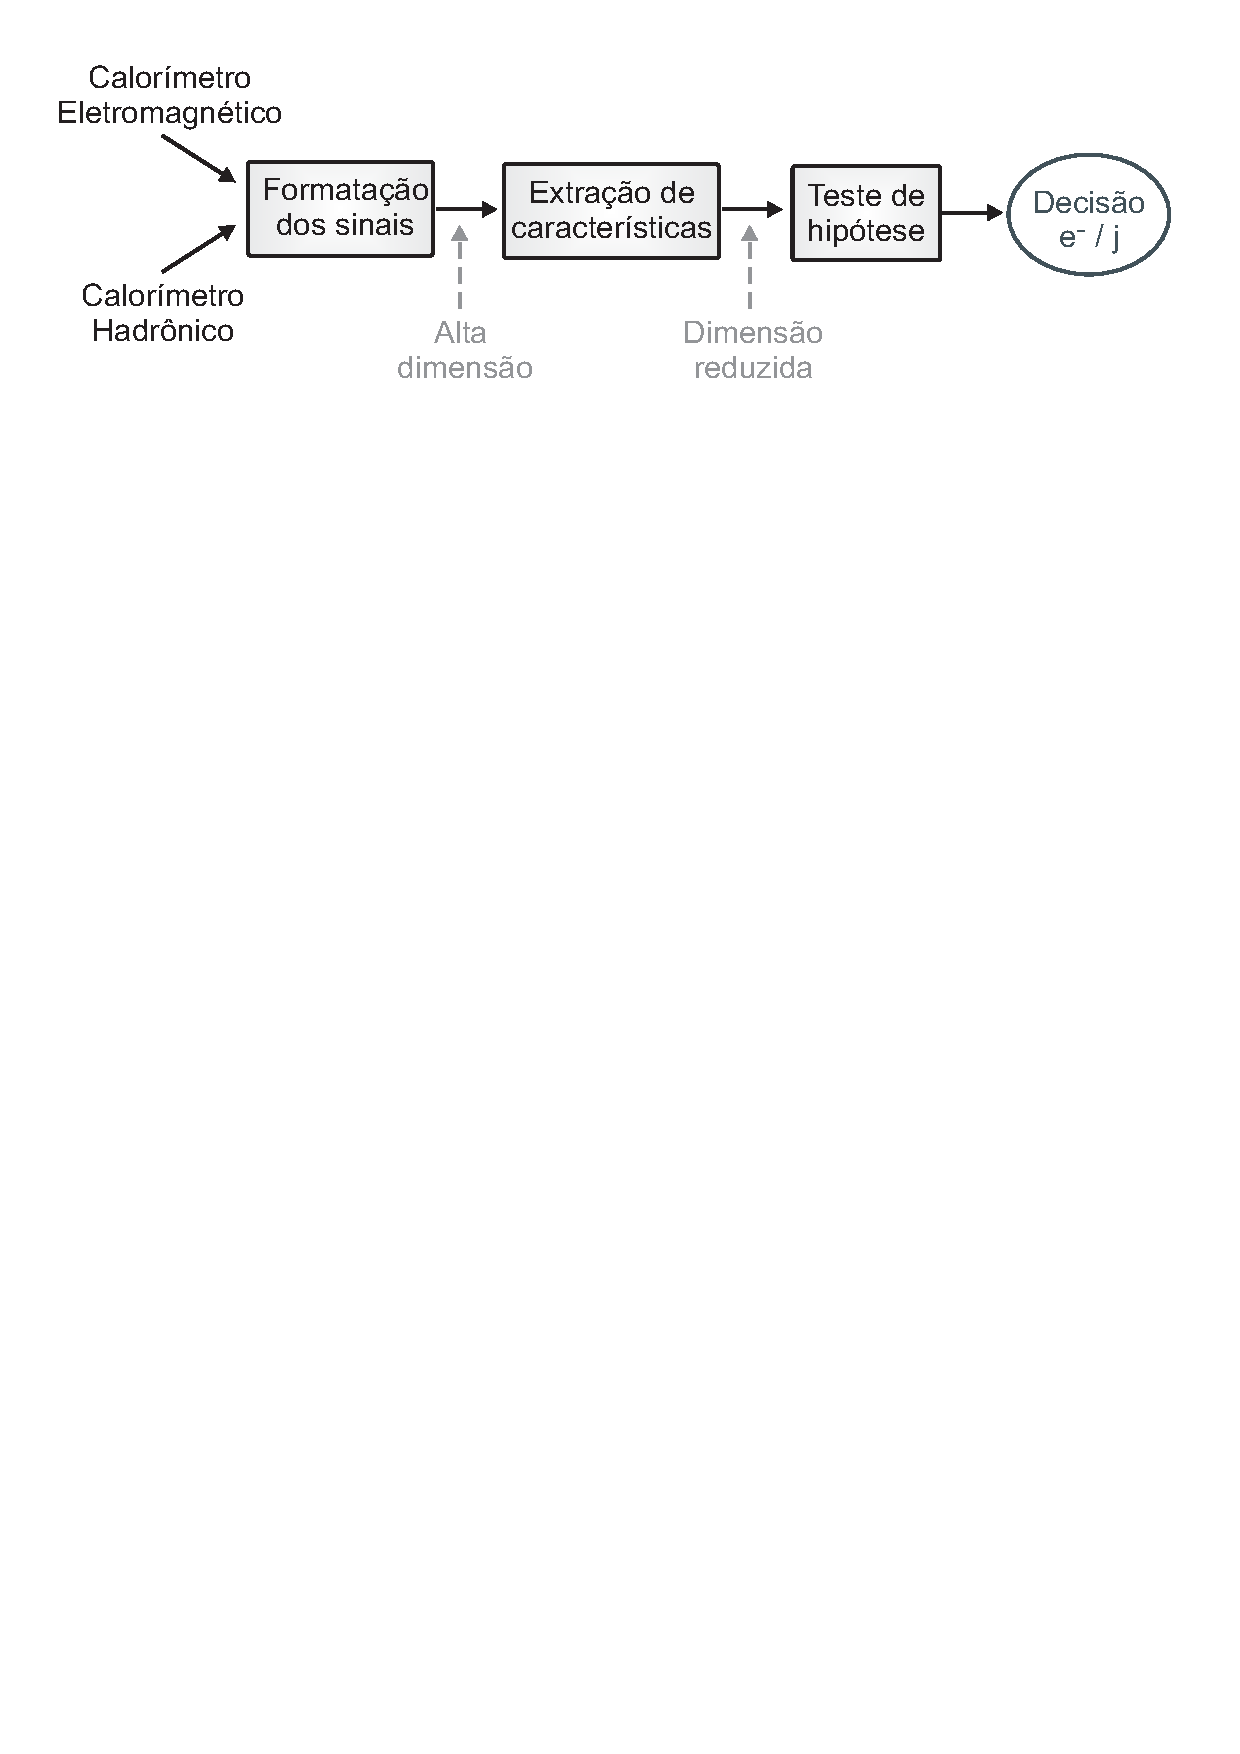
\includegraphics[width=7cm]{teste}
\caption{Diagrama do Modelo Padr�o mostrando as part�culas
elementares incluindo o, ainda n�o confirmado, boson de Higgs,
extra�do de \cite{livro:fisica1:2006}.} \label{SM}
\end{figure}

    \chapter{Introdu��o}

O processamento estat�stico de sinais encontra aplica��es nas
diversas �reas do conhecimento, desde medicina e sa�de p�blica at�
as bolsas de valores. Seu uso pode simplificar as tarefas de
an�lise de dados e classifica��o, pois permite mapear o conjunto de sinais em
um espa�o onde sua estrutura fundamental est� mais acess�vel.

Este trabalho descreve a aplica��o das t�cnicas de processamento
estat�stico no sistema de filtragem (detec��o) \textit{online} de 
um detector de part�culas elementares de altas energias. O objetivo � 
extrair caracter�sticas relevantes para guiar o
processo de identifica��o das part�culas.


\section{Contexto}

Com os constantes avan�os tecnol�gicos dos sistemas eletr�nicos de
aquisi��o de informa��es, � crescente a necessidade de t�cnicas
eficientes para o processamento \textit{online} de sinais. As
grandezas f�sicas s�o registradas por elementos sensores, que podem
ser �nicos (como na medi��o da velocidade de um motor), ou
combinados aos milhares para obter o resultado final (como na
captura de v�deo e imagem digitais).

Em aplica��es onde a fina granularidade da informa��o � necess�ria
para des\-cre\-ver adequadamente o processo f�sico em quest�o, e
sinais com alta dimens�o s�o assim gerados por sistemas de medi��o
compostos por um n�mero elevado de sensores, o custo computacional
geralmente � alto. Em alguns casos, a informa��o dispon�vel pode
estar segmentada, pois foi produzida a partir de conjuntos de
sensores com caracter�sticas distintas.

Se h� a necessidade de uma resposta r�pida, pode ser utilizada a
combina��o de t�cnicas de compacta��o de sinais e processamento
distribu�do. O cen�rio pode ficar ainda mais complicado quando o volume
de dados � alto e o problema a ser resolvido apresenta elevado grau
de complexidade.

O ambiente de aplica��o deste trabalho � o sistema \textit{online}
de filtragem do ATLAS (\textit{A Toroidal LHC
Aparatus})~\cite{article:ATLAS:2008}, maior detector de prop�sito
geral do acelerador de part�culas LHC (\textit{Large Hadron
Collider})~\cite{article:LHC:2008}. O LHC entrou em opera��o no
final de 2008, logo depois, passou por reparos no sistema de
resfriamento de um dos seus supercondutores, voltando a operar no
final de 2009.

No LHC, os sinais de interesse s�o raros, est�o imersos em um
intenso ru�do de fundo e a perda de um desses eventos compromete
severamente o desempenho dos detectores. Neste caso, � necess�ria
uma estrat�gia de filtragem capaz de remover, ou pelo menos atenuar
a intensidade do ru�do sem perder os eventos de interesse.

Combinado a isso, a taxa de ocorr�ncia de eventos � extremamente
elevada, fazendo com que o intervalo entre eventos consecutivos seja
extremamente pequeno. Considerando ainda que os detectores s�o
altamente segmentados e apresentam fina granularidade de c�lulas
detectoras, a quantidade de informa��o produzida � enorme. Neste
contexto, a sele��o de eventos precisa ser realizada de modo
\textit{online} e sob severas restri��es no tempo de processamento.

T�cnicas que utilizam informa��es da estat�stica dos sinais, como
An�lise de Componentes Principais (PCA - \textit{Principal Component
Analysis})~\cite{book:pca:2002}, An�lise de Componentes
Independentes ICA (\textit{Independent Component Analysis})
\cite{book:oja:2001} e Redes Neurais Artificiais (RNA)
\cite{haykin:nn:2008}, s�o frequentemente utilizadas na solu��o de
problemas onde h� a necessidade de processamento veloz, flex�vel e
eficiente.
%
%A An�lise de Componentes Principais � uma t�cnica que utiliza
%informa��es da estat�stica de segunda ordem para obter uma
%transforma��o onde os sinais na nova base s�o ortogonais e est�o nas
%dire��es de m�xima vari�ncia do processo. Eliminando-se as
%componentes de menor energia (vari�ncia) pode-se compactar o sinal
%mantendo a maior parte da informa��o necess�ria para sua
%reconstru��o.
%
%A An�lise de Componentes Independentes  busca extrair
%caracter�sticas ocultas em um conjunto de sinais, utilizando para
%isso informa��es da estat�stica de ordem superior. As
%caracter�sticas encontradas podem ser utilizadas para discrimina��o
%de classes de sinais diferentes ou para facilitar a an�lise da
%informa��o.

%As Redes Neurais Artificiais \cite{haykin:nn:2008} t�m um campo de
%aplica��o bastante amplo em processamento de sinais. Podem ser
%utilizadas, por exemplo, em reconhecimento de padr�es, classifica��o
%e filtragem n�o linear. As informa��es da estat�stica de ordem
%superior s�o utilizadas implicitamente atrav�s do uso de fun��es de
%ativa��o n�o lineares. As RNA podem utilizar treinamento
%supervisionado ou n�o-supervisionado.

\section{Motiva��o}

Desde o final do s�culo 19, quando foi descoberto o el�tron, o
estudo da f�sica de part�culas elementares de altas energias, ou simplesmente f�sica
de altas energias (HEP \textit{High-Energy Physics}), teve um crescimento acentuado. Na d�cada de 1950, com
o uso dos aceleradores, foram descobertas centenas de novas
part�culas. A f�sica de part�culas de altas energias pretende
encontrar os componentes fundamentais da mat�ria e descrever suas
formas de intera��o.

O LHC \cite{article:LHC:2008} � o maior e mais potente acelerador de part�culas da atualidade e est� em opera��o 
no CERN (Organiza��o Europ�ia para Pesquisa
Nuclear) desde 2008. Ao operar na m�xima capacidade, produzir� uma taxa de colis�es que
chegar� a 40MHz. Entretanto, as assinaturas de interesse ocorrer�o
numa freq��ncia muito menor, o que faz do sistema de filtragem
\textit{online} um componente fundamental para os detectores.

O ATLAS \cite{article:ATLAS:2008} � um detector de prop�sito geral do LHC e est� posicionado em um dos pontos de 
colis�o. Entre os principais objetivos do ATLAS, pode-se destacar a
busca pela part�cula conhecida como \textit{b�son de Higgs}, que
segundo estudos te�ricos seria respons�vel por interagir com as
part�culas fornecendo-lhes massa \cite{livro:fisica1:2006}. A
part�cula de Higgs ainda n�o foi verificada experimentalmente.

Parcela importante das informa��es necess�rias para a caracteriza��o
dos eventos � obtida do sistema de calor�metros, que, no ATLAS, � subdividido
em 7 camadas. Os calor�metros s�o medidores de energia compostos por um grande n�mero de
sensores (c�lulas). Ao interagirem com o material do calor�metro as part�culas perdem energia 
(e consequentemente velocidade). As c�lulas dos calor�metros quantificam a
energia perdida pelas part�culas incidentes e a informa��o do perfil de deposi��o de energia � utilizada 
para a caracteriza��o do tipo de part�cula.

%Algumas delas s�o inst�veis e apenas existem por um curto per�odo de
%tempo, sendo rapidamente transformadas em outras menos energ�ticas.

%Operando em m�xima capacidade o LHC ir� colidir feixes de pr�tons a
%cada 25 ns. Numa colis�o uma quantidade enorme de energia ser�
%transformada em um grande n�mero de part�culas. A maior parte da
%informa��o a ser gerada j� foi visualizada em experimentos
%anteriores, n�o sendo relevante para os detectores do LHC. A chamada
%nova f�sica, ou f�sica de interesse, representa uma pequena parcela
%das informa��es produzidas. Os eventos da f�sica de interesse devem
%ser armazenados para futura an�lise detalhada. Percebe-se, ent�o, a
%import�ncia do sistema \textit{online} de filtragem e classifica��o,
%que deve ser capaz de identificar os eventos de interesse dentro do
%intenso ru�do de fundo. Uma eficiente filtragem \textit{online}
%permite o processo de busca e an�lise \textit{offline}.

Os objetivos principais dos sistemas de filtragem \textit{online} em
experimentos de f�sicas de altas energias s�o maximizar a
probabilidade de detec��o (e consequente armazenamento) dos eventos
de interesse, e minimizar a probabilidade de armazenar eventos n�o
desejados (ru�do de fundo ou falso-alarme). Em um ambiente como este, a alta
dimens�o dos dados, o intenso ru�do de fundo e o curto tempo de
resposta exigido s�o s�rios
entraves para o processamento e classifica��o \textit{online} de
eventos.

No ATLAS, o sistema \textit{online} de filtragem (\textit{trigger})
de eventos � composto por tr�s n�veis de sele��o sequenciais. O ru�do de fundo � gradualmente 
reduzido a cada n�vel de filtragem, esperando-se armazenar, em
m�dia permanente, uma taxa m�xima de 200 Hz \cite{LI:ATLAS:1992}. 
Considerando que a freq��ncia de colis�es � 40 MHz, deve haver uma
redu��o de $2\times 10^5$ vezes.

%O primeiro n�vel (L1 -
%\textit{Level-One}), por restri��es de tempo de resposta e
%quantidade de informa��o a ser processada, foi implementado em
%\textit{hardware} dedicado, objetivando reduzir a taxa de eventos
%para 10kHz. Este n�vel opera com lat�ncia menor que $2,5\mu s$. O
%segundo n�vel (L2 - \textit{Level-Two}) e o filtro de eventos (EF -
%\textit{Event Filter}) correspondem � filtragem de alto n�vel (HLT -
%\textit{high level trigger}) e, em conjunto, precisam reduzir de
%10kHz para 200Hz a freq��ncia dos eventos. Devido � lat�ncia um
%pouco maior, da ordem de $10ms$ para o segundo n�vel e alguns
%segundos para o filtro de eventos, essas etapas ser�o realizadas em
%\textit{software} atrav�s de um sistema de processamento
%distribu�do, que utiliza centenas de processadores semelhantes aos
%de computadores pessoais (PC). Algoritmos desenvolvidos pela
%colabora��o do ATLAS est�o prontos para operar nos diversos canais e
%n�veis de filtragem existentes.

No contexto dos diversos canais de interesse para a f�sica no ATLAS,
este trabalho se encontra focado na discrimina��o el�tron/jato
(e$^-/$j). Os el�trons podem estar envolvidos em fen�menos como o decaimento 
do b�son de Higgs, supersimetria e a descoberta de novos b�sons. Por�m, em
termos de calorimetria, alguns jatos podem apresentar um perfil de
deposi��o de energia semelhante ao dos el�trons. Portanto, os jatos
representam ru�do de fundo no processo de identifica��o de el�trons.
Apenas uma parcela dos candidatos a el�trons aceitos pelo
primeiro n�vel s�o realmente el�trons; cabendo � filtragem de alto
n�vel reduzir ainda mais o ru�do de fundo, mantendo a maior parte das assinaturas de
interesse.

Considerando a alta taxa de eventos e a intensidade do ru�do de
fundo produzidos pelo LHC, a busca por algoritmos de filtragem
\textit{online} mais eficientes � uma tarefa importante.
A redu��o no n�mero de eventos n�o relevantes (ru�do de fundo)
armazenados em m�dia permanente significa maior efici�ncia na
an�lise \textit{offline} dos eventos de interesse e redu��o do
espa�o (m�dia) necess�rio para armazenamento.

Neste trabalho est�o sendo propostas alternativas para o algoritmo
padr�o de detec��o de el�trons em uso atualmente no segundo
n�vel de filtragem (L2) do detector ATLAS. Os algoritmos desenvolvidos
apresentam maior efici�ncia de discrimina��o e tempo de
processamento dentro das restri��es do L2.

\section{Trabalhos Anteriores}

Considerando os desafios existentes no ambiente de filtragem
\textit{online} do \linebreak ATLAS, no qual os sinais s�o adquiridos
com fina segmenta��o, est�o imersos em intenso ru�do de fundo e as
assinaturas de interesse s�o raras, t�cnicas avan�adas de extra��o
de caracter�sticas podem ser utilizadas para melhorar a efici�ncia
de classifica��o.

No trabalho~\cite{article:seixas:1996} foi inicialmente proposto o uso de um classificador neural 
supervisionado (arquitetura \textit{Perceptron} de M�ltiplas Camadas) para o canal
el�tron/jato do segundo n�vel de filtragem do detector ATLAS. Utilizando informa��o especialista a respeito 
do problema, os sinais medidos nos calor�metros s�o formatados em an�is conc�ntricos de deposi��o de energia.
A formata��o dos an�is preserva a informa��o discriminante do perfil de deposi��o
de energia e compacta a informa��o (de ~1000 c�lulas para 100 an�is).

Em \cite{tese:andre:2006} o sistema neural de identifica��o de el�trons (que ficou conhecido como \textit{Neural Ringer}) 
foi implementado no sistema (\textit{software}) de filtragem do ATLAS.
Numa compara��o de desempenho entre o Neural Ringer e o discriminador oficial do ATLAS 
(T2Calo) foi mostrado que o \textit{Ringer} apresenta desempenho superior e � capaz de
operar dentro da janela de tempo permitida para o L2. 

No trabalho \cite{tese:torres:2010} alguns m�todos de compacta��o como An�lise de Componentes
Principais (PCA - \textit{Principal Component Analysis}) \cite{book:pca:2002} e Componentes Principais 
de Discrimina��o (PCD - \textit{Principal Componentes of Discrimination}) \cite{seixas:pcd:1995} foram 
aplicados, em conjunto com o modelo linear da An�lise de Componentes Independentes 
(ICA - \textit{Independent Component Analysis}) \cite{book:oja:2001}, sobre os sinais em an�is como 
um pr�-processamento para o classificador neural. A utiliza��o destas t�cnicas de
extra��o de caracter�sticas e compacta��o permitiu aumento do desempenho de classifica��o e redu��o do tempo
necess�rio para tomada de decis�o. Neste trabalho foi realizada tamb�m uma implementa��o otimizada 
do \textit{Neural Ringer} no sistema \textit{online} de filtragem do ATLAS operando como uma sub-rotina do T2Calo. 
Neste nova vers�o o custo computacional foi reduzido e o Ringer utiliza uma parte do processamento realizado pelo 
T2Calo.

\section{Objetivos}

Os calor�metros s�o projetados para serem detectores lineares, por�m, diversas fontes de n�o-linearidades
podem surgir numa implementa��o pr�tica \cite{book:wigmans:2000}. Neste caso, um m�todo n�o-linear de extra��o
de caracter�sticas talvez seja mais indicado para o problema.

O principal objetivo do presente trabalho � avaliar o desempenho obtido pelo discriminador \textit{Neural Ringer}
quando os sinais em an�is s�o pr�-processados por m�todos de extra��o de caracter�sticas baseados
no modelo n�o-linear da an�lise de componentes independentes (NLICA - \textit{Nonlinear Independent 
Component Analysis})~\cite{book:almeida:2006}. 

Neste contexto, foram utilizados diversos modelos e algoritmos de estima��o da NLICA e seus resultados 
comparados em termos da efici�ncia de discrimina��o e do tempo de processamento. Foi proposta tamb�m a 
segmenta��o dos processos de extra��o de caracter�sticas e classifica��o, visando explorar adequadamente 
toda segmenta��o e granularidade dispon�veis no detector.

O modelo da NLICA foi originalmente definido para realizar a extra��o de caracter�sticas de modo n�o-supervisionado. 
Ou seja, n�o h� como garantir que a transforma��o seja �til para o problema de classifica��o (no sentido 
de revelar caracter�sticas discriminantes). Neste trabalho foram propostas modifica��es no modelo tradicional 
da NLICA visando a estima��o de componentes com maior poder de discrimina��o entre as classes.

\section{Metodologia}

O projeto dos discriminadores de part�culas foi realizado
a partir de um conjunto de eventos simulados. Estas simula��es, por t�cnicas de Monte Carlo~\cite{book:montecarlo:2004},
consideram todas as caracter�sticas f�sicas do detector e do
acelerador. Foram utilizados, tamb�m, conjuntos de dados experimentais obtidos na
fase inicial de opera��o do LHC. Sabe-se que
os raios c�smicos representam ru�do de fundo para o canal el�tron/jato, pois produzem m�ons no detector.
Assim, os algoritmos propostos foram tamb�m testados para uma base de dados
composta de eventos de raios c�smicos, visando verificar a capacidade de rejei��o para esse sinal. Uma outra an�lise utilizou eventos de colis�o obtidos recentemente na fase inicial de opera��o do LHC.

Foram aplicados diversos algoritmos para estimar o modelo n�o-linear das componentes independentes (NLICA).
Visando explorar adequadamente as caracter�sticas do detector, o modo de executar as tarefas de extra��o de caracter�sticas e classifica��o foi variado entre as abordagens segmentada (onde o processamento � feito a n�vel de cada camada do calor�metro) e n�o-segmentada (quando os sinais em an�is, gerados a partir de todas as camadas, s�o concatenados em um �nico vetor).

Entre os diversos modelos existentes para a a estima��o da NLICA, neste trabalho foram utilizados os modelos sem restri��o estrutural (atrav�s dos mapas auto-organiz�veis) e o modelo p�s n�o-linear (que restrige os mapeamentos n�o-lineares poss�veis a uma mistura linear seguida de fun��es n�o-lineares aplicadas a cada componente desta mistura). A ICA Local, que � um modelo diretamente ligado ao da NLICA tamb�m foi utilizada. Para cada modelo proposto foi realizado um estudo comparativo de desempenho com o Neural Ringer quando este opera diretamente sobre os sinais em an�is. 

Considerando o sistema de classifica��o neural, foi proposta a utiliza��o de classificadores especilistas na informa��o de cada camada do calor�metro. Diversos modos de combinar a informa��o deste conjunto de classificadores foram testados. Deste modo verificou-se que h� redund�ncia de informa��o entre as diversas camadas do calor�metro. Pode-se, ent�o, obter o mesmo desempenho de discrimina��o utilizando-se apenas uma parcela das informa��es dispon�veis e, assim, contribuir para a redu��o do tempo de processamento.

\section{Conte�do do trabalho}

No Cap�tulo 2 ser� apresentado o ambiente cient�fico no qual o
trabalho est� sendo desenvolvido, contextualizando o detector de
part�culas ATLAS, o acelerador LHC e o CERN. Uma descri��o dos sistemas 
de \textit{trigger online} em experimentos de f�sica de altas
energias e ,mais especificamente, no detector ATLAS ser�o apresentadas 
no Cap�tulo 3.

� descrito, no Cap�tulo 4, o processo de sele��o de el�trons utilizando informa��es de calorimetria no 
detector ATLAS. No Cap�tulo 5, ser�o mostrados os fundamentos te�ricos das t�cnicas
de extra��o de caracter�sticas e teste de hip�tese que ser�o
utilizadas para a otimiza��o do sistema de filtragem do ATLAS.

A metodologia empregada no desenvolvimento deste trabalho � descrita no Cap�tulo 6. Os conjuntos de dados utilizados
para desenvolvimento e teste dos sistemas de classifica��o propostos ser�o apresentados no Cap�tulo 7.

Os resultados obtidos ser�o apresentadas no Cap�tulo~8. As
conclus�es e os futuros trabalhos s�o os t�picos abordados no
Cap�tulo~9.

Nos Ap�ndices A e B s�o fornecidas as bases matem�ticas para uma
melhor compreens�o, respectivamente, dos algoritmos de extra��o de caracter�sticas e classifica��o utilizados. 
Finalmente, no Ap�ndice C ser�o listadas
as publica��es produzidas com os resultados obtidos neste trabalho.

    %comecei a trabalhar na versao final em 15 de junho de 2009

\chapter{F�sica de Part�culas e o detector ATLAS}
\label{cap_atlas}

Os experimentos de F�sica de Part�culas Elementares t�m como
principais objetivos a confirma��o de modelos desenvolvidos
teoricamente e a identifica��o de novos fen�menos. O experimento
LHC~\cite{article:LHC:2008} � o maior acelerador de part�culas j�
desenvolvido e quando operando em m�xima capacidade, ser�o gerados
aproximadamente $10^9$ intera��es por segundo. Os detectores s�o
respons�veis por selecionar, dentro de um conjunto enorme, os
eventos de real interesse, que s�o bastante raros. O projeto e a
montagem do detector ATLAS (\textit{A Thoroidal LHC Apparatus})
\cite{article:ATLAS:2008} foram conduzidos por uma cola\-bo\-ra��o
de 36 pa�ses, conhecida como \textit{ATLAS Collaboration}, contando
com pesquisadores de mais de 150 universidades e centros de
pesquisa~\cite{Homepage:ATLAS}. Sendo um dos detectores de prop�sito
geral do experimento LHC, o ATLAS tem formato cil�ndrico e foi
projetado para cobrir um �ngulo s�lido pr�ximo a $4\pi$ ao redor da
regi�o de colis�o.


\section{Panorama geral da f�sica de part�culas elementares}

A no��o de que a mat�ria � composta por um conjunto de constituintes
elementares existe h� mais de 2000 anos, desde o tempo dos fil�sofos
gregos~\cite{book:fernow:1986}. No decorrer do s�culo 20, a
compreens�o dos componentes elementares da mat�ria forneceu �
comunidade cient�fica mundial informa��es importantes a res\-peito
das leis fundamentais da natureza. O estudo da f�sica de part�culas
elementares teve in�cio no final do s�culo 19, quando foi descoberto
o el�tron, experimentando um crescimento acen\-tua\-do na d�cada de
1950, quando foram descobertas centenas de novas part�culas. A
partir de sua cria��o em 1954, o CERN (Centro Europeu para Pesquisa
Nuclear) contribuiu significativamente nesse processo.

Inicialmente, pensava-se que a mat�ria era constitu�da de part�culas
subat�\-micas, chamadas el�trons, pr�tons e n�utrons. Mais tarde,
descobriu-se que os pr�tons e n�utrons s�o compostos de quarks. Hoje
sabe-se que toda a mat�ria no universo � composta de l�ptons e
quarks. Existem ainda outras part�culas elementares que s�o
respons�veis por promover a intera��o entre l�ptons e quarks.
Juntamente com as descobertas experimentais, estudos te�ricos
possibilitaram o desenvolvimento do Modelo Padr�o
(SM-\textit{Standard Model})~\cite{livro:fisica1:2006} que descreve
e prev�, de forma unificada, o comportamento das part�culas e das
for�as de intera��o.

As caracter�sticas e propriedades dos processos nucleares dependem
da ener\-gia envolvida. A unidade de energia mais utilizada, neste
contexto, � o el�tron-volt (eV) e seus m�ltiplos (MeV, GeV ou TeV).
O el�tron-volt � definido como a energia necess�ria para aumentar o
potencial el�trico de um el�tron em 1 volt (em unidades do Sistema
Internacional - SI temos: 1eV$=$1,6$\times
10^{-19}$J)~\cite{book:martin:2006}. Os fen�menos produzidos quando
a energia das part�culas � menor que $20MeV$ s�o chamados de f�sica
a baixas energias. A faixa entre $20MeV$ e $400MeV$ corresponde �
f�sica a energias intermedi�rias, e finalmente, fen�menos com
energia superior a $400MeV$ s�o estudados na f�sica a altas
energias~\cite{book:chung:2001}.

%, extra�do de \cite{livro:fisica1:2006}

Os experimentos realizados a partir do in�cio da d�cada de 1970
foram fundamentais para o desenvolvimento e teste do Modelo Padr�o,
mas tamb�m despertaram d�vidas a respeito de quest�es que n�o s�o
completamente respondidas. O SM (ver Figura \ref{SM}), divide as
part�culas elementares em quarks e l�ptons. Existem seis tipos de
l�
ptons (el�tron, m�on, tau e tr�s neutrino) e seis tipos de quarks
(\textit{up}, \textit{down}, \textit{charm}, \textit{strange},
\textit{top} e \textit{bottom}).

\begin{figure}[h!] \centering
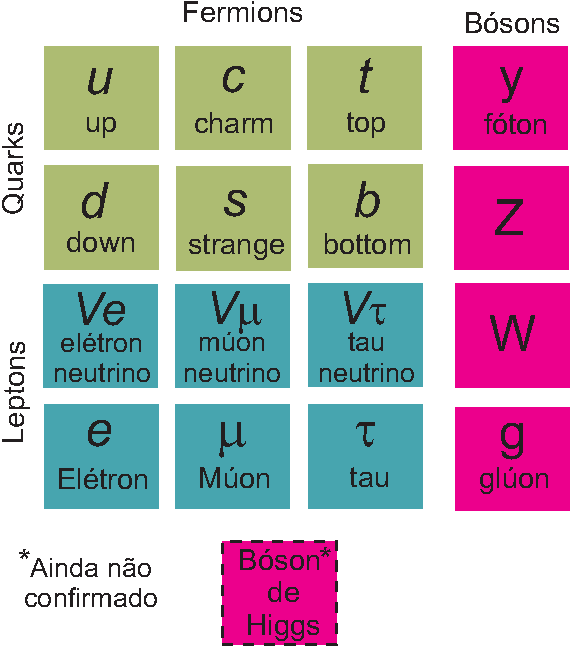
\includegraphics[width=7cm]{cap2_sm}
\caption{Diagrama do Modelo Padr�o, mostrando as part�culas
elementares incluindo o, ainda n�o confirmado, b�son de Higgs.}
\label{SM}
\end{figure}

Atualmente s�o conhecidas quatro formas de intera��o (ou
acoplamento) entre as part�culas elementares, s�o elas
eletromagn�tica, gravitacional, fraca e forte. A for�a gravitacional
� predominante entre corpos massivos separados por longas
dist�ncias. Entre part�culas, onde a massa � da ordem de
$10^{-27}$Kg, a intera��o gravitacional tem intensidade muito baixa.
Para dist�ncias maiores que $10^{-13}$cm, a for�a eletromagn�tica
domina, enquanto que para distancias menores, as intera��es forte e
fraca se destacam. A intensidade relativa (em compara��o com a
intera��o forte) dos quatro tipos de intera��o � mostrada na Tabela
\ref{tab_forcas} \cite{book:mist:2003}.

\begin{table}[b!]
\centering
\caption{Intensidade relativa (em compara��o com a intera��o forte)
dos diversos tipos de intera��o.}\vspace{.3cm}
\begin{tabular}{cc }
  \hline
  % after \\: \hline or \cline{col1-col2} \cline{col3-col4} ...
  \textbf{Intera��o} & \textbf{Intensidade Relativa} \\  \hline
  Forte  &  1 \\
  Eletromagn�tica  & $10^{-2}$\\
  Fraca & $10^{-5}$ \\
  Gravitacional & $10^{-39}$ \\
  \hline
\end{tabular}
\label{tab_forcas}
\end{table}

Existem algumas teorias que descrevem como as intera��es elementares
ocorrem. A eletrodin�mica qu�ntica (QED - \textit{Quantum
Eletrodynamics}) considera que os processos el�tricos e magn�ticos
acontecem a partir da intera��o fundamental entre dois el�trons, com
a troca de um f�ton. O f�ton � a part�cula mediadora da intera��o
eletromagn�tica.

De modo semelhantes s�o definidos os outros tipos de intera��o. Para
a intera��o forte, as part�culas mediadoras s�o os gl�ons. Os b�sons
W e Z mediam a intera��o fraca e o gr�viton a intera��o
gravitacional. A teoria da cromodin�mica qu�ntica (QCD -
\textit{Quantum Chromodynamics}) \cite{book:QCD:2003}, por exemplo,
descreve como os quarks e gl�ons interagem para formar os hadrons
(pr�tons e neutrons s�o exem\-plos de h�drons). Uma diferen�a entre
a QED e a QCD � que na �ltima, os quarks e gl�ons n�o s�o observados
como part�culas livres (mas apenas na forma de h�drons), em oposi��o
aos el�trons e f�tons da QED. Mesmo em colis�es de alta energia,
quando quarks s�o produzidos, eles se afastam rapidamente uns dos
outros, e antes que possam ser observados, se convertem em ``jatos"
de h�drons (ou jatos hadr�nicos)~\cite{book:martin:2006}.

Considerando uma teoria atualmente aceita pela f�sica te�rica
(conhecida como \textit{Gauge Invariance}) e as part�culas e formas
de intera��o j� verificadas experimentalmente, todas as part�culas
elementares teriam massa nula. Esta previs�o � contr�ria aos
resultados experimentais e somente pode ser corrigida assumindo-se
que existe um outro tipo de intera��o. Esta intera��o foi prevista
pelo cientista ingl�s Peter Higgs em 1964, tendo como part�cula
mediadora o b�son de Higgs, que � respons�vel por fornecer massa �s
part�culas~\cite{book:martin:2006}. A exist�ncia do b�son de Higgs �
a mais importante previs�o do modelo padr�o ainda n�o verificada
experimentalmente e sua busca � de m�xima import�ncia para a f�sica
de part�culas.

Nas �ltimas d�cadas, os experimentos com aceleradores de part�culas
se tornaram gigantescos empreendimentos envolvendo milhares de
f�sicos e engenheiros com contribui��o financeira e intelectual de
dezenas de pa�ses. Os aceleradores usam for�a eletromagn�tica para
aumentar a energia de part�culas est�veis e carregadas
eletricamente. As part�culas s�o injetadas na m�quina por
dispositivos que produzem uma fonte de part�culas de alta
intensidade e baixa energia. Quanto �s caracter�sticas construtivas,
os aceleradores podem ser divididos em alvo-fixo ou colisionadores
de feixes. Nos aceleradores de alvo-fixo, as part�culas s�o
aceleradas at� a m�xima energia, quando o feixe � retirado da
m�quina e direcionado a um alvo estacion�rio. Nos colisionadores,
feixes de part�culas s�o acelerados e quando a energia desejada �
atingida, os feixes s�o colocados em rota de colis�o em alguns
pontos espec�ficos do percurso. Quanto ao percurso dos feixes, os
aceleradores podem ser lineares ou circulares
\cite{book:martin:2006}.

Imediatamente ap�s a colis�o, uma grande quantidade de part�culas
elementares � produzida. Algumas delas s�o est�veis, por�m outras
t�m curt�ssimo tempo de vida. Os el�trons e pr�tons, por exemplo,
t�m vida m�dia superior a $10^{23}$ anos, enquanto os m�ons podem
ter vida m�dia da ordem de $10^{-6}$ segundos
\cite{book:chung:2001}. Para que todos os eventos sejam corretamente
identificados, um complexo sistema de detec��o precisa ser
constru�do.

A massa (m) das part�culas � usualmente expressa em fun��o da
energia equi\-va\-lente ($m=E/c^2$, onde $c$ � a velocidade da luz e
$E$ a energia). Os b�sons W e Z, por exemplo, t�m massa de 80 e 91
GeV/c$^2$ (onde 1GeV/c$^2$=1,78$\times 10^{-27}$ kg). Na Tabela
\ref{tab_massa}, s�o mostradas as massas de algumas part�culas
importantes. Ainda n�o � poss�vel determinar a massa esperada para o
b�son de Higgs, por�m, considerando o conhe\-ci\-men\-to adquirido
com os experimentos operados antes do LHC, sua massa deve ser maior
que 115 GeV/c$^2$ \cite{livro:fisica1:2006}.

O acelerador LHC (\textit{Large Hadron Collider} - Grande
Colisionador Hadr�nico)~\cite{article:LHC:2008,article:LHC:2002} em
opera��o no CERN (Centro Europeu para Pesquisa Nuclear)
\cite{Homepage:CERN}, ser� capaz de atingir energia de at� 14 TeV e
permitir � visualiza��o do b�son de Higgs, caso o Modelo Padr�o
esteja correto.

\begin{table}[h!]
\centering
\caption{Exemplos de valores da massa (em energia equivalente) de
algumas part�culas.}\vspace{.3cm}
\begin{tabular}{cc }
  \hline
  % after \\: \hline or \cline{col1-col2} \cline{col3-col4} ...
  \textbf{Part�cula} & \textbf{Massa (GeV/c$^2$)} \\  \hline
  El�tron  &  0,000511 \\
  Pr�ton  & 0,938 \\
  B�son W & 80 \\
  B�son Z & 91 \\
  B�son de Higgs ou outras novas part�culas & $>$115 \\
  \hline
\end{tabular}
\label{tab_massa}
\end{table}

Al�m da busca pelo b�son de Higgs, existem outras quest�es que
precisam ser respondidas em f�sica de part�culas. � um desejo antigo
dos f�sicos, desde Einstein, a unifica��o das teorias sobre as
for�as entre as part�culas, incluindo no Modelo Padr�o a for�a
gravitacional. O estudo da f�sica de part�culas tamb�m � fundamental
para o entendimento da natureza e origem do universo. Pretende-se,
por exemplo, descobrir informa��es sobre a composi��o da mat�ria
escura \cite{article:darkm:2005}, super-simetria
\cite{article:susy:1996} e viola��o de CP (do ingl�s \textit{Charge
Parity})~\cite{book:cpv:1999}.

Entre os laborat�rios que conduzem experimentos em f�sica de
part�culas os principais s�o: CERN, DESY \cite{Homepage:desy}, KEK
\cite{homepage:kek}, Fermilab \cite{Homepage:Fermilab}, SLAC
\cite{homepage:slac} e Brookhaven~\cite{Homepage:brookhaven},
localizados respectivamente na Su��a, Alemanha, Jap�o e os tr�s
�ltimos nos Estados Unidos.

O CERN, fundado em 1954, � atualmente um dos maiores centros de
pesquisas em f�sica de part�culas do mundo. Localizado em Genebra,
Su��a, funciona com base num complexo sistema de colabora��o
internacional, que envolve centenas de institui��es de pesquisa em
centenas de paises \cite{Homepage:CERN}.

\section{O acelerador LHC}

No CERN, foi projetado e constru�do o experimento LHC (\textit{Large
Hadron Collider}), que iniciou sua opera��o no final de 2008~\cite{article:LHC:2008,Homepage:lhc}. O LHC pode atingir n�veis de
energia de, aproximadamente, 14 TeV. O percurso do
acelerador, localizado na fronteira franco-su��a, � aproximadamente
circular, com 27 Km de comprimento, numa profundidade do solo que
varia de 50 a 150 metros (ver Figura \ref{mapaLHC}). Feixes de
pr�tons ser�o acelerados em sentidos opostos e direcionados para
colis�o nos centros dos detectores.

\begin{figure}[b!]
\centering
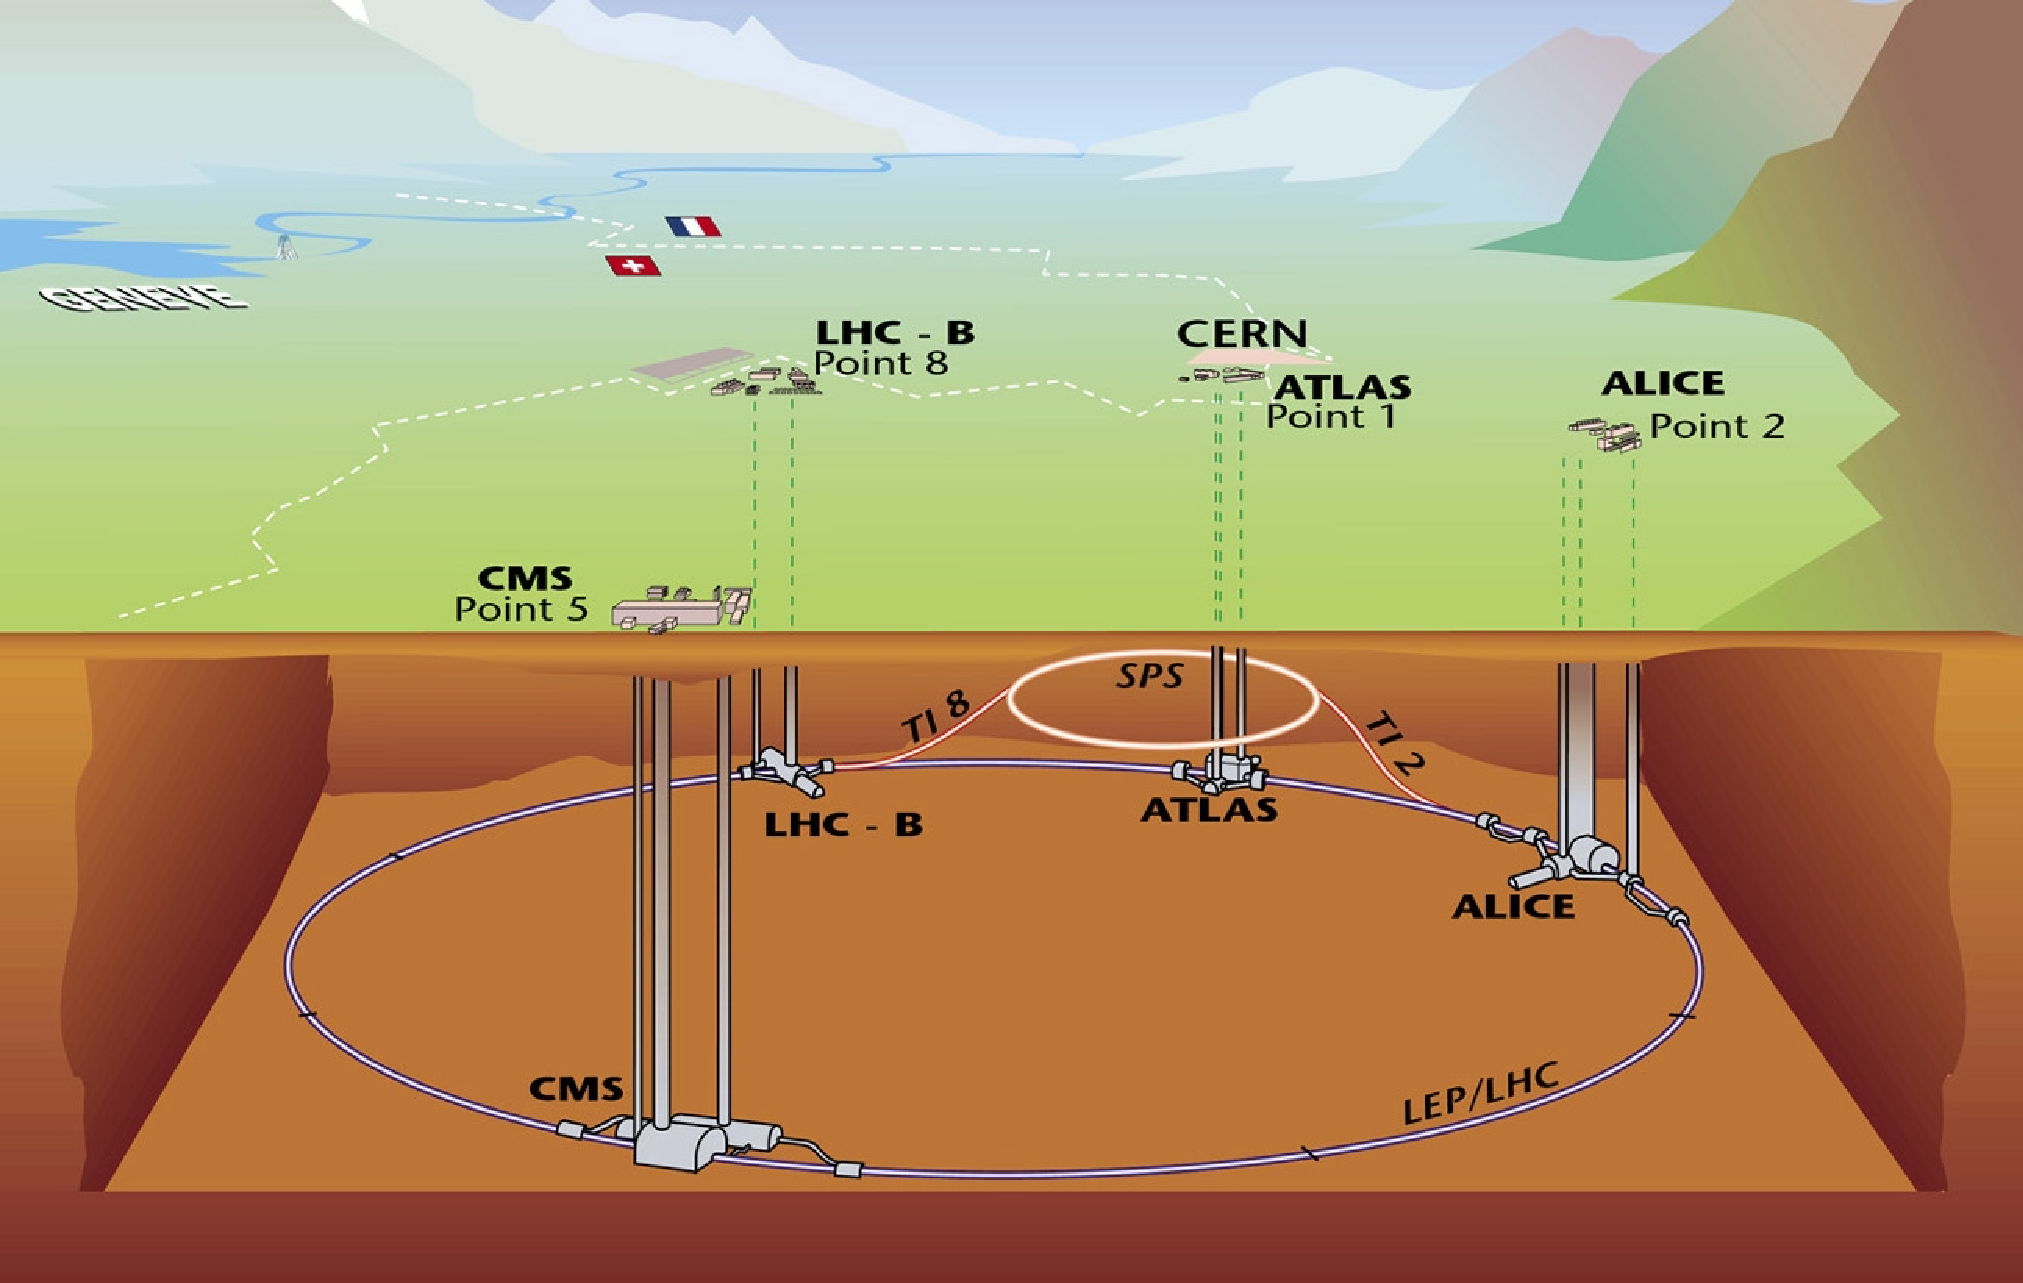
\includegraphics[width=15cm]{cap2_lhc_map2}
\caption{Mapa de localiza��o dos detectores do LHC.} \label{mapaLHC}
\end{figure}

O LHC tem 6 detectores com prop�sitos diferentes: ATLAS
\cite{article:ATLAS:2008}, CMS~\cite{article:CMS:2008},
LHCb~\cite{article:LHCb:2008}, LHCf~\cite{article:LHCf:2008}, ALICE
\cite{article:ALICE:2008} e TOTEM \cite{article:TOTEM:2008}. O ATLAS
e o LHCf est�o localizados em Meyrin, Su��a, o CMS e o TOTEM em
Cessy, Fran�a, o ALICE em St. Genis-Pouilly, Fran�a e o LHCb em
Ferney-Voltaire, Fran�a (os experimentos TOTEM e LHCf n�o s�o
mostrados na Figura \ref{mapaLHC} pois est�o em locais pr�ximos
respectivamente ao CMS e ATLAS). O ATLAS (\textit{A Toroidal LHC
AparattuS}) e o CMS (\textit{Compact Muon Solenoid}) s�o detectores
de prop�sito geral, enquanto os outros s�o dedicados a aplica��es
espec�ficas, como o LHCb, que � dedicado a explorar informa��es
sobre a f�sica proveniente dos h�drons do tipo \textbf{b} produzida
nas colis�es do LHC.

Quando operando em m�xima capacidade, o LHC ir� produzir colis�es de
feixes de pr�tons a cada 25 ns e atingir� energia 7 vezes maior que
o Tevatron, que � o acelerador de maior energia em opera��o
atual\-mente, funcionando no Fermilab.

O n�mero de colis�es por cent�metro quadrado produzidas por segundo
� chamado de luminosidade (L)~\cite{book:martin:2006}:
\begin{equation}\label{lumi}
    L=n\frac{N_1N_2}{A}f
\end{equation}
onde $n$ � o n�mero de feixes, $N_1$ e $N_2$ o n�mero de part�culas
em cada feixe, $A$ a �rea da se��o transversal do feixe e $f$ a
frequ�ncia de colis�o. Quanto maior a luminosidade do experimento,
maior a quantidade de informa��o (part�culas) gerada.

Quando operando numa luminosidade jamais alcan�ada
($10^{34}cm^{-2}s^{-1}$), o LHC deve atingir uma taxa de intera��es
da ordem de 1 GHz. No LHC, fatores como a alta taxa de intera��es,
as altas doses de radia��o, a multiplicidade de part�culas e largas
faixas de ener\-gia a cobrir, em conjunto com a necessidade de
medi��es precisas, definiram novos padr�es para o projeto dos
detectores.

A seguir, ser�o descritas, de modo geral, as principais
caracter�sticas do detector ATLAS.

\section{Caracter�sticas gerais do detector ATLAS}

Os m�todos de detec��o em f�sica t�m como princ�pio b�sico promover
intera��o entre as part�culas em estudo e um material conhecido,
produzindo informa��es sobre a natureza e as caracter�sticas da
pr�pria part�cula. Os instrumentos que possibilitam a medi��o
experimental destas quantidades f�sicas s�o chamados de detectores.
Em particular, os detectores de energia s�o chamados de
calor�metros. � medida que a energia envolvida aumenta, o sistema de
detec��o precisa ser mais sofisticado \cite{book:chung:2001}.

O ATLAS foi fruto do trabalho de uma grande colabora��o, que
envolveu milhares de f�sicos, engenheiros, t�cnicos e estudantes por
um per�odo de vinte anos de projeto, desenvolvimento, fabrica��o e
instala��o.

O detector ATLAS tem 45 m de comprimento, 25 m de altura e pesa
aproximadamente 7.000 toneladas, sendo dividido em subsistemas
dispostos em camadas. Conforme ilustrado na Figura \ref{atlas_diag},
os principais subsistemas s�o: detector de trajet�rias (ou de
tra�o), calor�metros eletromagn�tico e hadr�nico e os detectores de
m�ons.

\begin{figure}[h!]
\centering
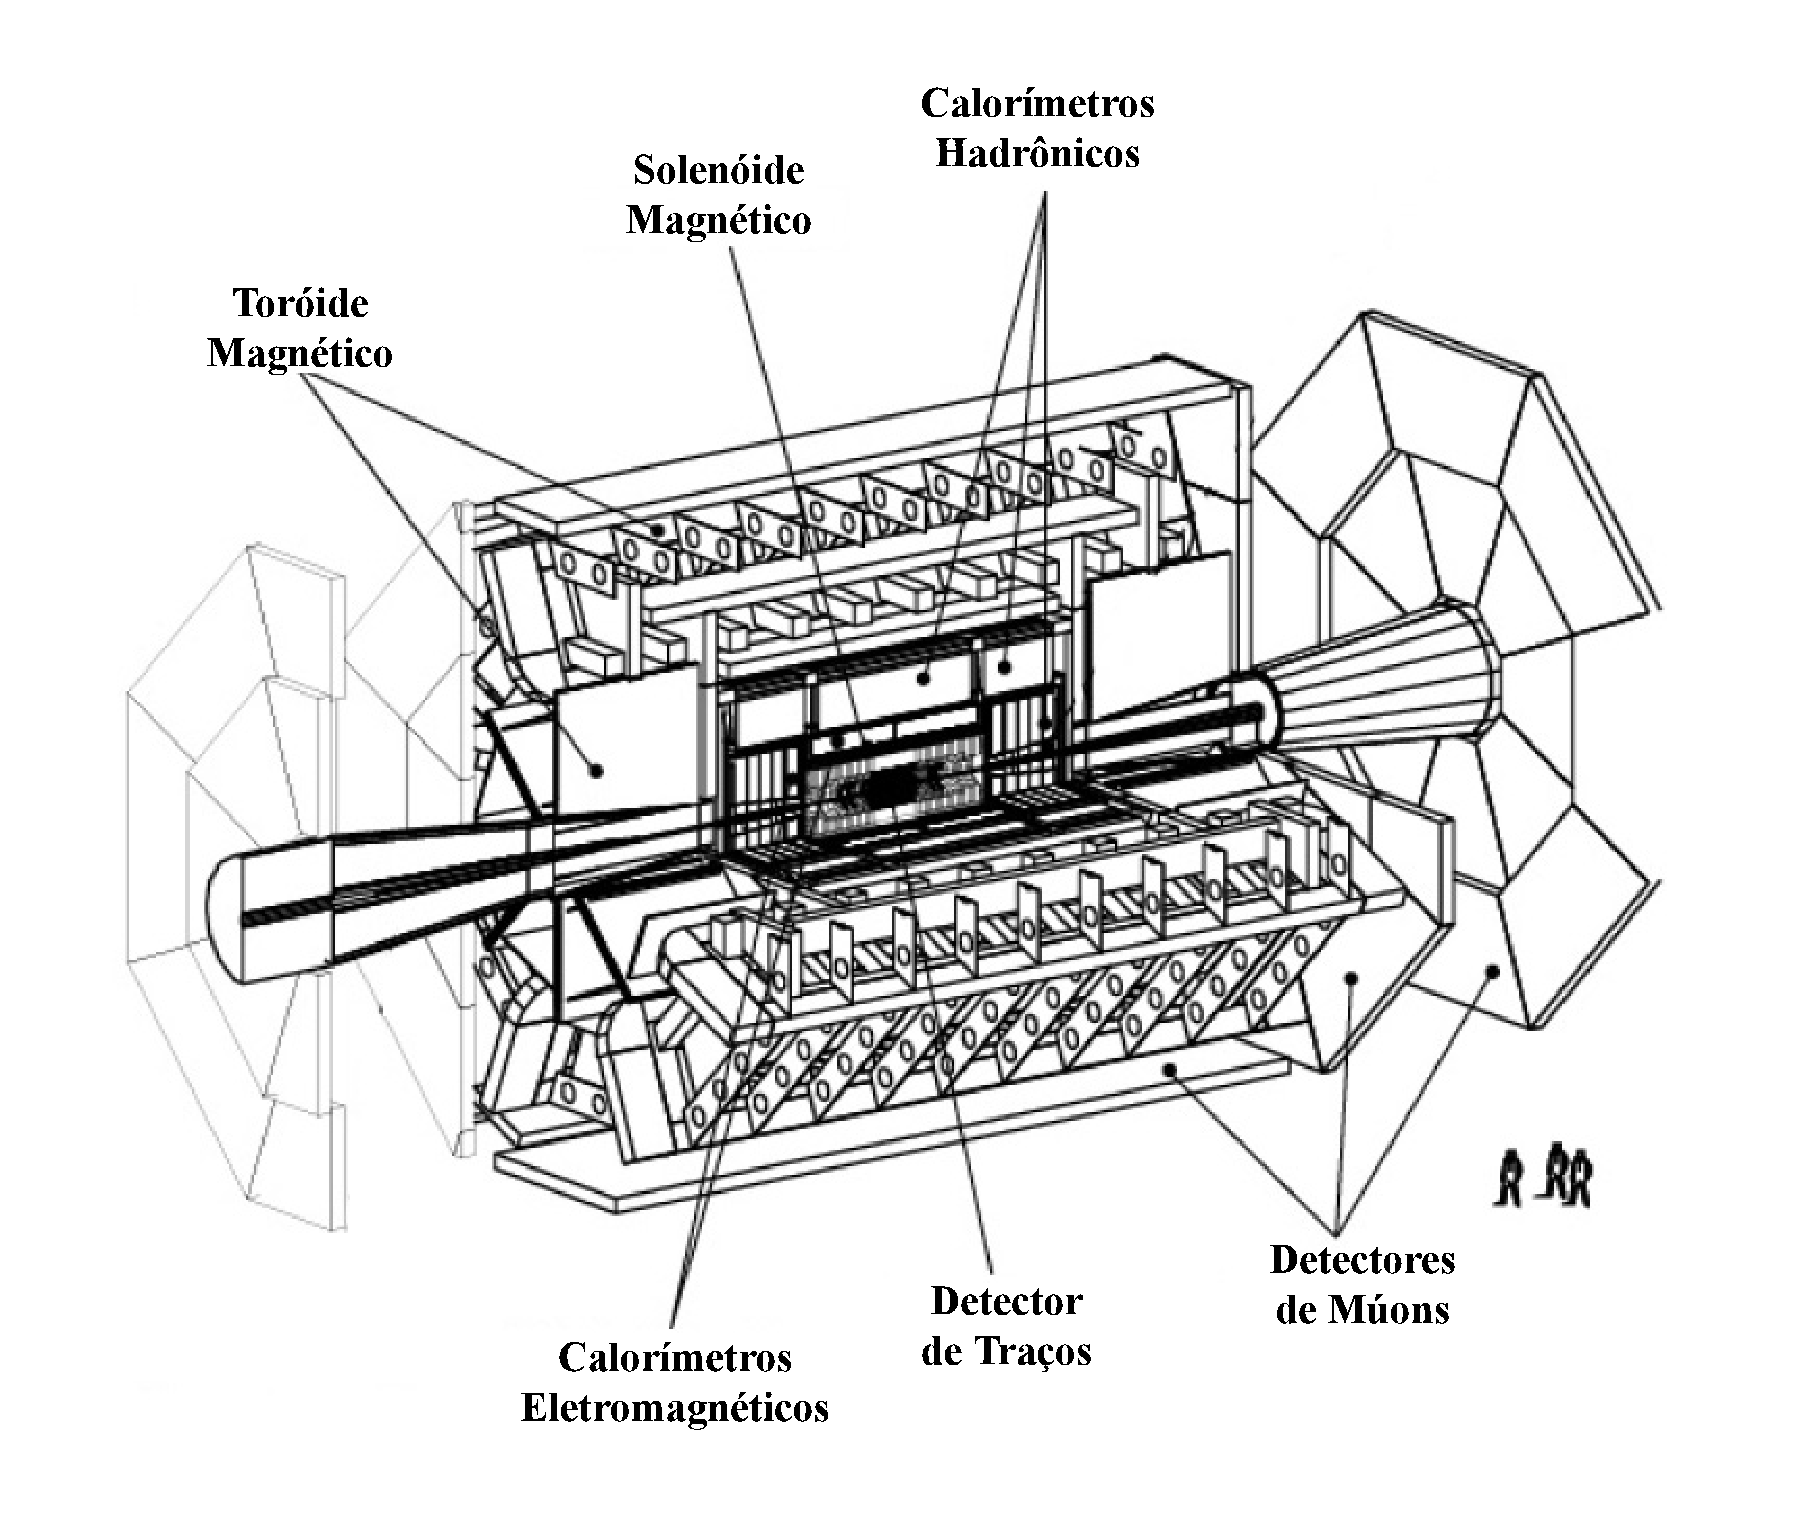
\includegraphics[width=15cm]{cap2_atlas_diag}
\caption{Diagrama esquem�tico do ATLAS.} \label{atlas_diag}
\end{figure}

A fun��o dos detectores de trajet�ria � medir o momento das
part�culas ele\-tri\-camente carregadas, a partir da curvatura de
sua trajet�ria, quando imersos no campo magn�tico do solen�ide
central \cite{atlastracking:2007}. Caminhando do eixo central para
as extre\-mi\-dades, em sequ�ncia, est�o os calor�metros, que medem
a energia depositada pelas part�culas \cite{atlascalo:2002}. Na
intera��o com as c�lulas do calor�metro, s�o produzidos chuveiros de
part�culas secund�rias \cite{book:wigmans:2000}. Num �ltimo est�gio
est� o detector de m�ons, sistema dedicado � detec��o destas
part�culas, que s�o as �nicas que n�o ficam contidas nos
calor�metros \cite{atlasmuon:2004}.

O sistema $xyz$ de coordenadas do ATLAS � �nico para todos os
subsistemas. Conforme mostrado na Figura \ref{atlas_coord}, a
dire��o do feixe do LHC define o eixo $z$, e os eixos $x$ e $y$
formam um plano transverso ao feixe. A dire��o positiva do eixo $x$
� definida apontando do ponto de intera��o para o centro do anel do
LHC, e o eixo $y$ positivo aponta para cima. O �ngulo azimutal �
obtido a partir de:

\begin{equation}\label{phi}
   \phi=\textrm{arctg}(x/y),
\end{equation}
\\
sendo que $\phi=0$ corresponde ao eixo $x$ positivo e $\phi$ aumenta
no sentido hor�rio. O �ngulo polar $\theta$ � medido a partir do
eixo do feixe (eixo $z$ positivo). O momento transverso $p_T$, a
energia transversa $E_T$ e a energia transversa perdida $E_T^{miss}$
s�o definidas no plano $xy$. A pseudo-rapidez $\eta$ � calculada a
partir do �ngulo $\theta$ de es\-pa\-lha\-mento em rela��o ao eixo
$z$ (�ngulo de sa�da das part�culas ap�s a
colis�o)~\cite{LI:ATLAS:1992}:

\begin{figure}[b!] \centering
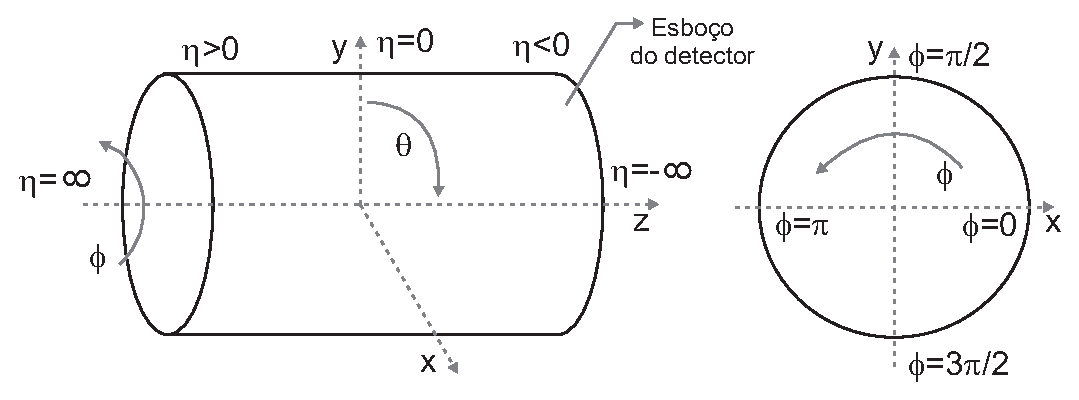
\includegraphics[width=6cm]{cap2_coord}
\caption{Eixo de coordenadas do ATLAS.} \label{atlas_coord}
\end{figure}

\begin{equation}\label{eta}
    \eta=-\ln\textrm{tg}(\theta /2).
\end{equation}
\\
A partir das defini��es das equa��es \ref{phi} e \ref{eta},
define-se o eixo ($\eta,\phi$), onde o �ngulo $\phi$ representa a
rota��o e $\eta$ a dire��o de proje��o das part�culas ap�s a
colis�o. Grandes valores da pseudo-rapidez indicam que a colis�o das
part�culas n�o foi frontal, pois o �ngulo de sa�da, ap�s o choque, �
pequeno, no limite quando $\theta \rightarrow 0$ ent�o $\eta
\rightarrow \infty$. Nesse tipo de colis�o, como quase n�o houve
choque, a produ��o de part�culas elementares � pequena. O ATLAS foi
projetado com baixa resolu��o para $\eta>3$.

\begin{figure}[tbph]
\begin{center}
\subfigure[]{\label{corte1}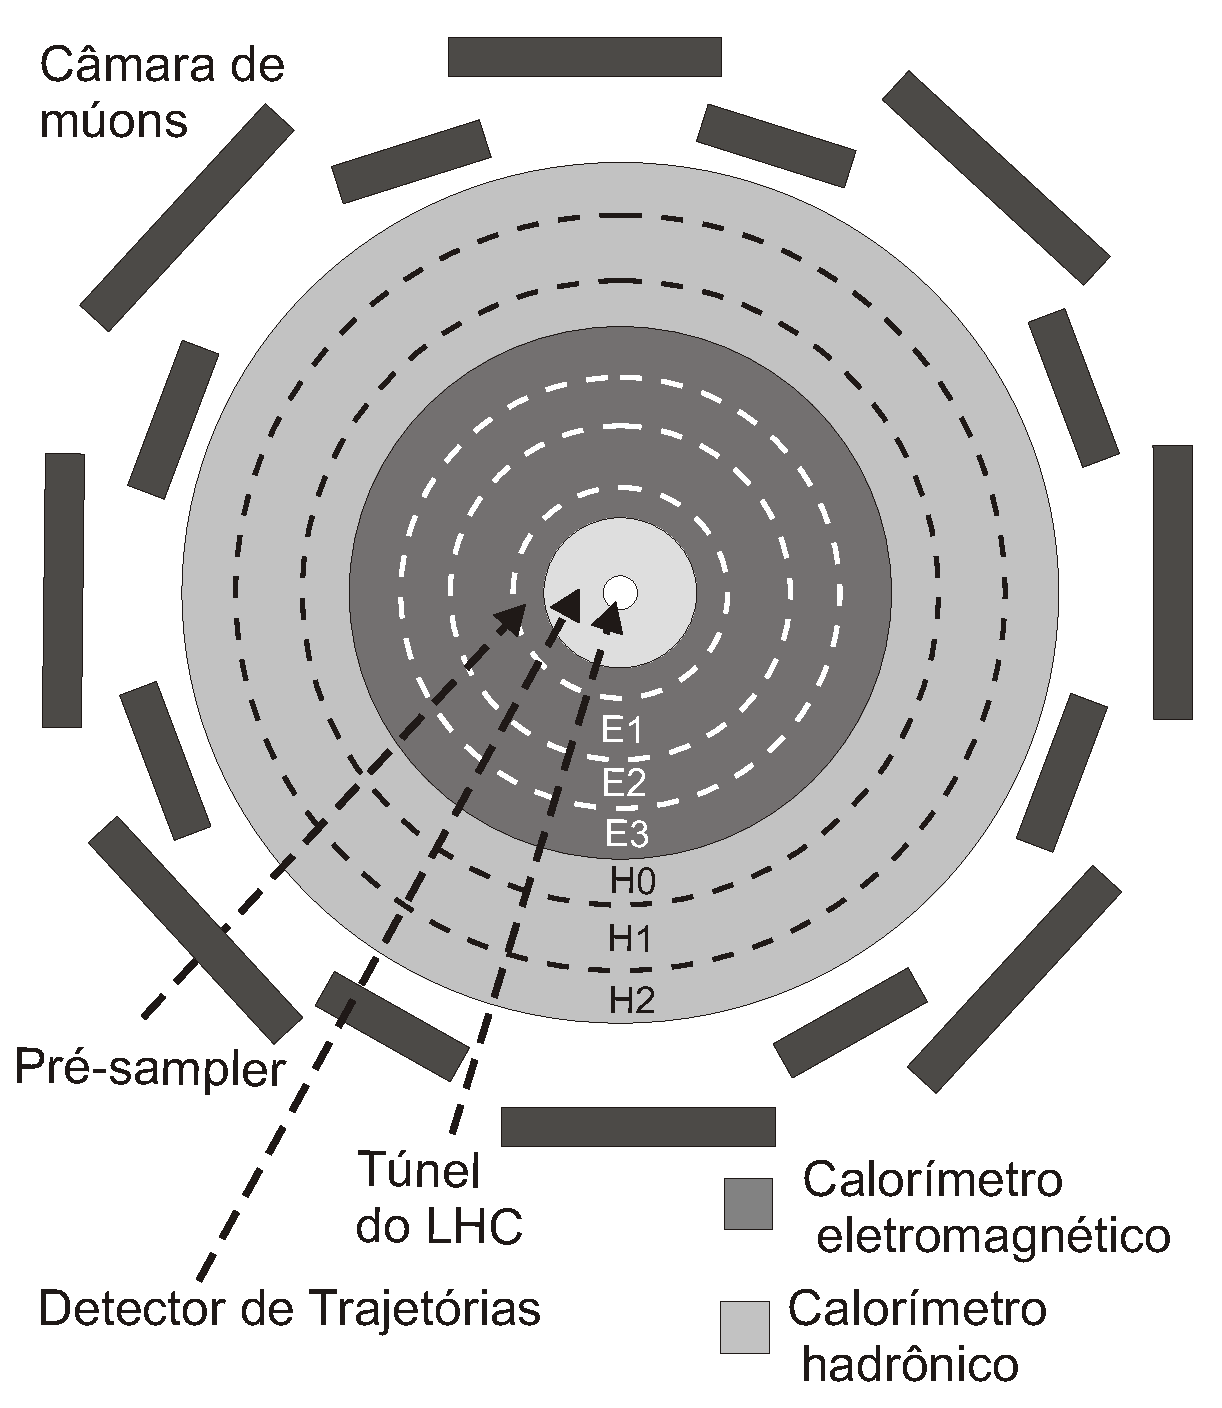
\epsfig{file=cap2_atlas_corte1,width=10cm,clip=}}
\subfigure[]{\label{corte2}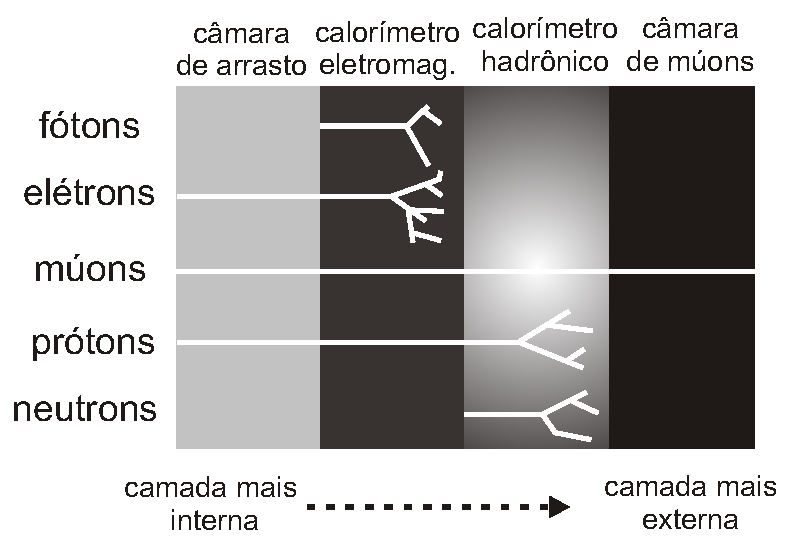
\epsfig{file=cap2_atlas_corte2,width=10cm,clip=}}
\end{center} \caption{Cortes (a) transversal e (b) axial do ATLAS.}
\end{figure}
%, extra�das de \cite{Homepage:ATLAS}

Ap�s uma colis�o, as part�culas geradas interagem com o material do
detector, perdendo energia e consequentemente velocidade. Na Figura
\ref{corte1} pode-se visualizar os subsistemas do ATLAS num corte
transversal (paralelo ao plano $xy$). Percebe-se que a c�mara de
m�ons e o calor�metro hadr�nico t�m as maiores dimens�es. Na figura
\ref{corte2} � mostrada a penetra��o e consequente visualiza��o
esperadas de algumas part�culas nas camadas do detector. N�o
espera-se, por exemplo, deposi��o de energia de f�tons ou el�trons
al�m das camadas eletromagn�ticas do calor�metro, pois estas
part�culas interagem intensamente com os materiais que comp�em a
se��o eletromagn�tica, perdendo toda sua energia. As part�culas
hadr�nicas podem interagir com menos intensidade com o calor�metro
eletromagn�tico e precisam das camadas hadr�nicas para serem
paradas. Os m�ons, em geral, s�o part�culas que perdem pouca energia
nos calor�metros, necessitando de um sistema especial para serem
detectados, o detector de m�ons.

O ATLAS foi projetado e constru�do considerando-se as condi��es
experimentais produzidas pelas colis�es do LHC e com o objetivo de
obter informa��es importantes para responder �s quest�es chave em
f�sica de part�culas. Entre os principais crit�rios utilizados para
o projeto do detector pode-se destacar \cite{article:ATLAS:2008}:

\begin{itemize}
  \item Os elementos sensores e circuitos eletr�nicos devem
  apresentar resposta r�pida e resist�ncia a altos n�veis de
  radia��o. A fina granularidade do detector � importante para
  reduzir a influ�ncia dos eventos sobrepostos.

  \item Excelente calorimetria eletromagn�tica para a identifica��o de
el�trons e f�tons, complementada por informa��es acuradas dos
calor�metros hadr�nicos, para medi��es de jatos hadr�nicos e energia
transversa $E_T$ (se o valor para $E_T$ for diferente do esperado
isso pode indicar a ocorr�ncia de um fen�meno n�o observado pelo
detector);

  \item Eficiente sistema de identifica��o de trajet�ria para medi��o do
momento;

  \item Alta precis�o na identifica��o de m�ons;

  \item Alta aceita��o em pseudo-rapidez ($\eta$) com cobertura quase total no
�ngulo azimutal ($\phi$);

  \item Alta efici�ncia do sistema de filtragem (\textit{trigger}),
armazenando a maioria dos eventos f�sicos de interesse e reduzindo
ao m�ximo o ru�do de fundo (informa��o n�o relevante) produzido nas
colis�es do LHC.
\end{itemize}

Conforme mencionado no Cap�tulo 1, o estudo conduzido neste trabalho
utiliza informa��es do sistema de calor�metros do ATLAS e prop�e
algoritmos para a otimiza��o da detec��o (trigger) de el�trons. Nas
pr�ximas sub-se��es, ser�o des\-cri\-tos o sistema de calor�metros
do ATLAS e a import�ncia da detec��o de el�trons para o desempenho
do experimento.

\subsection{O sistema de calorimetria do ATLAS}

Calor�metros \cite{book:wigmans:2000} representam uma importante
classe de detectores para medi��o de energia e posi��o da part�cula.
Durante o processo de absor��o, as part�culas interagem com o
material dos calor�metros gerando part�culas secund�rias que, por
sua vez, interagem tamb�m gerando outras part�culas e assim por
diante. Este processo � chamado de cascata ou chuveiro de
part�culas. Os calor�metros podem apresentar resposta muito r�pida,
da ordem de nanosegundos \cite{book:wigmans:2000}, e, por isso, �
utilizado intensamente pelo sistema de filtragem online
(\textit{trigger}). As prov�veis classes de part�culas s�o
identificadas a partir das caracter�sticas esperadas para o seu
perfil de deposi��o de energia.

Calor�metros s�o detectores de absor��o total. O processo de medi��o
utilizado � destrutivo e as part�culas n�o est�o dispon�veis ap�s a
passagem pelos calor�metros (com excess�o aos m�ons, que conseguem
penetrar em grande quantidade de mat�ria e necessitam de um detector
especial a c�mara de m�ons). Quando part�culas atravessam mat�ria,
elas em geral interagem e perdem assim uma parte de sua energia.
Neste processo o meio � excitado ou aquecido (da� o termo
calorimetria). Na pr�tica absor��o ``total" significa 99 a 99,9 $\%$
da energia (ou at� um pouco menos). A depender do tipo de part�cula
e da energia envolvida, a part�cula pode exceder os limites do
calor�metro (vazar) e acabam por interferir em outros detectores
(ex. c�mara de m�ons) \cite{book:wigmans:2000}.

Os calor�metros podem ser classificados em homog�neos ou
amostradores. No calor�metro homog�neo todo o volume do detector �
sens�vel �s part�culas e contribuem para produ��o do sinal, no
calor�metro amostrador o material passivo absorve (interage) as
part�culas e o material ativo produz o sinal
\cite{book:wigmans:2000}.

Part�culas como el�trons e p�sitrons interagem com a mat�ria gerando
um chuveiro de part�culas menos energ�ticas e necessitam de pequena
quantidade de material para serem totalmente absorvidas. Os m�ons,
por outro lado, perdem sua energia muito lentamente necessitando de
grande quantidade de mat�ria para a absor��o total. As part�culas
hadr�nicas interagem com a mat�ria atrav�s da for�a nuclear forte. O
processo de intera��o � muito mais complexo que o EM e uma variedade
muito grande de fen�menos pode ocorrer. Os hadrons podem, por
exemplo, se comportar de modo semelhante a el�trons e m�ons, ou se
envolverem em uma intera��o nuclear e se transformarem em 15 novos
h�drons. Uma parte da energia das intera��es hadr�nicas n�o �
vis�vel (detect�vel) pelos calor�metros pois os hadrons neutros n�o
ionizam o calor�metro e a energia � perdida em intera��es nucleares
(fundamentalmente n�o detectadas pelo calor�metro)
\cite{book:wigmans:2000}.

Os calor�metros deveriam ser intrinsecamente lineares para a
detec��o de part�culas EM. Por exemplo um par de el�trons de 10 GeV
deveria gerar um sinal de mesma intensidade que um �nico el�tron de
20 GeV. Na pr�tica, desvios do comportamento linear (para part�culas
EM) podem ser observados na pr�tica devido a fen�menos como
\cite{book:wigmans:2000}:
\begin{itemize}
    \item Satura��o das foto-multiplicadoras (PMT - \textit{Photo-Multipliers}) - as PMT convertem luz dos calor�metros cintiladores em sinais el�tricos, sua satura��o implica em distor��o n�o-linear dos sinais el�tricos;
    \item Vazamento do chuveiro - com o aumento da energia algumas part�culas podem extrapolar os limites do detector, havendo, neste caso, perda de parte da informa��o;
    \item Recombina��o dos el�trons com �ons do material ativo - se isso ocorrer a ioniza��o n�o � detectada;
    \item Atenua��o da luz - a luz emitida pelo material ativo (cintilante) pode ser atenuada antes de atingir as PMT.
\end{itemize}

Calor�metros homog�neos s�o intrinsecamente n�o-lineares para a
detec��o de hadrons e jatos. A fra��o EM de chuveiros hadr�nicos
depende da energia e varia bastante de evento para evento, tornando
a resposta hadr�nica n�o-constante em fun��o da energia (tanto para
calor�metros homog�neos como para os amostradores). A fra��o n�o EM
(que produz intera��es nucleares) �, em geral, menor. Em qualquer
calor�metro a resolu��o em energia para h�drons � pior que para
el�trons de mesma energia. Isso se deve ao fato de ocorrerem
flutua��es na energia vis�vel (detect�vel) aos calor�metros
\cite{book:wigmans:2000}.

Como as caracter�sticas dos chuveiros eletromagn�ticos e hadr�nicos
s�o di\-fe\-ren\-tes, na pr�tica, s�o utilizados tipos de
calor�metro espec�ficos para estas classes de part�culas
\cite{book:martin:2006}. O calor�metro eletromagn�tico � usualmente
instalado internamente ao hadr�nico. As part�culas eletromagn�ticas
(ex: el�trons e f�tons) apresentam perfil de deposi��o de energia
que, em geral, � concentrado em torno do ponto de colis�o.
Tipicamente, as part�culas eletromagn�ticas s�o absorvidas
completamente nos calor�metros eletromagn�ticos. Os chuveiros
hadr�nicos apresentam formas va\-ria\-das e iniciam sua intera��o
com o calor�metro eletromagn�tico, mas, em geral, somente s�o
completamente absorvidas nas camadas hadr�nicas (mais externas).

O sistema de calor�metros do detector ATLAS
\cite{article:ATLAS:2008} � sub-dividido em 7 camadas
\cite{atlascalo:2002}, sendo 4 eletromagn�ticas (PS, E1, E2, E3) e 3
hadr�nicas (H0, H1 e H2), conforme Figura \ref{atlas_calo}. Cada
camada apresenta diferente concentra��o de c�lulas detectoras por
unidade de �rea (granularidade). O calor�metro eletromagn�tico (EM)
� composto de finas folhas de chumbo separadas por dispositivos
sensores de arg�nio l�quido, cobrindo a regi�o onde $|\eta|<3,2$. As
tr�s camadas do calor�metro eletromagn�tico s�o divididas em barril
(regi�o central do detector, onde $|\eta|<1,5$) e tampa (regi�es
mais externas onde $1,4<|\eta|<3,2$). Na regi�o onde $|\eta|<1,8$,
imediatamente antes da primeira camada EM existe uma fina camada de
arg�nio l�quido chamada pr�-amostrador (\textit{presampler} ou PS).
O pr�-amostrador � importante para corrigir medi��es nas quais
existe perda de energia no caminho at� os calor�metros.

Um problema espec�fico do ATLAS � o substancial volume de material
inerte(morto) instalado entre o ponto de colis�o e os calor�metros.
O pr�-amostrador tem fun��o prim�ria amenizar os problemas causados
pela perda de energia neste material (em 119 GeV ~5$\%$ da energia
de el�trons � perdida neste material). Os sinais medidos no PS s�o
ponderados por um fator adequado $\alpha$ e somados aos sinais
medidos nas outras camadas para compor a energia total do evento
\cite{book:wigmans:2000}:
\begin{equation}\label{ps}
E_{tot} = E_{calo} + \alpha E_{ps}.
\end{equation}

O calor�metro hadr�nico envolve o eletromagn�tico. Na regi�o onde
$|\eta|<1,7$, ele � composto de placas absorvedoras de a�o separadas
por telhas de material pl�stico cintilante. Quando as part�culas
atravessam as telhas elas emitem luz de intensidade proporcional �
energia incidente \cite{TDR1:ATLAS:1999}. O sinal luminoso � ent�o
convertido em el�trico atrav�s de placas foto-multiplicadoras. Esta
parte do calor�metro hadr�nico do ATLAS � conhecida como calor�metro
de telhas (\textit{Tile Calorimeter} ou simplesmente
\textit{TileCal}) e � dividida em barril ($|\eta|<1,0$) e
barril-extendido ($0,8<|\eta|<1,7$) \cite{article:tilecal:2006}.
Para a tampa do calor�metro hadr�nico ($|\eta|>1,5$) utiliza-se a
tecnologia do arg�nio l�quido.

\begin{figure}[h]
\centering
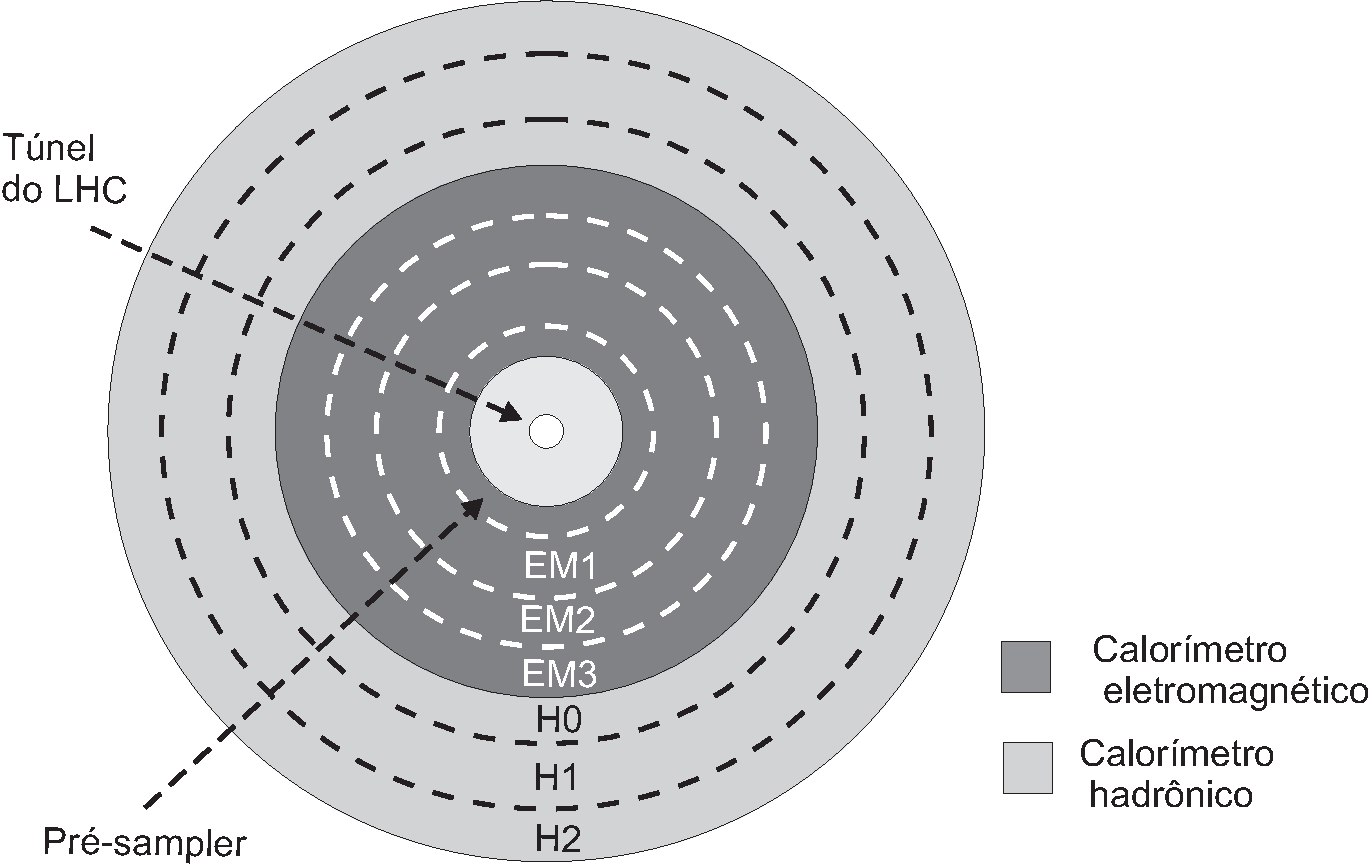
\includegraphics[width=11cm]{cap2_calo}
\caption{Disposi��o em camadas dos calor�metros do ATLAS.}
\label{atlas_calo}
\end{figure}

A informa��o da energia depositada nas camadas do calor�metro, com
fina segmenta��o, � muito importante para a caracteriza��o f�sica
das part�culas. Ap�s um evento ser aceito pelo sistema de filtragem,
todas as informa��es relativas a este evento s�o armazenadas em
m�dia permanente para posterior an�lise \textit{off-line}. A
granularidade, ou quantidade de c�lulas por unidade de �rea, varia
entre as camadas do calor�metro. A Tabela \ref{tab_calo} traz
informa��es sobre a regi�o de cobertura em $\eta$, granularidade e
quantidade de canais de leitura (c�lulas sensoras) de cada camada do
calor�metro.

\begin{table}[t!]
\centering
\caption{Regi�o de cobertura em $\eta$, granularidade e n�mero de
canais de leitura das camadas dos calor�metros.} \vspace{.3cm}
\begin{tabular}{l c c}
  \hline
  \hline
  % after \\: \hline or \cline{col1-col2} \cline{col3-col4} ...
  \textbf{Pre-amostrador}    & \textbf{Barril}  & \textbf{Tampa}  \\  \hline
  Cobertura   &  $|\eta|<1,52$ & $1,5<|\eta|<1,8$   \\
  Granularidade ($\Delta \eta \times \Delta \phi$)    &  $0,025 \times 0,1$ & $0,025 \times 0,1$  \\
  Canais de Leitura & 7808 & 1536 (ambos os lados)\\
  \hline
  \hline
  \textbf{Eletromagn�tico}    & \textbf{Barril}  & \textbf{Tampa}  \\  \hline
  Cobertura   &  $|\eta|<1,475$ & $1,375<|\eta|<3,2$   \\
  Granularidade ($\Delta \eta \times \Delta \phi$)& &  \\
  Camada 1      &  $0,025/8 \times 0,1$ & $0,025/8 \times 0,1$ a $0,1 \times 0,1$  \\
  Camada 2      &  $0,025 \times 0,025$ & $0,025 \times 0,025$ a  $0,1 \times 0,1$  \\
  Camada 3      &  $0,050 \times 0,025$ & $0,05 \times 0,025$   \\
  Canais de Leitura & 101760 & 62208 (ambos os lados)\\
   \hline
   \hline
  \textbf{Had. Telhas Cintilantes}    & \textbf{Barril}  & \textbf{Barril estendido}     \\  \hline
  Cobertura   &  $|\eta|<1,0$ & $0,8<|\eta|<1,7$   \\
  Granularidade ($\Delta \eta \times \Delta \phi$)& &  \\
  Camadas 1, e 2    &  $0,1 \times 0,1$ & $0,1 \times 0,1$   \\
  Camada 3   &  $0,2 \times 0,1$ & $0,2 \times 0,1$   \\
  Canais de Leitura & 5760 & 4092 (ambos os lados)\\
  \hline
     \hline
  \textbf{Had. Arg�nio L�quido}    & \textbf{Tampa}  &      \\  \hline
  Cobertura   &  $1,5<|\eta|<3,2$  &  \\
  Granularidade ($\Delta \eta \times \Delta \phi$)& &  \\
  Camadas 1, 2 e 3    &  $0,1 \times 0,1$ a $0,2 \times 0,2$ &  \\
  Canais de Leitura & 5632 (ambos os lados)& \\
  \hline
  \hline
\end{tabular}
\label{tab_calo}
\end{table}
%, extra�da de \cite{article:ATLAS:2008}

Conforme ilustrado na Figura \ref{calo_cell}, percebe-se que a
primeira camada eletromagn�tica apresenta mais fina segmenta��o,
possibilitando medi��o precisa do ponto de colis�o. A segunda camada
apresenta c�lulas detectoras quadradas e maior profundidade,
absorvendo maior parcela da energia. A terceira camada, por sua vez,
captura os detalhes do final do chuveiro eletromagn�tico.

\begin{figure}[h]
\centering
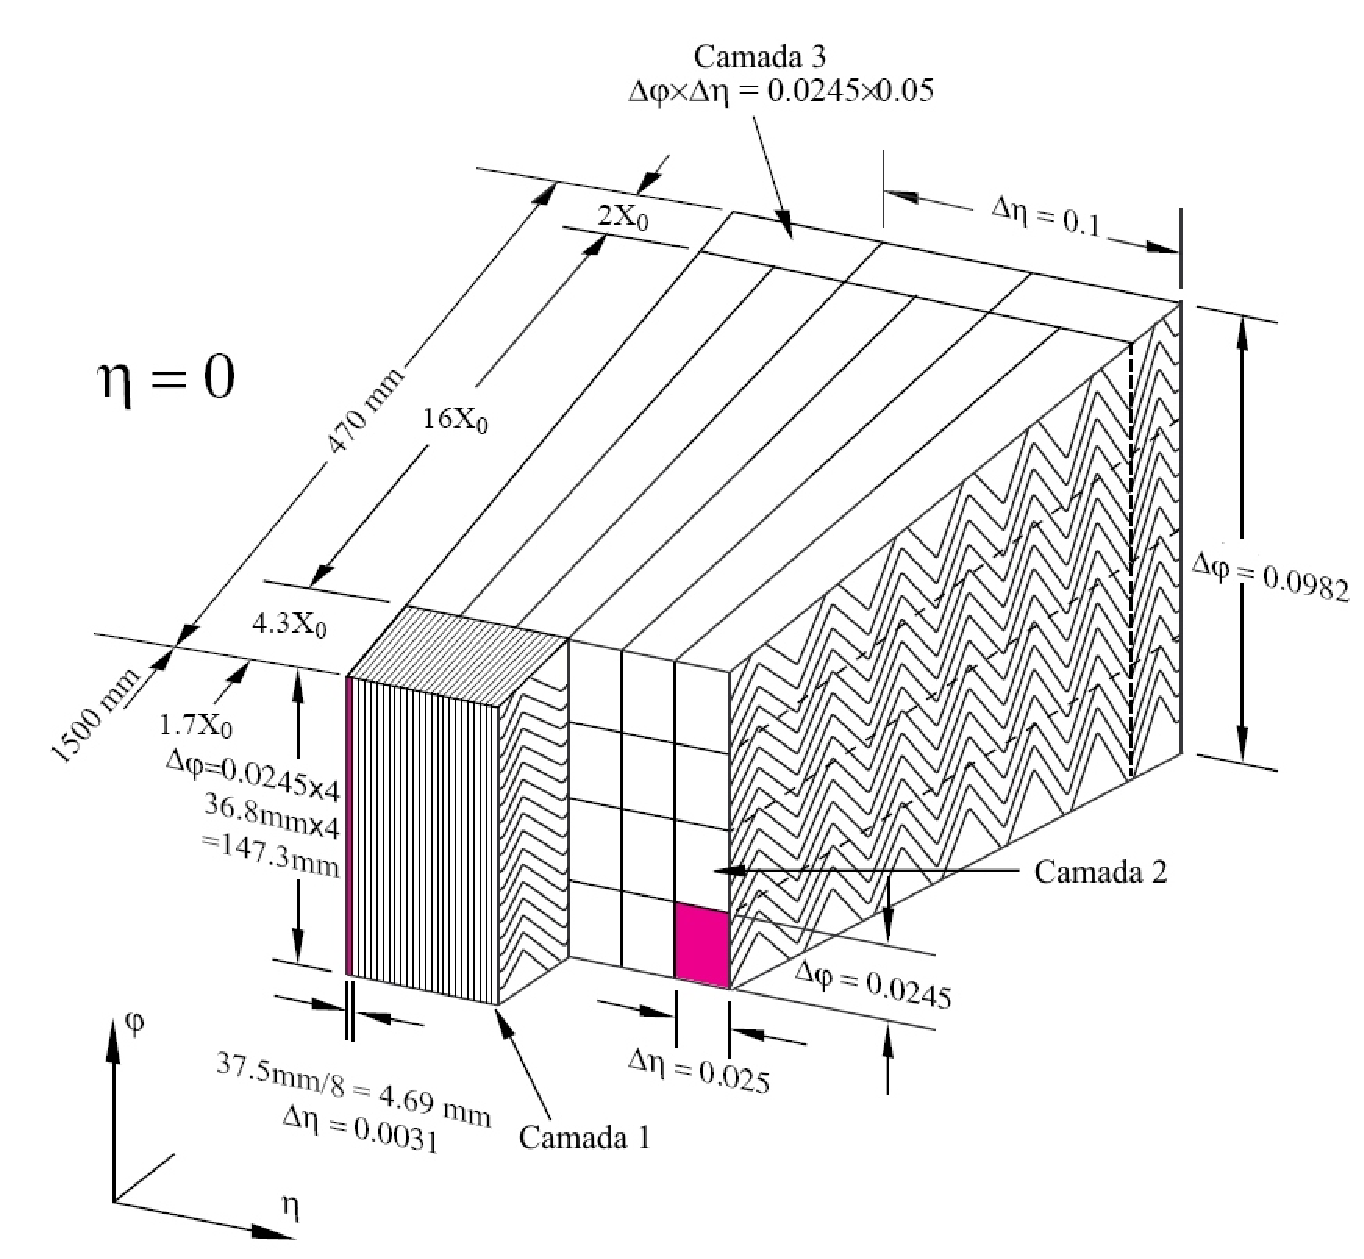
\includegraphics[width=13cm]{cap2_caloem}
\caption[Granularidade e profundidade das camadas do calor�metro
eletromagn�tico.]{Granularidade e profundidade das camadas do calor�metro
eletromagn�tico, extra�do de \cite{article:ATLAS:2008}.}
\label{calo_cell}
\end{figure}
%, adaptada de \cite{article:ATLAS:2008}

Calor�metros s�o constru�dos utilizando estruturas modulares. Os
cabos de transmiss�o de sinais e alimenta��o passam por espa�os
existentes entre os m�dulos (\textit{cracks}). No ATLAS, na regi�o
de $|\eta|\sim 1,5$ (interconex�o entre barril e barril-extendido)
existe uma descontinuidade nos calor�metros (eletromagn�tico e
hadr�nico) para passagem de cabos de alimenta��o e dados do detector
de trajet�ria e do barril do calor�metro eletromagn�tico
\cite{article:ATLAS:2008}. Nesta faixa, h� menor quantidade de
c�lulas detectoras e, consequentemente, baixa resolu��o nas medi��es
obtidas (o que pode representar um problema para o sistema de
filtragem, como ser� descrito na Se��o \ref{sec_trig}).

Diferente de outros tipos de detectores, a precis�o dos calor�metros
aumenta com a energia \cite{book:wigmans:2000}:
\begin{equation}\label{res_calo}
    \frac{\sigma_E}{E} \propto \frac{1}{\sqrt{E}}
\end{equation}
onde E � a energia incidente por part�cula e $\sigma_E$ a varia��o (desvio padr�o) esperado na medi��o. Outras fontes de
flutua��es de menor import�ncia contribuem com fatores de outra
ordem como ru�do eletr�nico: $\propto 1/E$ (domina em baixa energia,
principalmente em calor�metros de Arg�nio L�quido - LAr); e vazamento lateral do chuveiro: $ \propto
1/(E)^{1/4}$. Existem ainda flutua��es que s�o independentes da energia. Uma caracter�stica interessante � que as flutua��es
podem n�o ser sim�tricas em torno do valor m�dio. Um estudo detalhado a respeito das flutua��es encontradas em calor�metros pode ser encontrado em \cite{book:wigmans:2000}.

Para o calor�metro do ATLAS, foi calculada experimentalmente
em~\cite{atlascalo:2002} a resolu��o esperada . Os valores
encontrados foram $0,1/\sqrt{E}$ e $0,4/\sqrt{E}$, respectivamente
para os calor�metros eletromagn�tico (de arg�nio l�quido) e
hadr�nico (de telhas cintilantes).

%Um fato que ser� freq�ente durante o tempo de opera��o do detector �
%a da\-ni\-fi\-ca��o de c�lulas. Devido � alta intensidade de energia
%produzida pelas colis�es, algumas regi�es podem ser danificadas,
%deixando de registrar corretamente as informa��es de energia
%depositada, e at� parando totalmente de funcionar
%\cite{TP:ATLAS:1994}. Os algoritmos de filtragem de eventos devem
%ter alguma imunidade � perda de informa��o das c�lulas.

\subsection{Principais objetos de interesse no ATLAS}

Dentre os eventos gerados nas colis�es do LHC, apenas uma pequena
parte ser� �til para a caracteriza��o dos processos da ``nova
f�sica". Com o LHC operando em alta luminosidade podem ocorrer at�
10$^9$ intera��es por segundo, por�m, os eventos de interesse s�o
muito raros. Por exemplo a depender de sua massa, a taxa de ocorr�ncia do b�son de Higgs pode variar de 0,01 a 0,1 Hz e eventos de supersimetria s�o esperados a 1 Hz~\cite{article:trigconf:2009}

Provar a exist�ncia do b�son de Higgs � um dos principais objetivos
do LHC. Com o conhecimento adquirido at� agora, n�o � poss�vel
determinar sua massa $m_H$, embora seu limite inferior ($m_H>114$
GeV/c$^2$) tenha sido determinado pelos resultados obtidos em outros
aceleradores, como o LEP (\textit{Large Electron Positron Collider},
acelerador que operou no CERN de 1989 a 2000) \cite{drees:lep:2001}.
O limite superior esperado por estudos te�ricos � $\sim$ 1 TeV/c$^2$
\cite{book:lhc:2008}.

Considerando os diversos decaimentos poss�veis para a part�cula de
Higgs, espera-se que o canal mais limpo para seu estudo aconte�a se
sua massa estiver aproximadamente na faixa 150$<m_H<$700 GeV/c$^2$
\cite{article:ATLAS:2008}. Neste caso, o Higgs pode apresentar o
decaimento em 2 b�sons Z, com cada Z, por sua vez,
decaindo\footnote{No decaimento de part�culas elementares, parte da
massa da part�cula � convertida em energia e o restante em massa de
outras part�culas} em dois l�ptons (el�trons ou m�ons):
\begin{equation}\label{higgs_dec}
    H \rightarrow ZZ^{(*)} \rightarrow l^+ l^- l^+ l^-
\end{equation}

Para este canal de busca do Higgs, � fundamental que os detectores
tenham um sistema de filtragem capaz de identificar com alta
efici�ncia el�trons e m�ons. Estas duas part�culas, assim como os
f�tons, jatos e os taus, s�o importantes tamb�m para o melhor
entendimento da supersimetria (SUSY - \emph{supersimetry})
\cite{livro:fisica1:2006}. Os taus tamb�m podem levar aos modelos de
Higgs estendidos \cite{TDR2:ATLAS:1999}. Um resumo com os principais
objetos de interesse no ATLAS e suas aplica��es na f�sica � mostrado
na Tabela \ref{tab_fisica}.

\begin{table}[h!]
\centering
\caption[Principais objetos de interesse no ATLAS.]{Principais objetos de interesse no ATLAS, extra�da de
\cite{article:HLT1:2003}.}\vspace{.3cm}
\begin{tabular}{c c }
  \hline
  % after \\: \hline or \cline{col1-col2} \cline{col3-col4} ...
  \textbf{Objeto}    & \textbf{F�sica de interesse}       \\  \hline
  \textbf{El�tron}   &  Higgs, SUSY, dimens�es-extra, novos b�sons e \textit{top quark}\\
  \textbf{F�ton}    &  Higgs, SUSY e dimens�es-extra\\
  \textbf{M�on}      & Higgs, SUSY, extra-dimens�es, novos b�sons e \textit{top quark}\\
  \textbf{Jato}   &  SUSY e resson�ncias\\
  \textbf{Jato + $E_T^{miss}$}    &SUSY e \textit{leptoquarks}\\
  \textbf{Tau + $E_T^{miss}$}      & Modelo de Higgs estendido e SUSY\\
  \hline
\end{tabular}
\label{tab_fisica}
\end{table}
%, extra�da de \cite{article:HLT1:2003}book:montecarlo:2004

A identifica��o \textit{online} destes objetos dentro de um universo
enorme de informa��es � realizada pelo sistema de filtragem
(\textit{trigger}). Conforme mencionado, um dos objetos de interesse
na filtragem do ATLAS � o el�tron. Para a identifica��o de el�trons,
a informa��o obtida no sistema de calor�metros � muito importante.
Em termos da calorimetria, as assinaturas de el�trons podem ser
confundidas com perfis de energia gerados por alguns jatos
hadr�nicos (espacialmente concentrados nas camadas eletromegn�ticas
e com pouca energia nas hadr�nicas). Considerando que a produ��o de
jatos ser� muito frequente nas colis�es do LHC, estes formar�o um
intenso ru�do de fundo para a identifica��o de el�trons. Pelo que
foi exposto, percebe-se que a discrimina��o el�tron/jato (e$^-$/j) �
importante para o desempenho do detector.

    \chapter{Detec��o de El�trons a partir de Informa��es de Calorimetria no ATLAS}

Neste cap�tulo ser�o descritos os principais aspectos do processo de filtragem \textit{online} de el�trons no 
detector ATLAS. O conhecimento adequado da energia de el�trons e f�tons em uma larga faixa (de alguns GeV a 
poucos TeV) � necess�rio para medi��es precisas de fen�menos n�o descritos pelo modelo padr�o e para a busca 
pela part�cula de Higgs no decaimento H$\rightarrow$ZZ*$\rightarrow$4e. A sele��o de el�trons � tamb�m muito 
importante para os processos de calibra��o e alinhamento do detector durante a fase inicial de opera��o. Com 
a an�lise de eventos conhecidos (como por exemplo o decaimento Z$\rightarrow$ee) pode-se gerar informa��es 
valiosas para o melhor conhecimento das caracter�sticas do detector \cite{article:imphlttrigeer:2006}. A 
discrimina��o destas part�culas � baseada nas informa��es do sistema de calor�metros. Considerando informa��es 
do perfil de deposi��o de energia medido nos calor�metros, os el�trons podem ser confundidos com jatos hadr�nicos 
(que neste caso representam ru�do de fundo para o experimento). No LHC, a gera��o de jatos ser� bastante intensa 
(por exemplo, para energia de 40 GeV a rela��o de produ��o el�tron/jato � da ordem de 
10$^{-5}$~\cite{article:ATLAS:2008}) o que tornar� dif�cil a identifica��o da f�sica de interesse. 
Tradicionalmente,a identifica��o de el�trons � realizada analisando-se o formato transversal do chuveiro e o 
vazamento para as camadas hadr�nicas \cite{article:egtrigeer:2006}. Estes par�metros variam com a energia da 
part�cula e nem sempre s�o capazes de produzir alta efici�ncia de discrimina��o.

\section{Desempenho esperado dos calor�metros}

Devido a limita��es construtivas, a precis�o nas medi��es dos calor�metros do ATLAS varia com a 
energia e a posi��o de intera��o. Uma caracter�stica particular do ATLAS � a grande quantidade 
de material instalado entre o ponto de colis�o e o sistema de calor�metros, que provoca severas perdas na medi��o da 
energia de el�trons, conforme mostrado na Figura \ref{cap3_fig_enloss}. 

\begin{figure}[h!] \centering
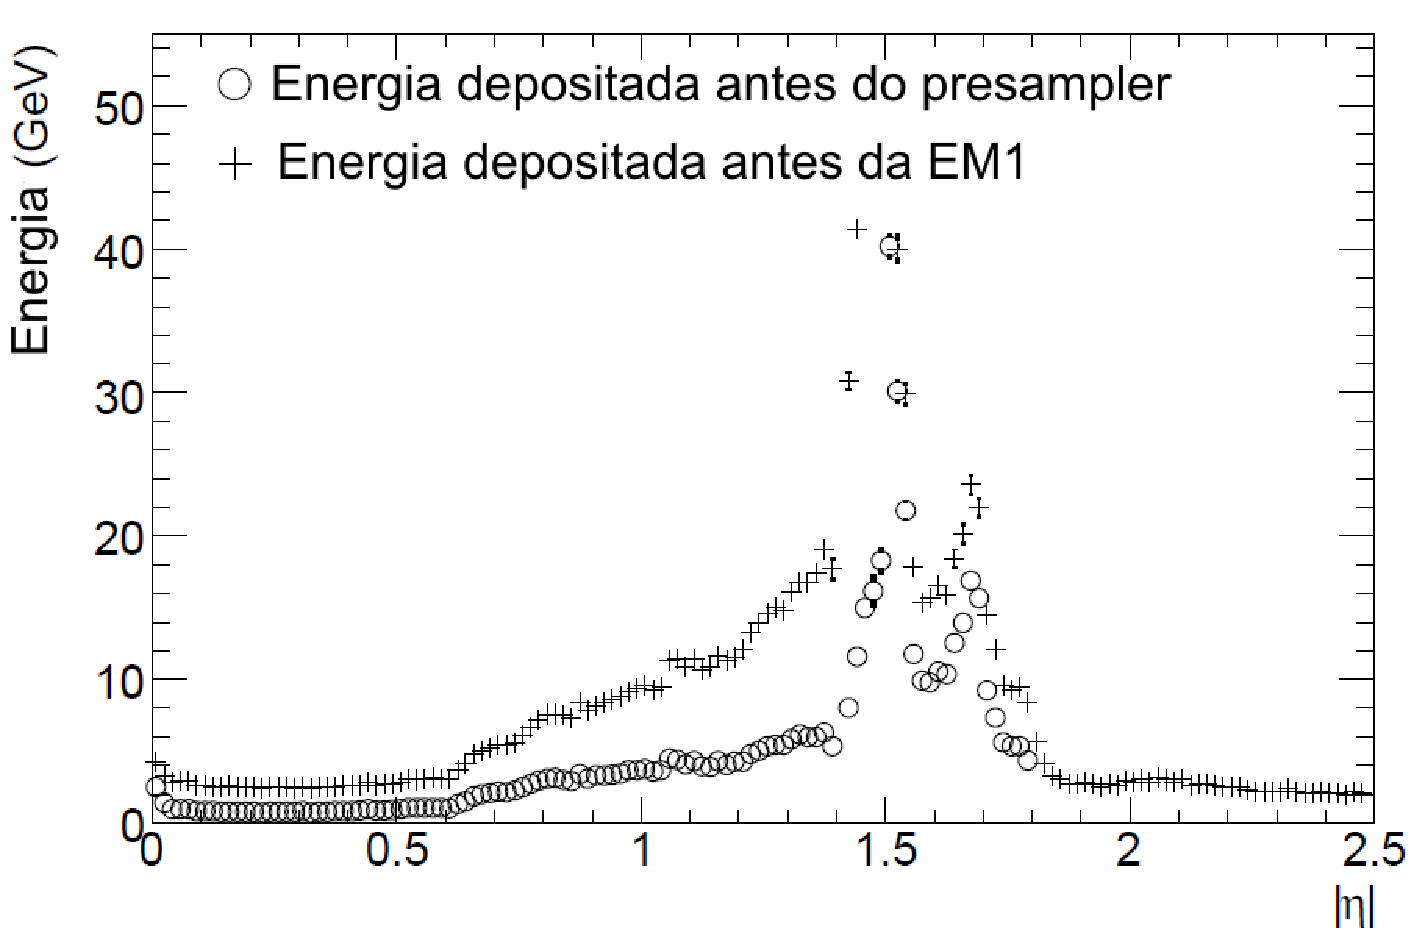
\includegraphics[width=9cm]{cap3_enperdida}
\caption[Energia perdida por el�trons antes do calor�metro.]{Energia perdida por el�trons antes do calor�metro, adaptado de~\cite{article:ATLAS:2008}.} \label{cap3_fig_enloss}
\end{figure}

Numa tentativa de corrigir as medi��es de energia, fatores de pondera��o dependentes de $\eta$ s�o utilizados na 
estimativa da energia total do evento~\cite{article:ATLAS:2008}:
\begin{equation}
 E=s(\eta)[c(\eta)+w_0(\eta).E_{PS}+E_{EM1}+E_{EM2}+w_3(\eta).E_{EM3}]
\end{equation}
sendo $s$ um fator global de corre��o, $c$ uma tend�ncia (ou \textit{bias}), $w_0$ corrige a energia perdida antes do 
calor�metro e $w_3$ corrige o vazamento longitudinal de energia, os termos $E_{PS}$, $E_{EM1}$, $E_{EM2}$ e $E_{EM3}$ 
representam a energia medida em cada camada do calor�metro eletromagn�tico (\textit{presampler}, primeira, segunda e 
terceira camadas eletromagn�ticas).

Os erros relativos ($\frac{\sigma_E}{E}$) esperados em fun��o da energia e de $\eta$ para assinaturas de el�trons 
s�o mostrados na Figura \ref{cap3_enres}. Devido a caracter�sticas construtivas do detector, na 
regi�o de transi��o entre o barril e a tampa do calor�metro 
(entre $\eta=1.37$ e $\eta=1.52$, conhecido como \textit{crack}), a resolu��o da energia � bastante 
degradada. Percebe-se que a precis�o diminui para baixa energia e pr�ximo ao 
\textit{crack} ($\eta \approx 1.5$). Sempre que o erro de medi��o aumenta, a caracteriza��o das part�culas 
� prejudicada, provocando queda de desempenho dos algoritmos de filtragem de el�trons.

\begin{figure}[h!]
\begin{minipage}[b]{.48\linewidth}
  \centering
 \centerline{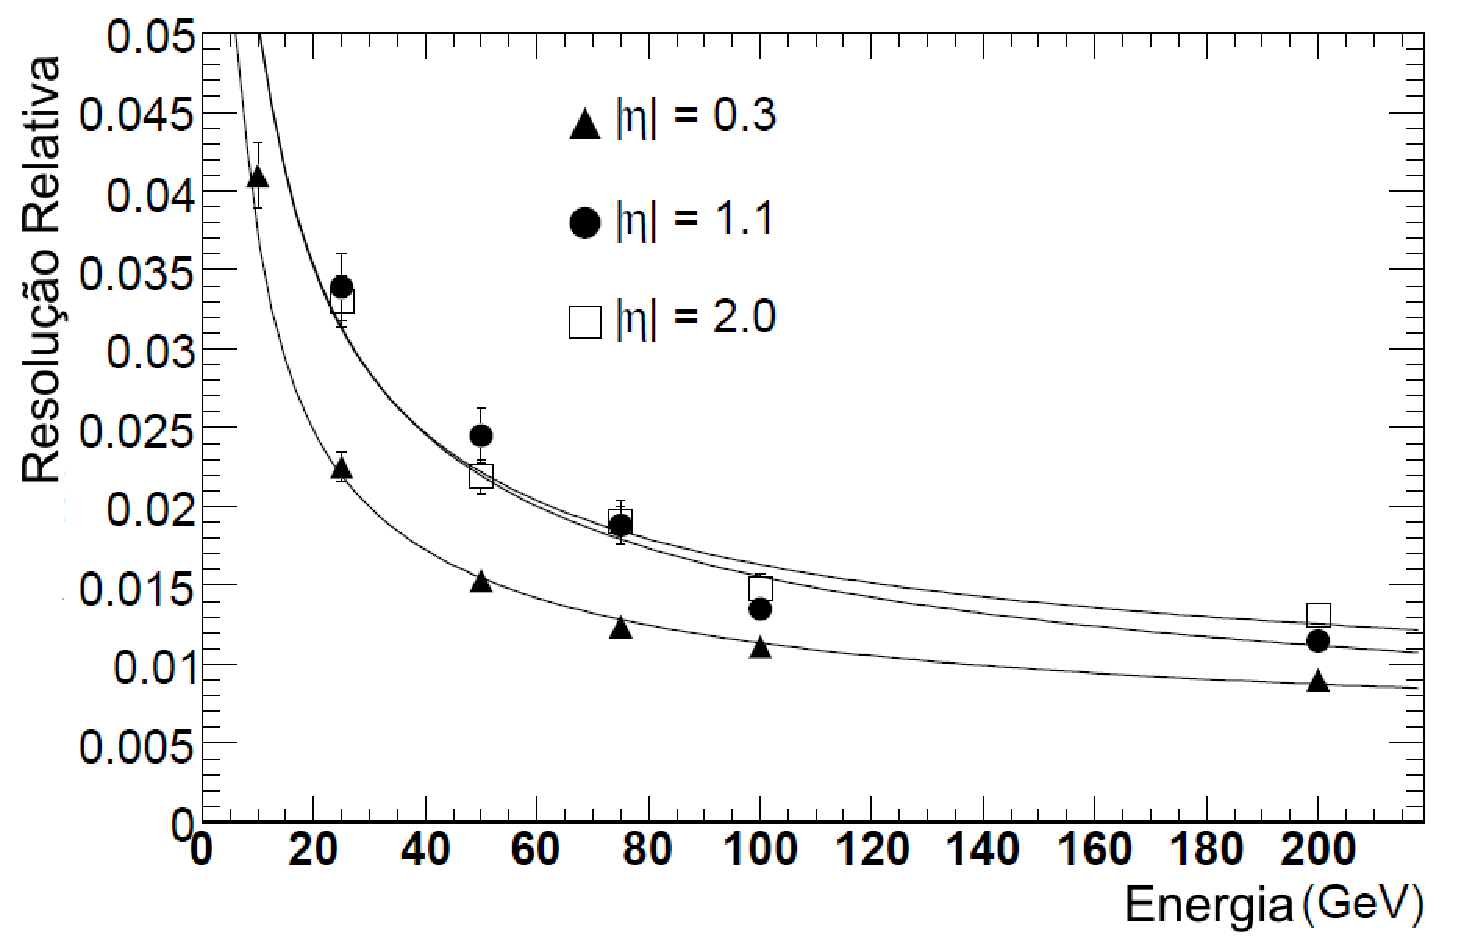
\epsfig{file=cap3_enres,width=8cm}}
 \vspace{.3cm}
  \centerline{(a)}\medskip
\end{minipage}
\hfill
\begin{minipage}[b]{.48\linewidth}
  \centering
 \centerline{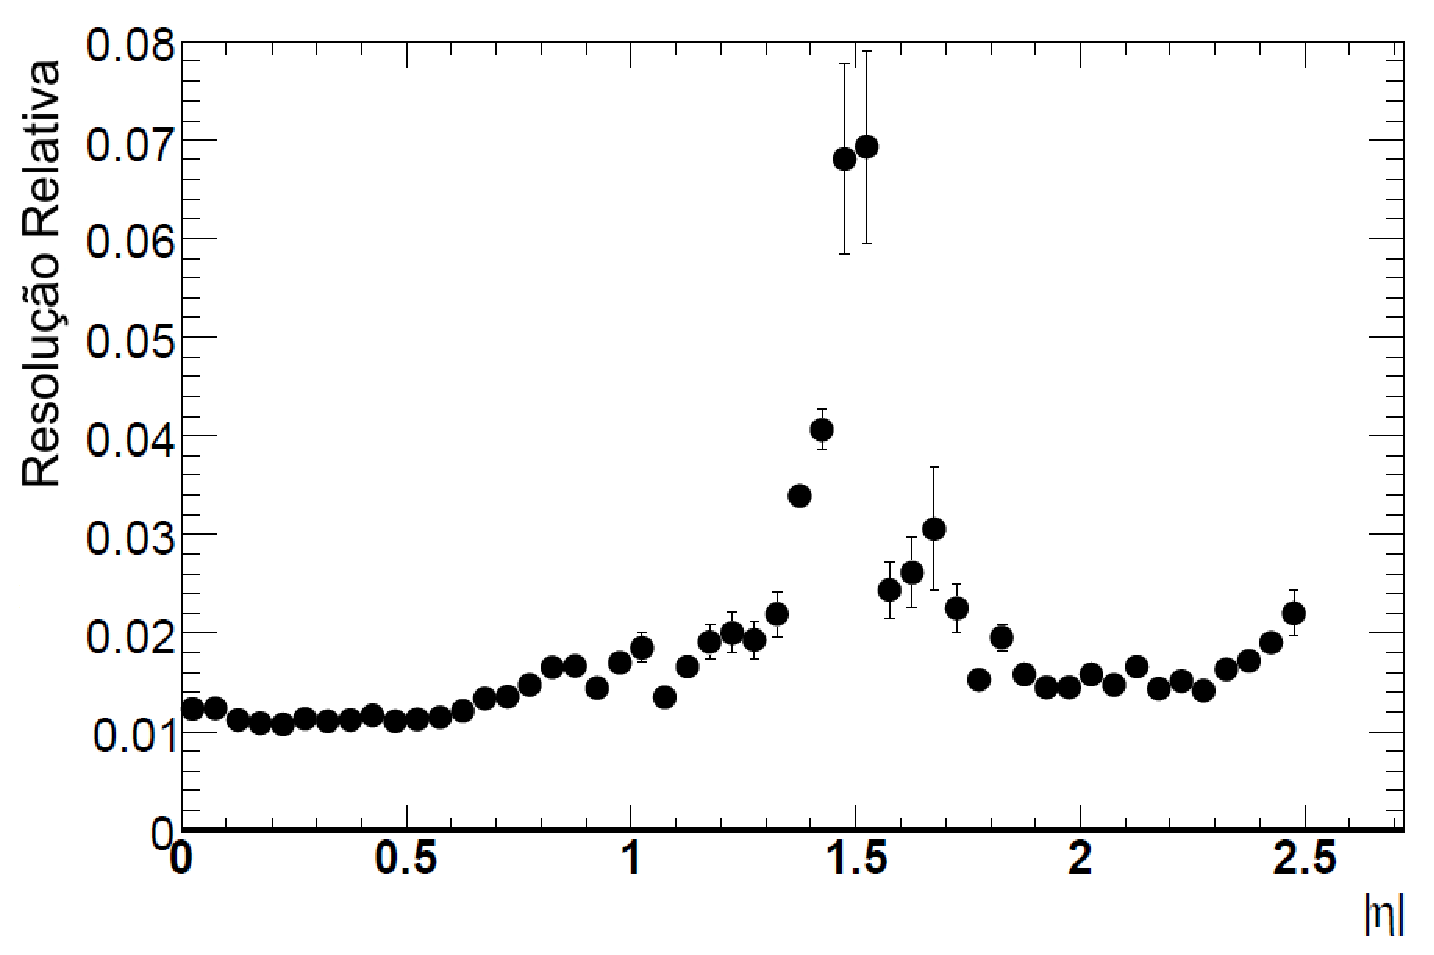
\epsfig{file=cap3_etares,width=8cm}}
 \vspace{.3cm}
  \centerline{(b)}\medskip
 \end{minipage}
\caption[Erro relativo do calor�metro na medi��o da energia de el�trons para diferentes valores de (a) energia e (b)~$\eta$.]{Erro relativo do calor�metro na medi��o da energia de el�trons para diferentes valores de (a) energia e (b)~$\eta$, adaptado de~\cite{article:ATLAS:2008}.} \label{cap3_enres}
\end{figure}

Um outro fator que pode provocar medi��o incorreta nos calor�metros � o vazamento de energia de el�trons al�m da 
terceira camada eletromagn�tica. O calor�metro eletromagn�tico foi projetado para conter todo o chuveiro 
eletromagn�tico, por�m, eventos que insidem na regi�o do crack, por encontrarem menor quantidade de material para 
interagirem, podem alcan�ar o calor�metro hadr�nico. Conforme ilustrado na Figura \ref{fig_envazahad}, a energia de 
el�trons � quase totalmente concentrada no calor�metro eletromagn�tico, por�m, quando a part�cula interage pr�ximo 
ao \textit{crack}, uma parcela significativa de energia chega ao calor�metro hadr�nico. 
Essa limita��o pode provocar problemas para o sistema de filtragem, como ser� descrito a seguir.

\begin{figure} \centering
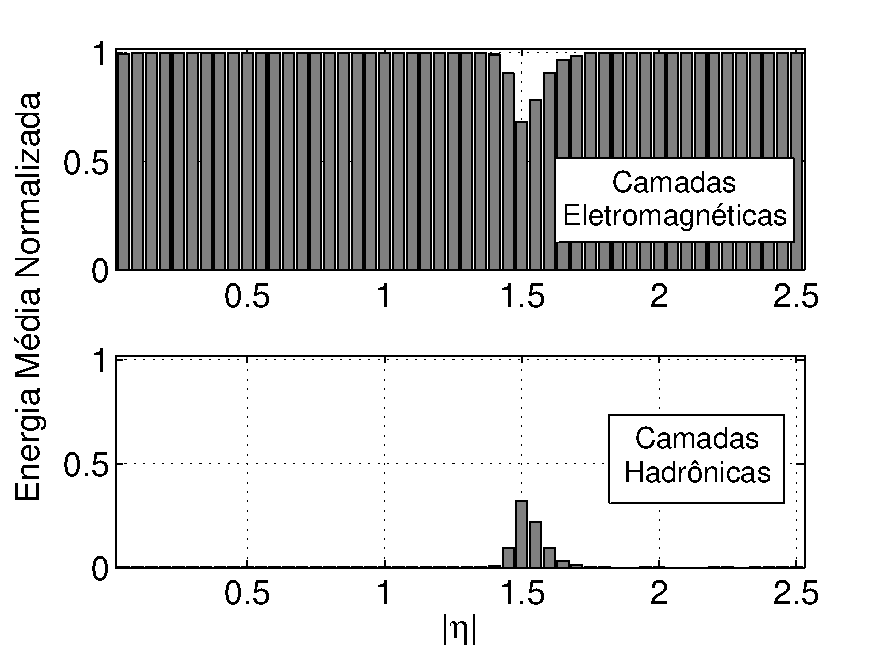
\includegraphics[width=9cm]{capt_ensec}
\caption{Energia normalizada m�dia depositada nas sec��es eletromagn�tica e hadr�nica em fun��o de $\eta$ para el�trons.} \label{fig_envazahad}
\end{figure}


\section{Filtragem de el�trons no L1}

O primeiro n�vel de filtragem opera com granularidade reduzida para tornar mais r�pido o processo de decis�o. Ent�o, 
no L1, as c�lulas dos calor�metros s�o somadas para formar sinais conhecidos
como torres de \textit{trigger} (TT). O tamanho das torres de \textit{trigger} �
diferente para as camadas eletromagn�ticas e hadr�nicas. No calor�metro eletromagn�tico, cada TT cobre uma �rea de 0,1
$\times$ 0,1 no plano $\eta \times \phi$, j� no calor�metro
hadr�nico, cada TT representa uma regi�o de 0,2 $\times$ 0,2 no plano $\eta \times \phi$. 

A filtragem de el�trons no L1 � baseada em cortes lineares nos
par�metros do perfil de deposi��o de energia medido nos
calor�metros. A defini��o dos crit�rios de sele��o leva em conta o
conhecimento das caracter�sticas t�picas do perfil de deposi��o de
energia de objetos eletromagn�ticos (el�trons e f�tons), que
geralmente apresentam:
\begin{itemize}
  \item concentra��o ao redor do ponto de colis�o (centro da RoI);
  \item alta concentra��o de energia na se��o eletromagn�tica;
  \item baixa concentra��o de energia na se��o hadr�nica.
\end{itemize}

A partir da an�lise
de uma janela deslizante, cobrindo uma regi�o de 4 $\times$ 4 TT (16
no total), alguns crit�rios podem ser utilizados pelo L1 para
definir um poss�vel candidato a el�tron:
\begin{enumerate}
  \item Os valores de energia das TTs da regi�o central (de 2 $\times$ 2 TT)
  s�o somados dois a dois e utiliza-se o maior valor encontrado, que deve exceder um patamar de energia 
eletromagn�tica;
  \item O n�vel de energia na periferia (fora da regi�o central de 2 $\times$ 2
  TT) � calculado para verificar o isolamento em energia do objeto
  em quest�o;
  \item A energia depositada nas camadas hadr�nicas � somada para verificar o
  vazamento de energia fora do calor�metro eletromagn�tico (isolamento hadr�nico).
\end{enumerate}
Os patamares de sele��o do n�vel 1 podem ser ajustados e os
crit�rios combinados, a depender das caracter�sticas da f�sica de
interesse que se deseja estudar num dado momento de opera��o do
detector. O sistema de filtragem do L1 � implementado utilizando hardware dedicado (atrav�s de FPGAs) conforme 
detalhado em \cite{artigo:L1:implem}.

\begin{figure} \centering
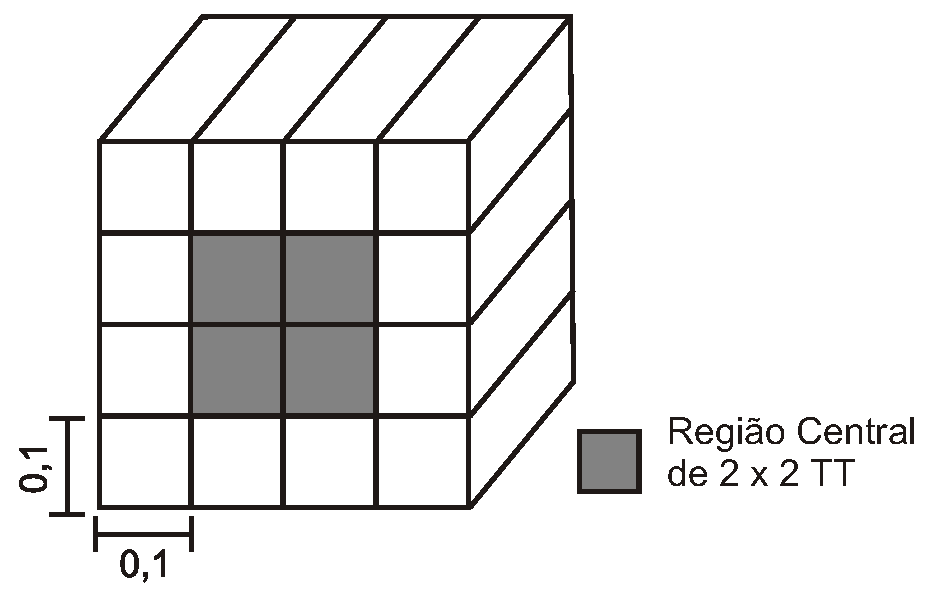
\includegraphics[width=9cm]{cap2_trigger_tower}
\caption{Janela deslizante analisada pelo L1 no calor�metro
eletromagn�tico.} \label{lvl1tt}
\end{figure}


\section{Filtragem de el�trons no L2 - Algoritmo T2Calo}

\begin{figure} \centering
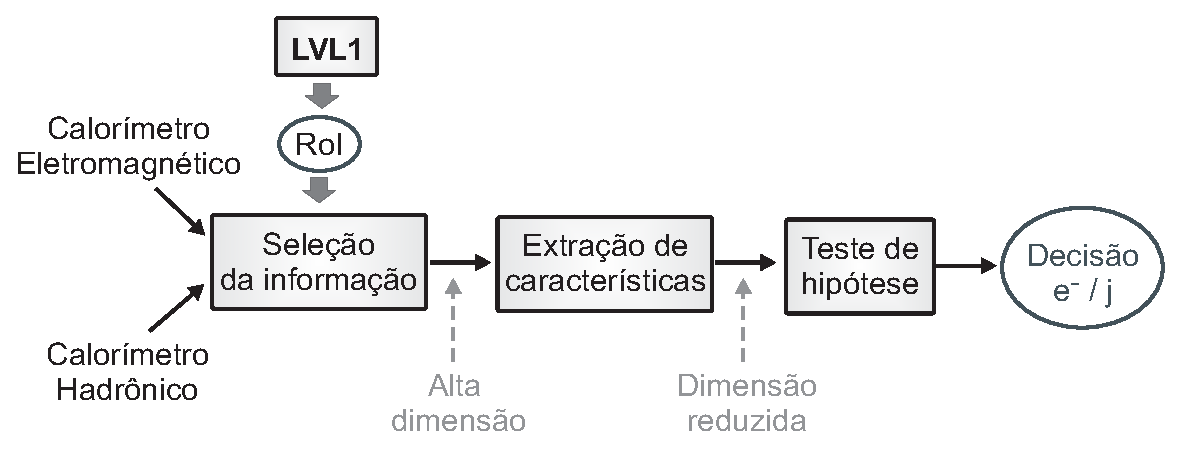
\includegraphics[width=13cm]{cap1_esquema}
\caption{Processo de identifica��o de el�trons no L2.} \label{fig_esqL2}
\end{figure}

O processo de discrimina��o de el�trons no segundo-n�vel de filtragem \textit{online} do ATLAS, conforme ilustrado 
na Figura \ref{fig_esqL2}, pode ser dividido em duas etapas distintas, extra��o de caracter�sticas (onde 
par�metros discriminantes s�o estimados a partir dos dados brutos medidos nos calor�metros) e teste de hip�teses 
(a discrimina��o propriamente dita � realizada a partir das caracter�sticas estimadas).

O \textbf{T2Calo} \cite{TDR:ATLAS:2003} � o algoritmo padr�o para
extra��o de caracter�sticas e teste de hip�teses adotado no
segundo n�vel de filtragem do ATLAS. Esse algoritmo utiliza
informa��es de calorimetria, sendo capaz de separar objetos
eletromagn�ticos isolados de jatos hadr�\-nicos, utilizando
par�metros que estimam a forma dos chuveiros de deposi��o de
energia \cite{TDR:ATLAS:2003}. O T2Calo opera de modo semelhante ao algoritmo de filtragem do L1, por�m 
agora, ao inv�s de usar as torres de \textit{trigger}, toda a granularidade dos calor�metros est� dispon�vel.

O primeiro passo do T2Calo � refinar a posi��o do centro da RoI fornecida pelo
L1, encontrando a c�lula de maior energia na segunda camada do
calor�metro eletromagn�tico ($\eta_1 , \phi_1$). Essa posi��o ser�
posteriormente refinada pelo c�lculo da posi��o da m�dia ponderada
da energia em uma janela de $3 \times 7$ em ($\eta , \phi$). 

Para a sele��o dos objetos eletromagn�ticos, o T2Calo estima os par�metros descritos a seguir:
\begin{itemize}
  \item Raz�o de Forma: $R_{shape}=E_{3 \times 7}/E_{7 \times 7}$, onde $E_{n \times m}$ � a energia
  depositada numa janela de $n \times m$ c�lulas em torno de ($\eta_1 ,
  \phi_1$) na segunda camada eletromagn�tica;

  \item Raz�o de Energia: $E_{ratio}=(E_{1st}-E_{2nd})/(E_{1st}+E_{2nd})$, onde $E_{1st}$ e $E_{2nd}$ s�o o m�ximo e o 
segundo maior valor de energia encontrados na primeira camada eletromagn�tica numa janela de 
$\Delta \eta \times \Delta \phi=0,125 \times 0,2$ em torno do centro da RoI;

  \item A energia eletromagn�tica total: $E_{EM}$ � calculada a partir da soma 
da energia concentrada em janelas de $3 \times 7$ c�lulas
  em torno de ($\eta_1 ,\phi_1$) nas tr�s camadas eletromagn�ticas;

  \item A energia hadr�nica total: $E_{HAD}$ �
  calculada a partir da soma da energia concentrada em janelas de $\Delta \eta \times \Delta \phi=0,2 \times
  0,2$ em torno do centro da RoI nas tr�s camadas hadr�nicas.

\end{itemize}

Considerando que o perfil de deposi��o de energia dos el�trons �,
em geral, mais concentrado ao redor do ponto de m�ximo e que,
tamb�m n�o espera-se deposi��o de uma quantidade significativa de
energia nas camadas hadr�nicas por el�trons, o
T2Calo opera atrav�s de cortes lineares nos par�metros estimados acima. Por exemplo, analisando os par�metros
$R_{shape}$, $E_{ratio}$ e $E_{EM}$, os eventos s�o aprovados caso os valores calculados sejam maiores que um 
patamar de corte pr�-estabelecido. Para $E_{HAD}$, acontece o inverso, e um candidato a el�tron � selecionado 
se o valor calculado para este par�metro for menor que o patamar.

Embora a concentra��o em torno do centro da RoI e o vazamento hadr�nico 
sejam caracter�sticas bastante �teis na identifica��o de el�trons, uma an�lise um pouco 
mais detalhada revela que, pelo fato dos jatos apresentarem uma grande flutua��o em suas caracter�sticas, o uso apenas destes 
par�metros pode n�o produzir o desempenho de discrimina��o desejado. Na Figura \ref{cap3_anwigmans}, 
considerando a raz�o $\frac{E_{HAD}}{E_{EM}}$ (num conjunto de eventos simulados para o L2 do ATLAS), percebe-se que h� 
uma razo�vel superposi��o entre el�trons e jatos, essa limita��o aumenta em baixa energia. Comportamento 
semelhante � verificado na Figura \ref{cap3_anperfil} onde el�trons e jatos s�o comparados a partir 
da raz�o $\frac{E_{3 \times 7}}{E_{7 \times 7}}$.

\begin{figure}[h!]
\begin{minipage}[b]{.48\linewidth}
  \centering
 \centerline{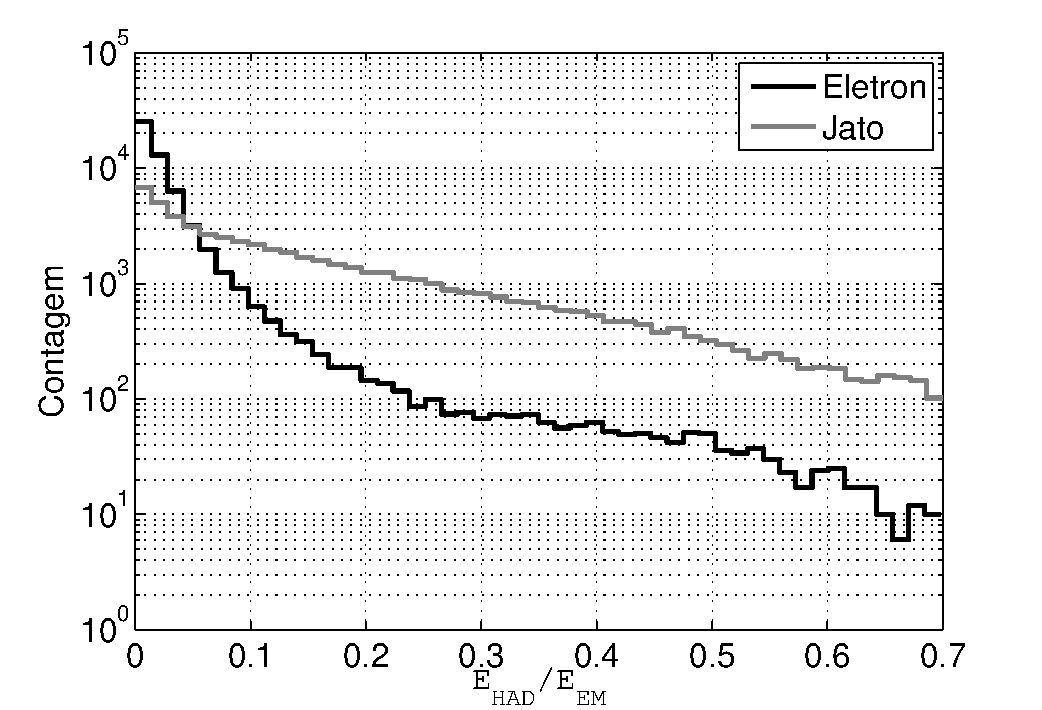
\epsfig{file=cap3_Ehad_em20,width=8cm}}
 \vspace{.3cm}
  \centerline{(a)}\medskip
\end{minipage}
\hfill
\begin{minipage}[b]{.48\linewidth}
  \centering
 \centerline{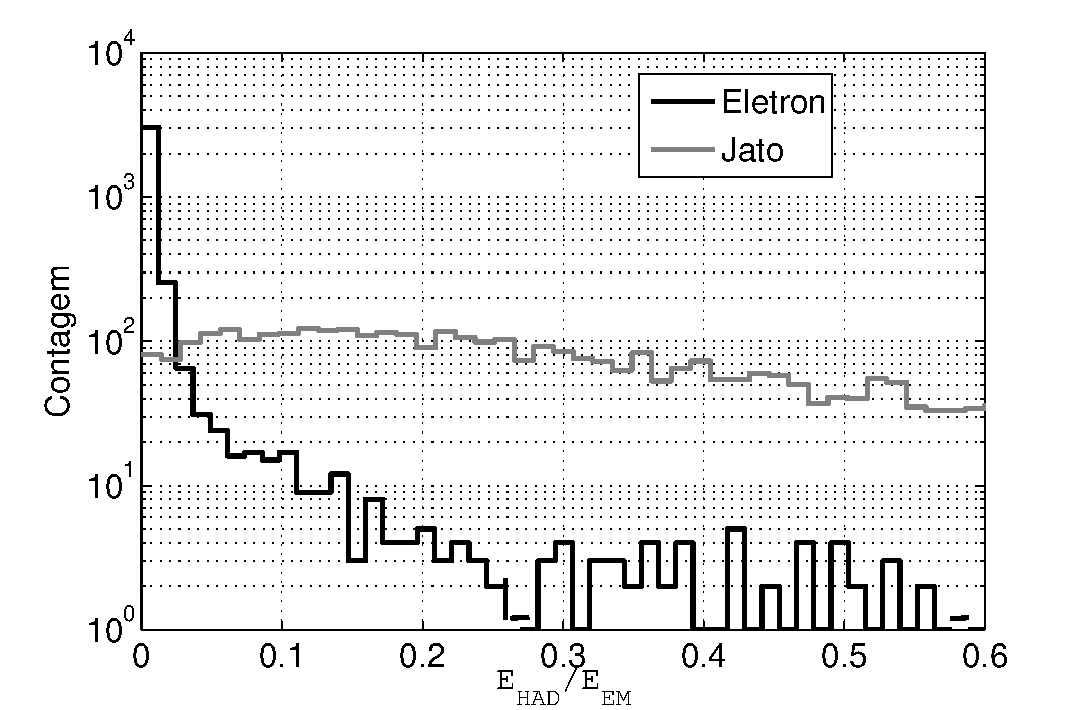
\epsfig{file=cap3_Ehad_em60,width=8cm}}
 \vspace{.3cm}
  \centerline{(b)}\medskip
 \end{minipage}
\caption{Distribui��o de el�trons e jatos quanto � raz�o $\frac{E_{HAD}}{E_{EM}}$ para eventos com energia total (a) menor que 20 GeV e (b) maior que 60 GeV.} \label{cap3_anwigmans}
\end{figure}

\begin{figure}[h!]
\begin{minipage}[b]{.48\linewidth}
  \centering
 \centerline{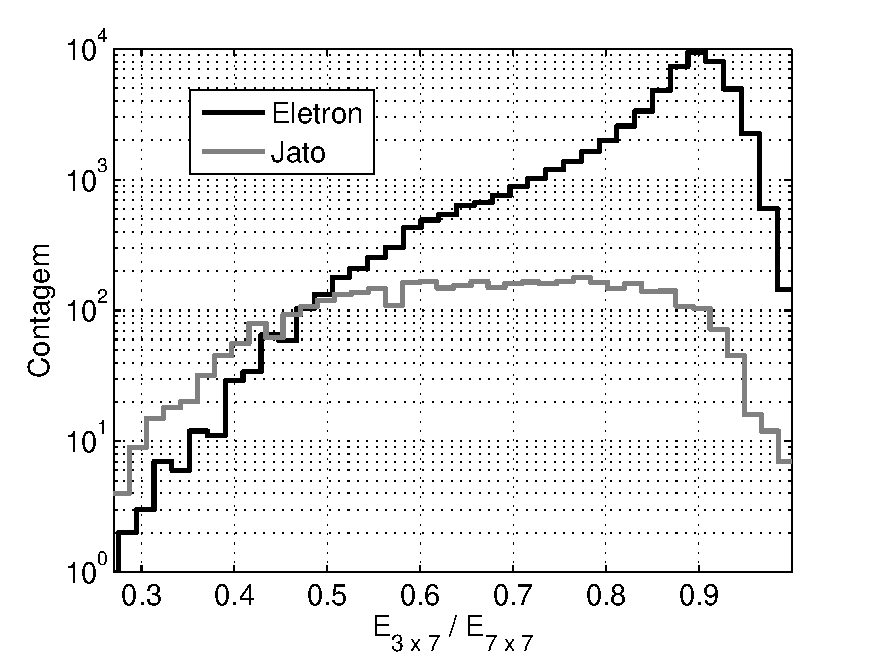
\epsfig{file=cap3_E3E720,width=8cm}}
 \vspace{.3cm}
  \centerline{(a)}\medskip
\end{minipage}
\hfill
\begin{minipage}[b]{.48\linewidth}
  \centering
 \centerline{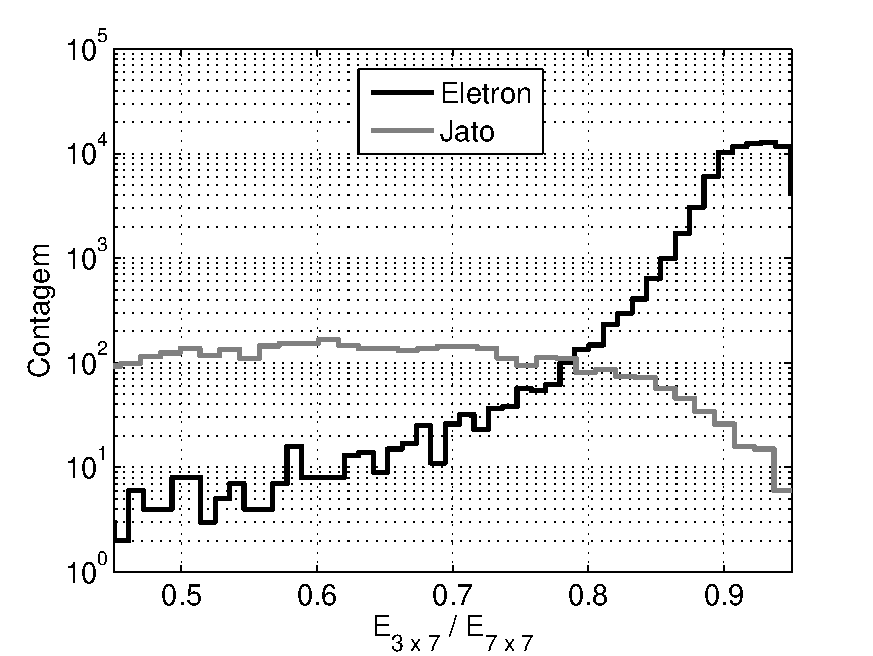
\epsfig{file=cap3_E3E760,width=8cm}}
 \vspace{.3cm}
  \centerline{(b)}\medskip
 \end{minipage}
\caption{Distribui��o de el�trons e jatos quanto � raz�o$\frac{E_{3 \times 7}}{E_{7 \times 7}}$ para eventos com energia total (a) menor que 20 GeV e (b) maior que 60 GeV.} \label{cap3_anperfil}
\end{figure}

Num ambiente complexo, como o que � gerado a cada colis�o do LHC,
onde o n�vel de ru�do de fundo � extremamente alto e os eventos de
interesse s�o raros, a busca por algoritmos de filtragem mais eficientes � muito importante. 
Aumentar o desempenho de discrimina��o significa menor quantidade de eventos n�o relevantes
armazenados m�dia permanente, economizando recursos e facilitando a an�lise
\textit{offline}.

A seguir, ser�o descritos discriminadores alternativos, propostos para o canal el�tron/jato no L2 do ATLAS, que 
fazem uso da f�sica de interesse em conjunto com o processamento estat�stico de sinais. Combinando 
a isso a aplica��o de classificadores neurais, que s�o
capazes de produzir cortes n�o-lineares no espa�o de busca, possibilitou elevada efici�ncia de discrimina��o
se comparado ao T2Calo.


\section{Neural Ringer - Alternativa para Filtragem de El�trons no L2}
\label{sec_ringer}
Um discriminador alternativo foi proposto inicialmente em~\cite{article:seixas:1996} para o canal 
el�tron/jato no segundo n�vel de filtragem do ATLAS. Conforme ilustrado na Figura~\ref{fig_ringerdiag}, 
o processo de extra��o de caracter�sticas compreende um arranjo topol�gico dos sinais medidos no calor�metro 
(com a constru��o de an�is a partir do perfil de deposi��o de energia), e o teste de hip�teses � realizado 
por um classificador neural supervisionado (arquitetura Perceptron de M�ltiplas Camadas)~\cite{haykin:nn:2008}, 
este discriminador ficou conhecido como \textit{Neural Ringer}.

\begin{figure}[b] 
\centering
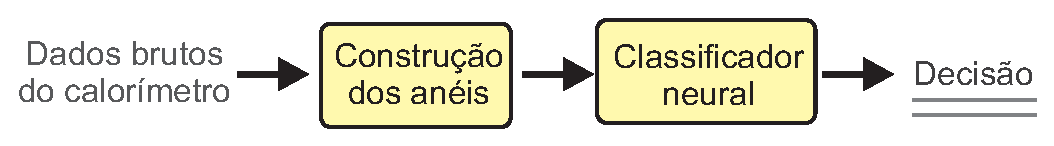
\includegraphics[width=11cm]{cap3_ringerdiag}
\caption{Fluxo de processamento do \textit{Neural Ringer}.} \label{fig_ringerdiag}
\end{figure}

\subsection{Extra��o de Caracter�sticas - Anelamento}

Os sinais do perfil de deposi��o de energia utilizados para
discrimina��o el�tron/jato s�o medidos nas sete camadas dos
calor�metros do ATLAS. Considerando a granularidade de cada camada,
uma Regi�o de Interesse (RoI) t�pica (de tamanho 0,4$ \times 0,4$ em
$\eta \times \phi$) � descrita por aproximadamente 1000 c�lulas~\cite{tese:andre:2006}. Visando compactar
os sinais dos calor�metros e, ao mesmo tempo, manter a interpreta��o f�sica do perfil
de deposi��o de energia, as c�lulas sensoras de cada camada s�o agrupadas em an�is conc�ntricos de 
deposi��o de energia.

Considerando um conjunto de c�lulas de uma RoI em uma certa camada
do calor�metro, conforme ilustrado na Figura~\ref{fig_aneis}, a
c�lula mais energ�tica de cada camada � considerada como o primeiro
anel. Em seguida, as c�lulas ao redor do primeiro anel (imediatamente adjacentes) definem o
segundo anel e assim sucessivamente. A energia amostrada pelas
c�lulas pertencentes a um dado anel s�o somadas produzindo o sinal
de energia em an�is. � interessante notar que, devido � diferen�a de
granularidade entre as camadas do calor�metro, um n�mero diferente
de an�is � gerado para cada camada. A Tabela \ref{tab_aneis} mostra
a distribui��o dos an�is por camada. No processo de formata��o � considerado um n�mero 
fixo de an�is por camada, por�m, dependendo da posi��o do centro da RoI, esta pode 
n�o estar completa (as c�lulas sensoras que comp�em os an�is podem n�o existir caso a 
part�cula interaja pr�ximo a uma extremidade ou descontinuidade do calor�metro), neste caso, 
assume-se igual a zero as leituras das c�lulas que faltam. Outra caracter�stica a ser observada 
� que, em algumas camadas, as c�lulas n�o s�o quadradas (conforme ilustrado na Figura \ref{fig_ancam}),
 neste caso, falar em an�is � uma abstra��o 
(pois ao final do processo descrito acima podem n�o existir realmente an�is de c�lulas sensoras). 
A Figura \ref{fig_sig3d} mostra os sinais medidos na segunda camada eletromagn�tica do calor�metro,
respectivamente, para um el�tron e um jato e os sinais dos an�is gerados.

\begin{figure}[th]
\centering
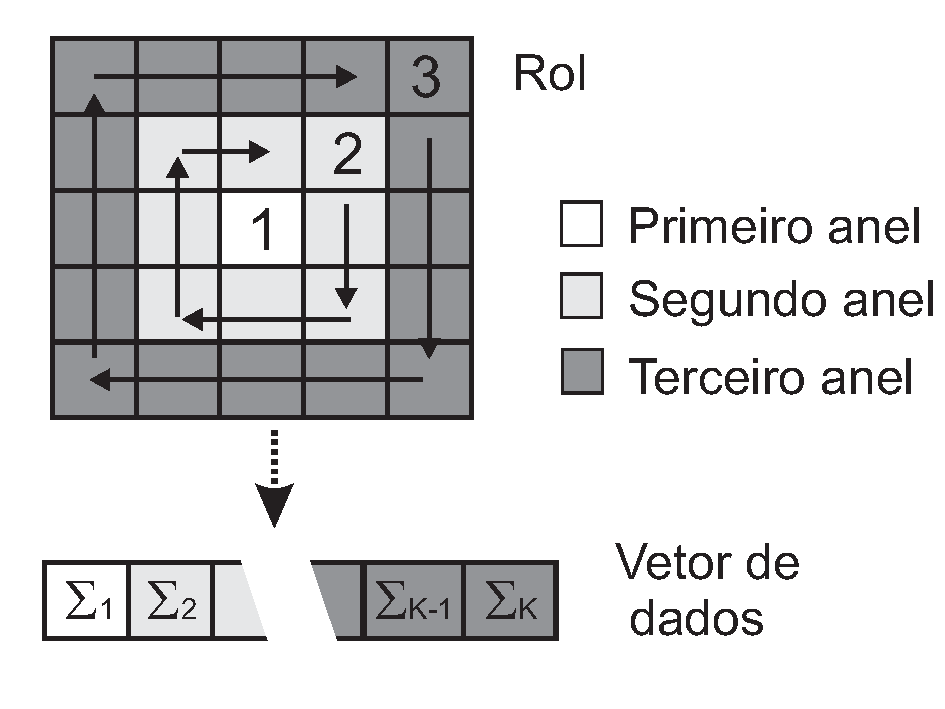
\includegraphics[width=6.5cm]{cap3_aneis}
\caption{Diagrama do processo de constru��o dos an�is.}
\label{fig_aneis}
\end{figure}

\begin{table}[th]
\centering \caption{N�mero de an�is formados para cada camada do calor�metro do ATLAS.}\vspace{0.2cm} \footnotesize
\begin{tabular}{c | c c c c c c c | c}
    \hline
     \textbf{Camada} & \textbf{PS} & \textbf{E1} & \textbf{E2} & \textbf{E3} & \textbf{H0} & \textbf{H1} & \textbf{H0} & \textbf{Total} \\
\hline
    \textbf{An�is} & 8 & 64 & 8 & 8 & 4 & 4 & 4 & 100 \\
\hline
\end{tabular}
\label{tab_aneis}
\end{table}

\begin{figure}[th]
\centering
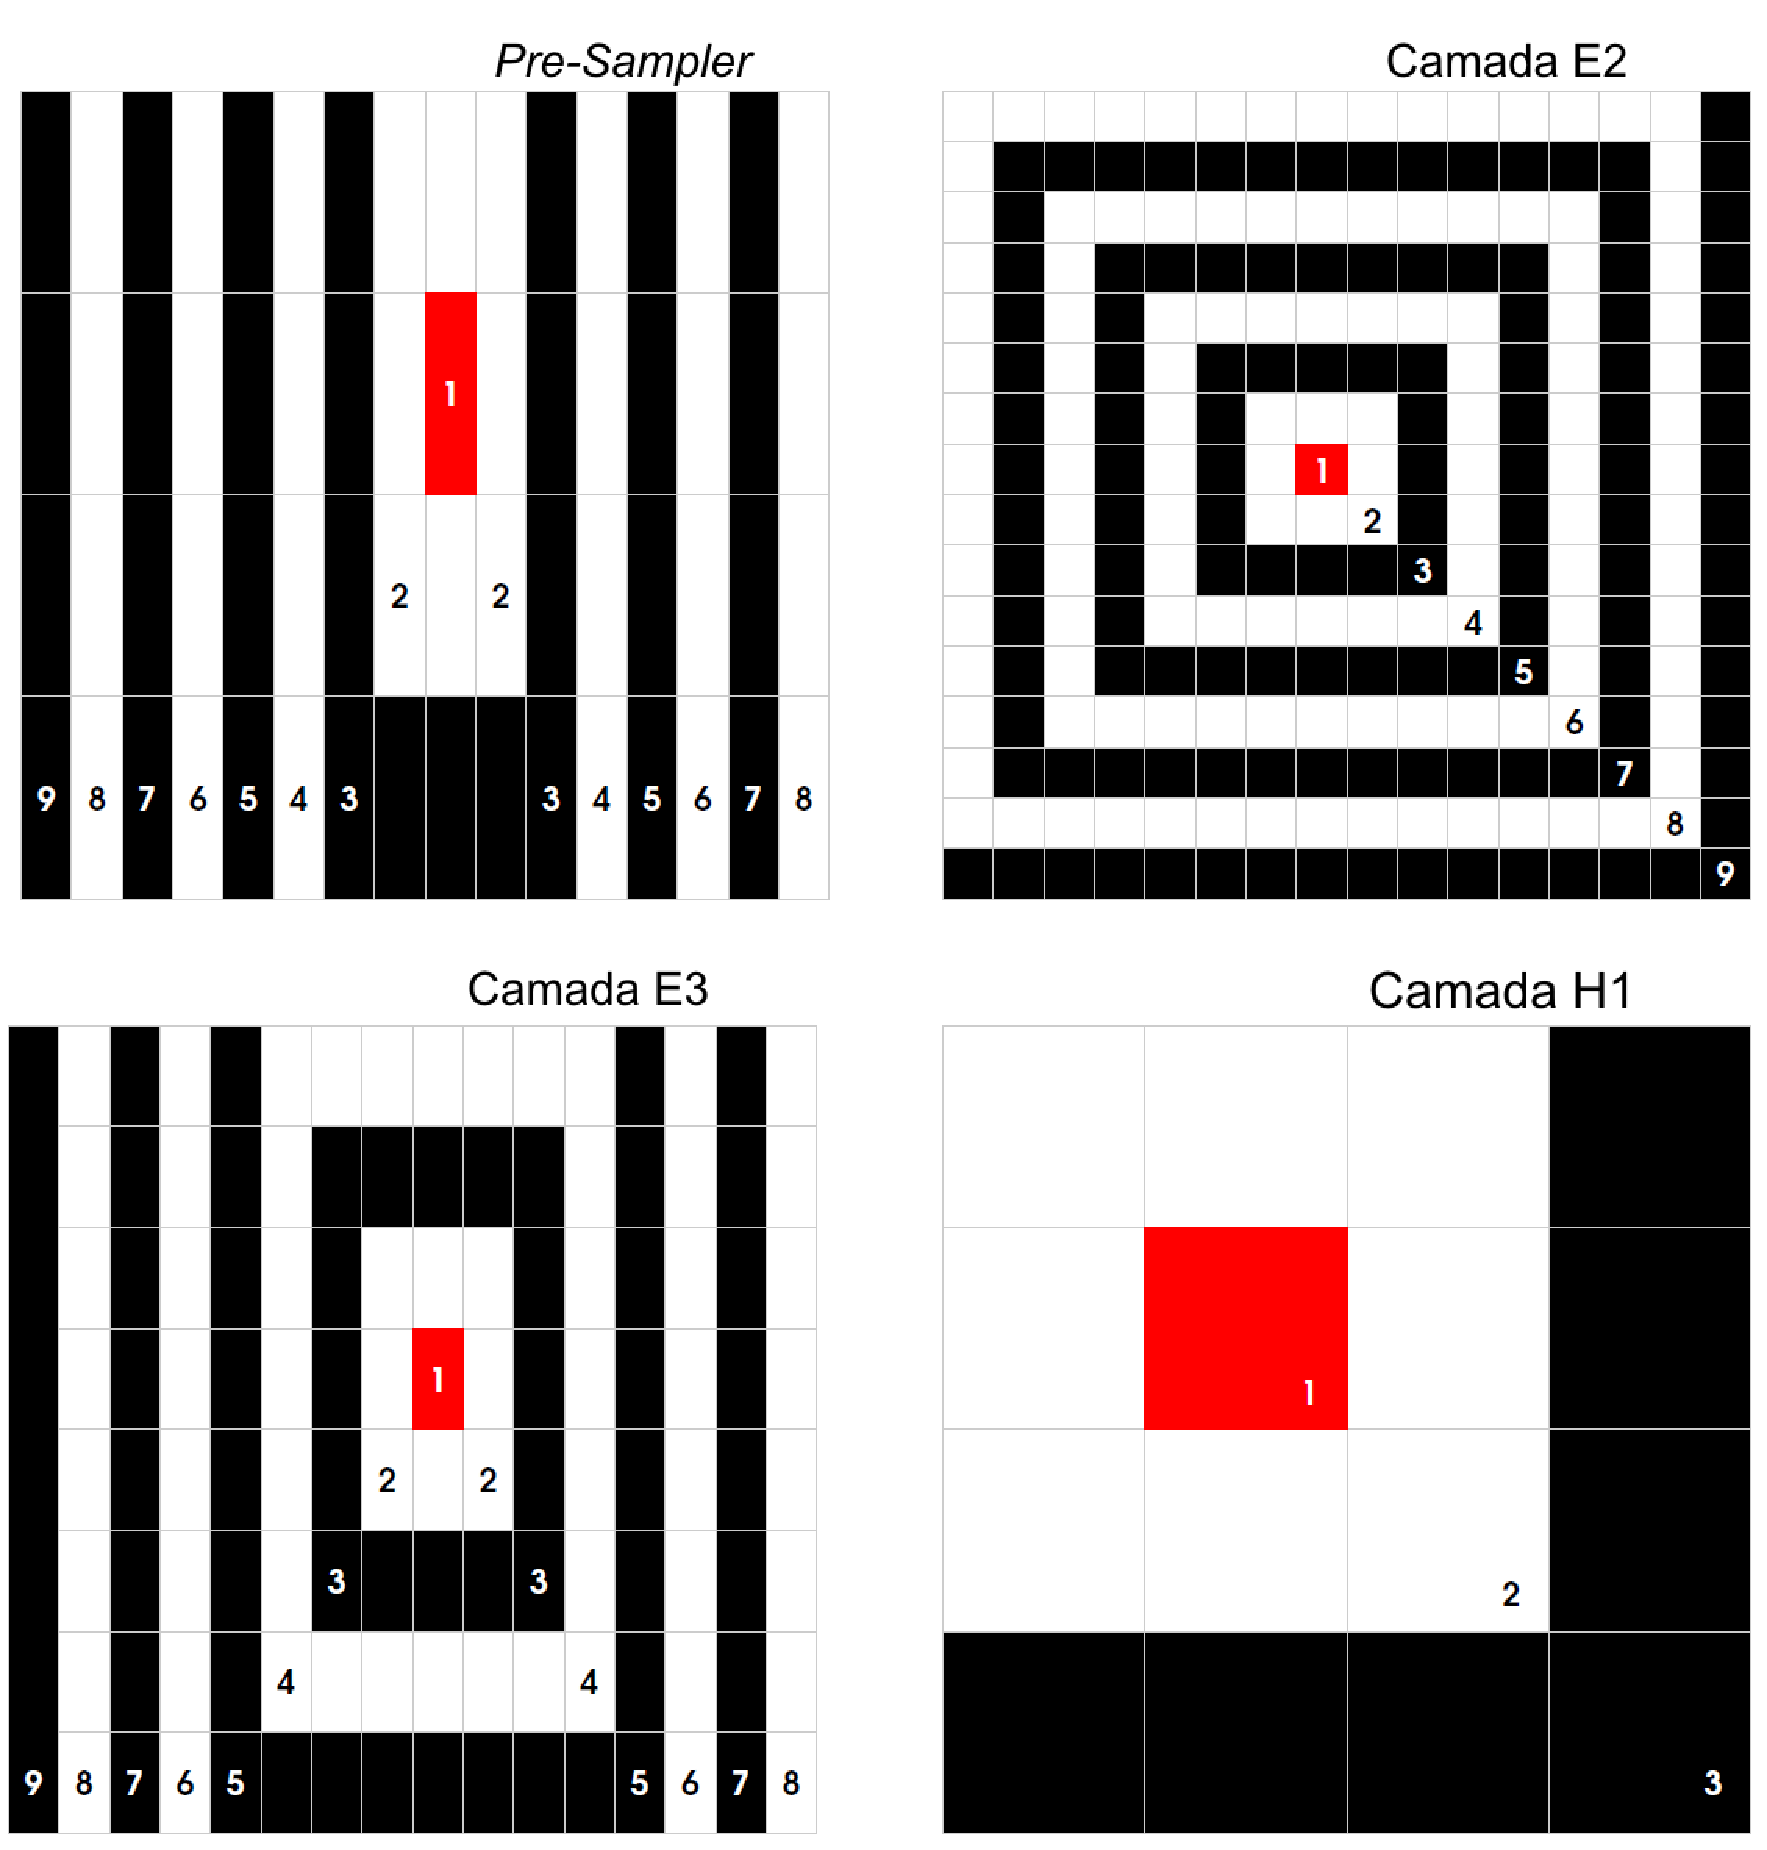
\includegraphics[width=14cm]{cap3_rescalo}
\caption{Diagrama do processo de constru��o dos an�is.}
\label{fig_aneis}
\end{figure}

\begin{figure}[h!]
\begin{minipage}[b]{.48\linewidth}
  \centering
 \centerline{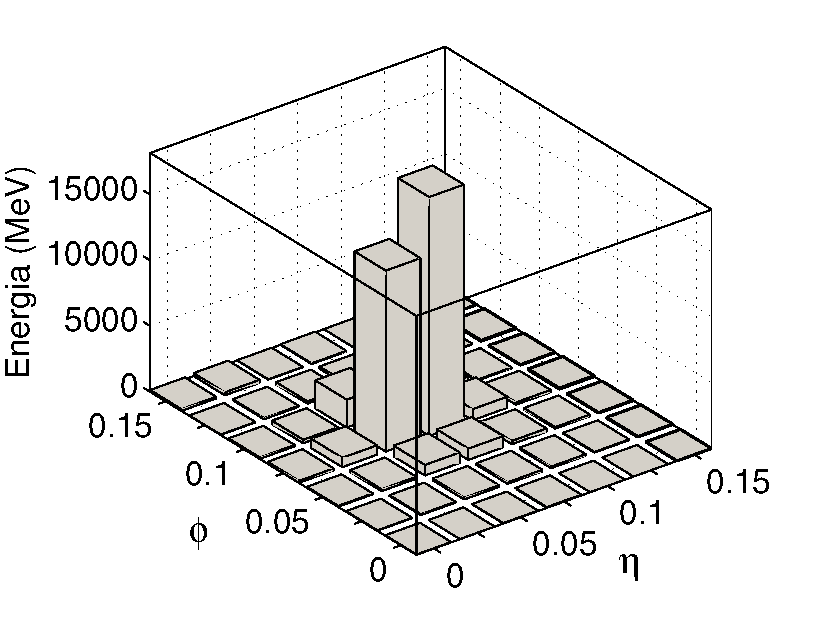
\epsfig{file=cap3_ele_e2_3d,width=7.5cm}}
  \vspace{.3cm}
  \centerline{(a)}\medskip
\end{minipage}
\hfill
\begin{minipage}[b]{0.48\linewidth}
  \centering
 \centerline{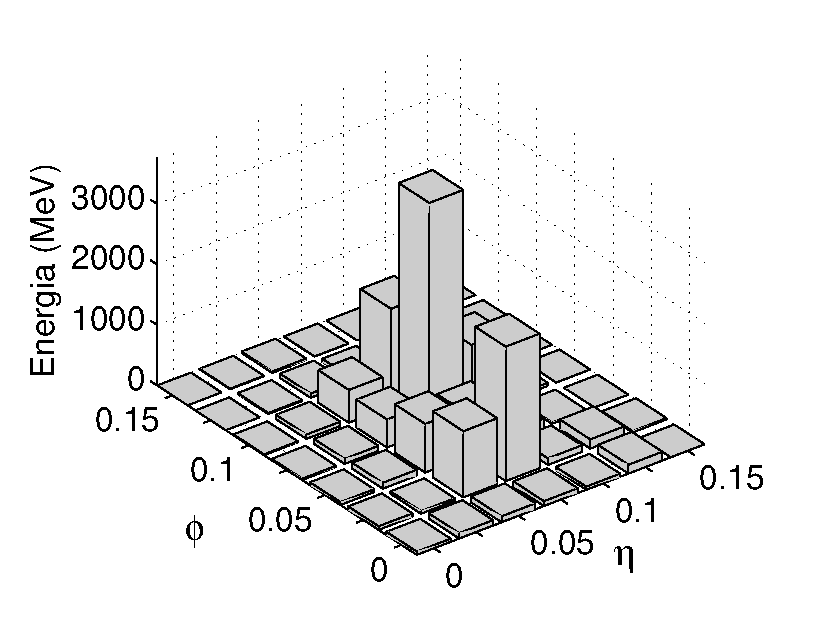
\epsfig{file=cap3_jet_e2_3d,width=7.5cm}}
  \vspace{.3cm}
  \centerline{(b)}\medskip
\end{minipage}
\hfill \linebreak \caption{Sinais t�picos medidos na camada EM2 para (a)
el�tron e (b) jato.} \label{fig_sig3d}
\end{figure}

A Figura \ref{fig_sig_anel} mostra sinais em an�is, respectivamente, para um el�tron t�pico, um jato t�pico e 
um jato com perfil semelhante ao de el�trons. Percebe-se que o perfil de deposi��o medido para el�trons 
apresenta pouco espalhamento (� contido em uma pequena regi�o) e � concentrado nas camadas eletromagn�ticas. 
Os jatos apresentam uma maior varia��o em suas caracter�sticas f�sicas. Essas part�culas tipicamente 
depositam uma consider�vel quantidade de energia nas camadas hadr�nicas e possuem perfil de deposi��o com 
pouca concentra��o espacial (ver Figura \ref{fig_sig_anel}-b). Entretanto, alguns jatos (como o mostrado na 
Figura \ref{fig_sig_anel}-c) podem apresentar perfil de deposi��o de energia semelhante ao de el�trons. 
Esse �ltimo tipo de assinatura hadr�nica representa a maioria dos jatos aprovados como el�trons pelo L1, 
compondo um ru�do de fundo de dif�cil identifica��o. 

%\begin{figure}[th]
%\begin{center}
%\subfigure[]{\label{fig_calo_ele}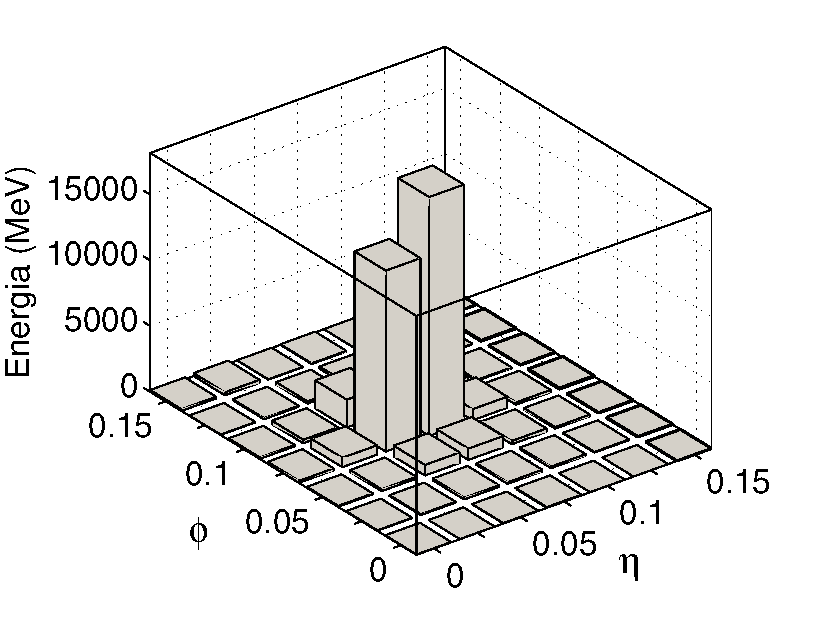
\epsfig{file=cap3_ele_e2_3d,width=7.5cm,clip=}}
%\subfigure[]{\label{fig_calo_jet}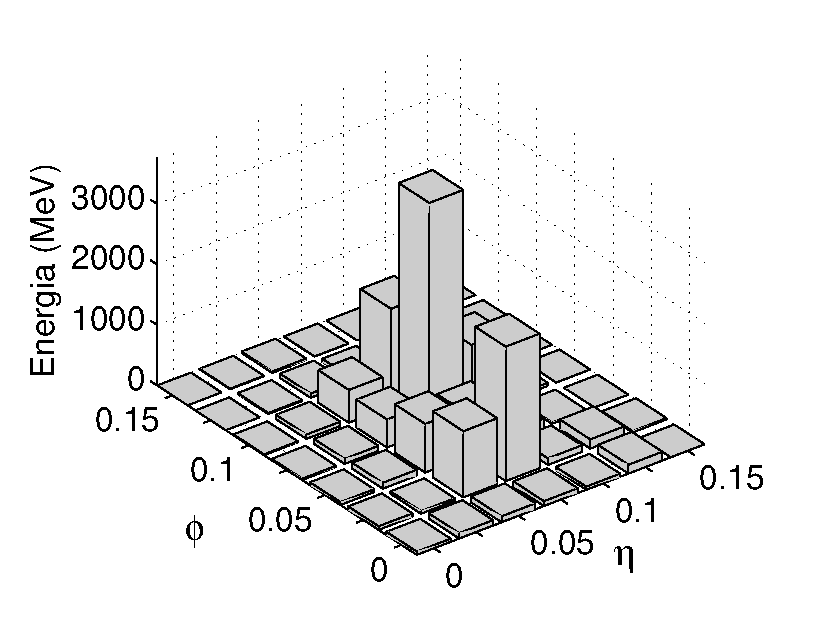
\epsfig{file=cap3_jet_e2_3d,width=7.5cm,clip=}}
%\end{center}
%\caption{Sinais medidos na camada EM2 para (a) el�tron e (b) jato.}
%\end{figure}


\begin{figure}[h!]
\begin{minipage}[b]{0.48\linewidth}
  \centering
 \centerline{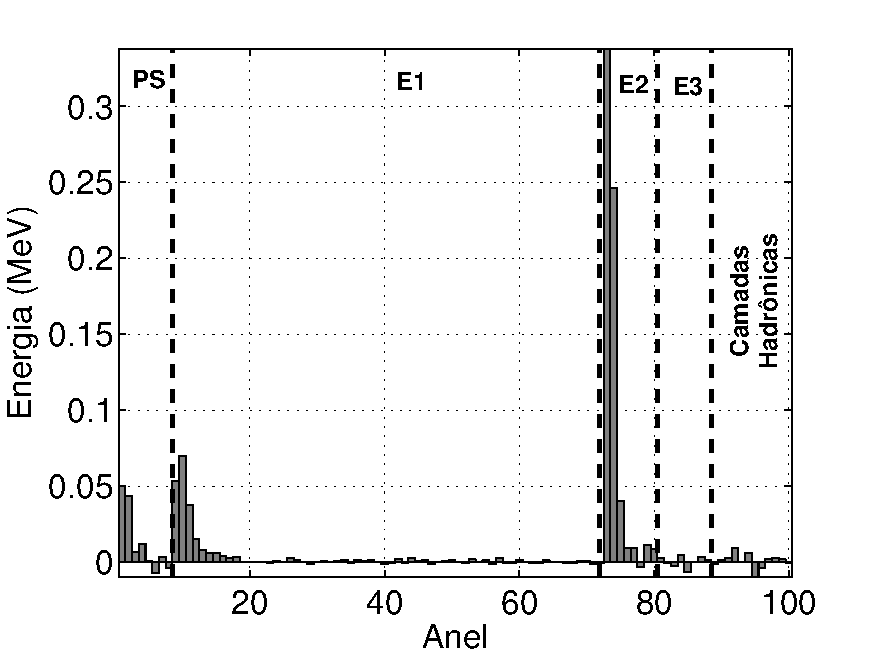
\epsfig{file=cap3_ele_tip,width=7.5cm}}
  \vspace{.3cm}
  \centerline{(a)}\medskip
\end{minipage}
\hfill
\begin{minipage}[b]{0.48\linewidth}
  \centering
 \centerline{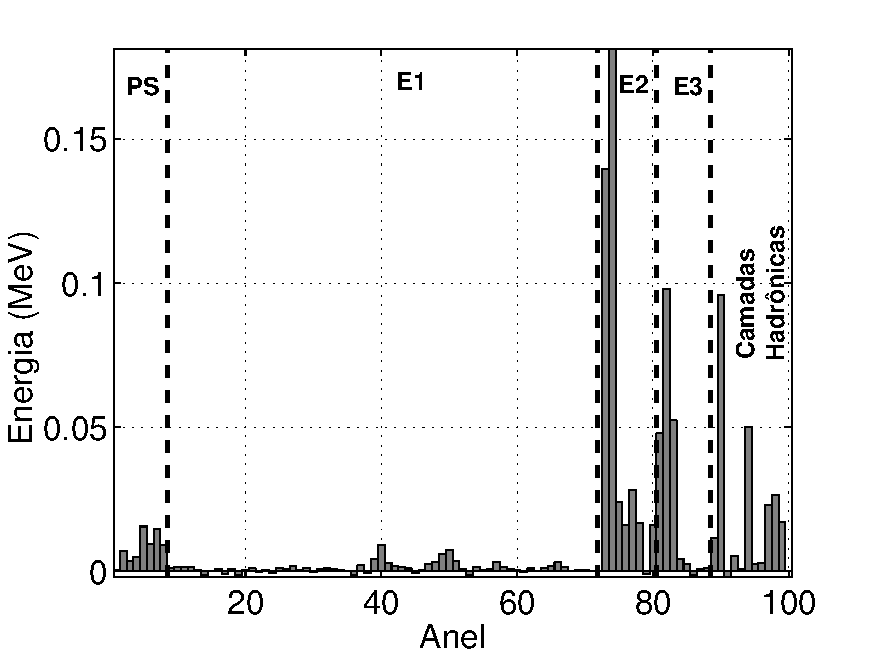
\epsfig{file=cap3_jet_tip,width=7.5cm}}
  \vspace{.3cm}
  \centerline{(b)}\medskip
\end{minipage}
\hfill \linebreak
\begin{minipage}[b]{0.98\linewidth}
  \centering
 \centerline{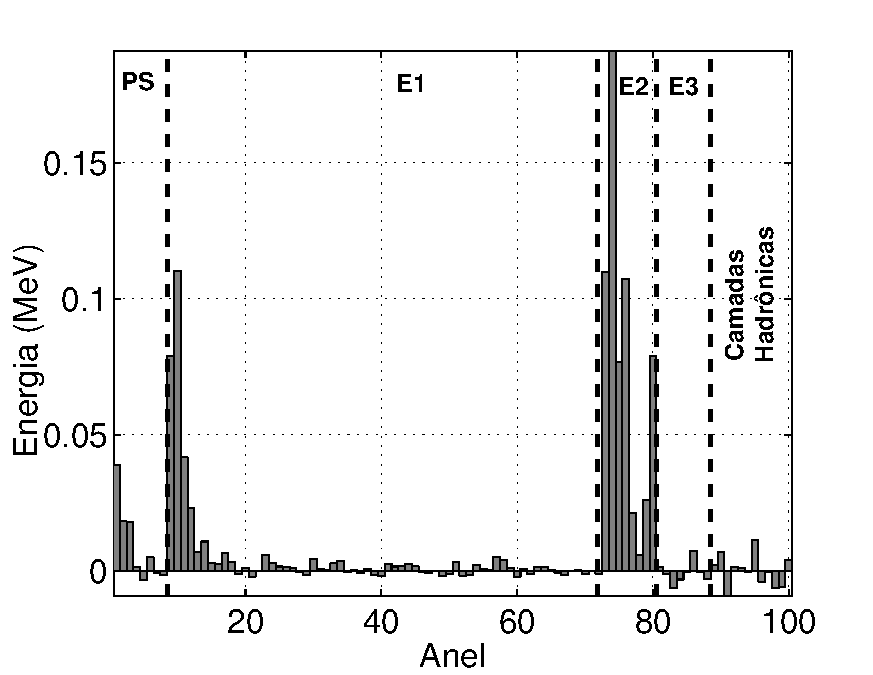
\epsfig{file=cap3_jet_ele,width=7.5cm}}
  \vspace{.3cm}
  \centerline{(c)}\medskip
\end{minipage}
\caption{Sinais em an�is para (a) el�tron t�pico, (b) jato t�pico e
(c) jato com perfil semelhante ao de el�trons.} \label{fig_sig_anel}
\end{figure}

Antes da utiliza��o nos sistemas de classifica��o (teste de
hip�tese) os sinais em an�is s�o normalizados dividindo-se a energia
de cada anel pela energia total do evento:
\begin{equation}
 r_i=\frac{r_i}{\sum_{i=1}^{100}r_i}
\end{equation}

\subsection{Normaliza��o}

Os sinais em an�is s�o normalizados fazendo-se...

\subsection{Teste de Hip�teses - Classificador Neural}

Para o processo de discrimina��o propriamente dito (teste de hip�teses), o Neural Ringer utiliza um classificador neural supervisonado 
na arquitetura Perceptron de M�ltiplas Camadas (MLP \textit{Multi-Layer Perceptron})~\cite{haykin:nn:2008}. Os 
classificadores neurais s�o capazes de produzir superf�cies n�o-lineares de separa��o, aumentando a efici�ncia 
de discrimina��o quando comparados aos classificadores lineares. Devido a sua estrutura paralelamente distribu�da, 
� capaz de responder rapidamente quando um padr�o de entrada � aplicado. Considerando as caracter�sticas expostas 
(alta efici�ncia e processamento r�pido) os classificadores neurais s�o adequados ao ambiente do segundo n�vel de 
filtragem \textit{online} do ATLAS.

\subsection{Tempo de Execu��o}

Um aspecto crucial dos algoritmos para o sistema filtragem online � o tempo de execu��o. No caso do 
\textit{Neural Ringer}, que � um algoritmo para o segundo n�vel de filtragem, a janela de tempo m�xima permitida �
de 40 ms. Uma an�lise detalhada do tempo de processamento requerido pelo \textit{Neural Ringer} foi realizada no 
trabalho \cite{tese:torres:2010}. ...

\section{Extens�es ao Neural Ringer}

Com efici�ncia mais alta que o algoritmo padr�o (T2Calo) e tempo de processamento dentro da janela aceita para o 
L2, o discriminador Neural Ringer mostrou-se uma op��o bastante interessante para o problema da filtragem 
\textit{online} de el�trons no ATLAS. Trabalhos v�m sendo desenvolvidos com o objetivo de melhorar a efici�ncia 
do Neural Ringer com a adi��o de uma etapa de pr�-processamento ao classificador neural 
(ver Figura \ref{fig_ringerext}), na qual, os sinais em an�is s�o mapeados em um conjunto (em geral mais compacto) 
de caracter�sticas discriminantes. A seguir estes trabalhos ser�o descritos brevemente.


\begin{figure} \centering
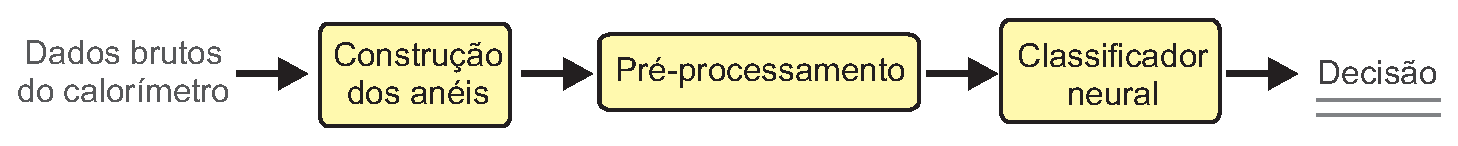
\includegraphics[width=15cm]{cap3_ringerext}
\caption{Fluxo de processamento das extens�es ao \textit{Neural Ringer}.} \label{fig_ringerext}
\end{figure}


\subsection{Pr�-processamento linear}

Embora a constru��o dos an�is j� seja respons�vel por uma consider�vel redu��o de dimens�o (por um fator de 10 vezes), 
no trabalho \cite{tese:herman:2006} foi realizado um estudo detalhado a respeito da utiliza��o da An�lise de 
Componentes Principais (PCA - \textit{Principal Component Analysis}) para compacta��o. A PCA foi aplicada aos 
sinais em an�is e o classificador neural treinado a partir das componentes principais estimadas. Com a PCA, 
foi alcan�ado um fator de redu��o de aproximadamente 4 vezes, mantendo desempenho semelhante ao Neural Ringer 
tradicional. Visando melhorar explorar toda a granularidade e segmenta��o dispon�vel aos calor�metros do ATLAS, 
foi proposta a realiza��o do processo de compacta��o de modo segmentado (a n�vel de cada camada do calor�metro).

No trabalho \cite{tese:torres:2010}, foi utilizada uma t�cnica de compacta��o mais adequada a problemas de 
classifica��o, a PCD (\textit{Principal Components for Discrimination}, ou em portugu�s Componentes Principais 
de Discrimina��o).  Foi realizado tamb�m um estudo referente � aplica��o da An�lise de Componentes Independentes 
(ICA \textit{Independent Component Analysis}) como uma etapa adicional de pr�-processamento, aparecendo logo 
ap�s a compacta��o. Os resultados mostraram que a combina��o de ICA e PCD foi capaz de melhorar o desempenho 
em rela��o ao Neural Ringer, sem modificar significativamente o tempo de processamento necess�rio para a tomada 
de decis�o.


\subsection{Pr�-processamento n�o-linear}

Conforme descrito no Cap�tulo 2, os calor�metros, embora projetados para serem detectores lineares na 
identifica��o de el�trons, na pr�tica, seu comportamento � n�o-linear, devido a fen�menos como satura��o 
de sensores, atenua��o da luz (em calor�metros cintilantes), etc. Ent�o, talvez uma t�cnica n�o-linear 
de extra��o de caracter�sticas seja mais adequada ao problema.

Os trabalhos desenvolvidos anteriormente utilizam apenas t�cnicas lineares como PCA, PCD e ICA. Os estudos 
desenvolvidos durante a elabora��o desta tese tiveram o objetivo de investigar a aplica��o da vers�o 
n�o-linear da an�lise de componentes independentes (NLICA) para extra��o de caracter�sticas no segundo 
n�vel de filtragem \textit{online} de el�trons do ATLAS. Considerando que existem diversos algoritmos 
para a estima��o da NLICA, neste trabalho foram realizados estudos com alguns destes m�todos. Os diversos 
modelos foram comparados considerando efici�ncia de discrimina��o e tempo de processamento necess�rio para 
produzir a decis�o.






    \chapter{An�lise de Componentes Independentes}
\label{cap_ica}

Neste cap�tulo, ser�o mostradas, de modo resumido, as principais caracter�sticas dos modelos
linear e n�o-linear da an�lise de componentes independentes (respectivamente ICA e NLICA).
Tamb�m ser�o brevemente apresentados os algoritmos utilizados para estima��o da NLICA no contexto
deste trabalho. A seguir, ser� realizada uma revis�o bibliogr�fica das aplica��es da an�lise de
componentes independentes em problemas de extra��o de caracter�sticas, dando enfoque especial a
F�sica de Altas Energias (HEP - \textit{High-Energy Physics}). Em complementa��o a este Cap�tulo,
no Ap�ndice~\ref{apend_fex}, s�o apresentados, de modo mais detalhado
(com um maior formalismo matem�tico), alguns dos algoritmos mais utilizados na literatura para ICA/NLICA,
juntamente com os diversos
par�metros empregados nesta rotinas para estimar o grau de independ�ncia entre os sinais.

\section{Modelo Linear da ICA}

Em muitos problemas de processamento de sinais multi-dimensionais
\footnote{Sinais multi-dimensionais s�o, em geral, produzidos por sistemas de medi��o com
m�ltiplos sensores, mas tamb�m podem surgir a partir da aplica��o de transforma��es (como a transformada de
Fourier ou Wavelet) a sinais uni-dimensionais.} deseja-se encontrar uma transforma��o que, de algum modo, torne a
estrutura essencial dos dados mais acess�vel~\cite{book:oja:2001}.
Entre as t�cnicas lineares que buscam, atrav�s
de premissas distintas, por uma nova representa��o para os sinais
multi-dimensionais, pode-se mencionar a An�lise de Componentes Principais (PCA
- \textit{Principal Component Analysis})~\cite{book:pca:2002}, a
An�lise de Fatores (\textit{Factor
Analysis})~\cite{book:factor:1967} e a An�lise de Componentes
Independentes (ICA - \textit{Independent Component
Analysis})~\cite{book:oja:2001}.

Entre as t�cnicas listadas acima, a an�lise de componentes
independentes busca por uma transforma��o onde os componentes na sa�da s�o
estatisticamente independentes. A ICA v�m sendo aplicada na
solu��o de diversos problemas na �rea de processamento de sinais
como cancelamento de ru�do~\cite{article:ica:noisecan}, sonar
passivo~\cite{article:moura:sonarbook},
telecomunica��es~\cite{article:icateleco:2007}, reconhecimento
facial~\cite{article:icaface:2007} e
biom�dica~\cite{article:icabio:2007}.

\begin{itemize}
\item \textbf{Independ�ncia Estat�stica}: Considerando duas
vari�veis aleat�rias (VAs) $y_1$ e $y_2$, se elas s�o
independentes, ent�o o conhecimento de uma n�o traz nenhuma
informa��o a respeito da outra. Matematicamente, $y_1$ e $y_2$ s�o
independentes estatisticamente se e somente se
\cite{Book:Papoulis:1991}:
\begin{equation}\label{indep1}
    p_{y1,y2}(y_1,y_2)=p_{y1}(y_1)p_{y2}(y_2),
\end{equation}
\\
onde $p_{y1,y2}(y_1,y_2)$, $p_{y1}(y_1)$ e $p_{y2}(y_2)$ s�o
respectivamente as fun��es de densidade de probabilidade (pdf -
\textit{probability density function}) conjunta e marginais de
$y_1$ e $y_2$ \cite{Book:Papoulis:1991}.

Pode-se obter uma express�o equivalente � equa��o (\ref{indep1})
se, para todas as fun��es $g(y_1)$ e $h(y_2)$ absolutamente
integr�veis em $y_1$ e $y_2$, vale a igualdade:
\begin{equation}\label{indep2}
    \mathcal{E}\{g(y_1)h(y_2)\}=\mathcal{E}\{g(y_1)\}\mathcal{E}\{h(y_2)\}
\end{equation}
\\
Considerando que a estima��o das fun��es de densidade de probabilidade (necess�rias na equa��o (\ref{indep1})) � um
problema de dif�cil solu��o, pois, em geral os componentes independentes s�o desconhecidos,
uma vantagem da equa��o~(\ref{indep2}) � que as pdfs n�o s�o necess�rias. A defini��o de
independ�ncia pode ser facilmente estendida para mais de duas
vari�veis aleat�rias. Percebe-se que a
independ�ncia � um princ�pio mais restritivo que a descorrela��o
(quando $g(x)=x$ e $h(y)=y$). O conceito de
independ�ncia envolve o conhecimento de toda a estat�stica dos
dados, sendo assim muito mais abrangente que a descorrela��o
(utilizada pela PCA), que somente utiliza estat�stica de segunda
ordem (vari�ncia). %No Ap�ndice \ref{apend_fex} ser�o
%detalhados os princ�pios matem�ticos mais utilizados para a
%estima��o dos componentes independentes.
\end{itemize}

Na ICA, considera-se que um sinal multi-dimensional
$\mathbf{x}(t)=[x_1(t),...,x_N(t)]^T$ observado (ou medido) �
gerado a partir da combina��o linear das fontes independentes
$\mathbf{s}(t)=[s_1(t),...,s_N(t)]^T$. Na forma matricial e
suprimindo-se o �ndice temporal t, pode-se escrever
\cite{book:amari:2002}:
\begin{equation}\label{ica_eq}
\left[\begin{array}{c}
x_1(t)\\
\vdots \\
x_N(t)
\end{array}\right]=
\underbrace{\left[\begin{array}{c c c}
a_{11} & \dots & a_{1N}\\
\vdots & \ddots & \vdots\\
a_{N1} & \dots & a_{NN}
\end{array}\right]}_{\mathbf{A}} \times
\left[\begin{array}{c}
s_1(t)\\
\vdots \\
s_N(t)
\end{array}\right],
\end{equation}
ou na forma matricial (omitindo o �ndice temporal):
\begin{equation}\label{icamatrix}
\mathbf{x}=\mathbf{As},
\end{equation}
\\
onde $\mathbf{A}$ � a matriz de mistura.

O objetivo final da ICA � encontrar uma aproxima��o $\mathbf{y}$
das fontes independentes,
utilizando apenas os sinais observados $\mathbf{x}$. O vetor
$\mathbf{y}$ � definido por:
\begin{equation}\label{ica_inv}
 \mathbf{y}=\mathbf{Wx},
\end{equation}
sendo $\mathbf{W}$ a matriz de separa��o. Se $\mathbf{W}=\mathbf{A}^{-1} \rightarrow \mathbf{y}=\mathbf{s}$,
ent�o o problema foi completamente solucionado.

Um problema cl�ssico que pode ser solucionado usando-se ICA �
conhecido como \textit{cocktail-party
problem}~\cite{book:oja:2001}, e est� formulado de forma
simplificada, omitindo atrasos temporais e outros fen�menos
f�sicos, como a exist�ncia de m�ltiplas reflex�es, nas equa��es
(\ref{cpp}) e (\ref{ccp2}) (ver Figura \ref{cocktail}).
Considerando que numa sala existem duas pessoas falando
simultaneamente e dois microfones em diferentes posi��es, os
sinais gravados $x_1(t)$ e $x_2(t)$ s�o uma soma ponderada das
fontes $s_1(t)$ e $s_2(t)$:
\begin{eqnarray}\label{cpp}
% \nonumber to remove numbering (before each equation)
  x_1(t)=a_{11}s_1(t)+a_{12}s_2(t) \\
  \label{ccp2} x_2(t)=a_{21}s_1(t)+a_{22}s_2(t);
\end{eqnarray}
\\
os coeficientes $a_{ij}$ dependem das dist�ncias dos microfones �s
pessoas, e s�o os elementos da matriz de
mistura $\mathbf{A}$, onde:

\begin{equation}\label{matrizA}
    \mathbf{A}=\left[
                 \begin{array}{cc}
                   a_{11} &a_{12} \\
                   a_{21} & a_{22} \\
                 \end{array}
               \right].
\end{equation}

\begin{figure}[th]
\centering
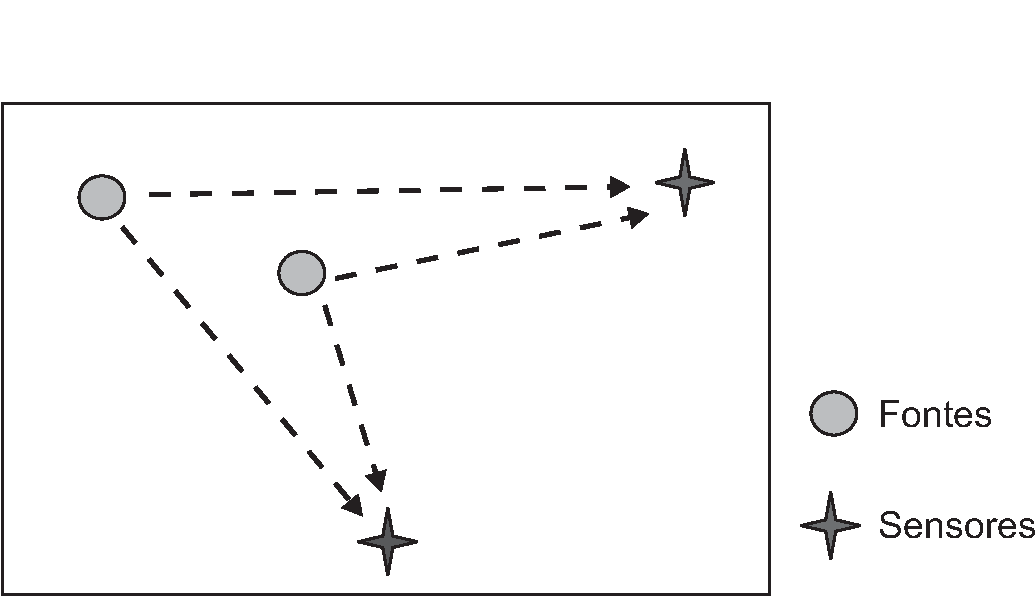
\includegraphics[width=9cm]{cap3_cocktail}
\caption{Diagrama do \textit{cocktail party problem}.}
\label{cocktail}
\end{figure}

Em um exemplo de aplica��o da ICA, a Figura \ref{sinais}-a mostra
as fontes $s_1(t)$ e $s_2(t)$, que foram misturadas linearmente,
gerando os sinais $x_1(t)$ e $x_2(t)$ da Figura \ref{sinais}-b.
Ap�s a aplica��o de um algoritmo para extra��o das componentes
independentes (FastICA \cite{article:hyvarinen:2000}), foram
obtidas as curvas da Figura \ref{sinais}-c. Percebe-se que os
sinais recuperados s�o c�pias dos originais, a menos de fatores
multiplicativos. Esta � uma das limita��es inerentes ao modelo da
ICA, n�o h� como garantir o fator de escala (que pode ser positivo
ou negativo) ou a ordem de extra��o dos componentes.

\begin{figure}[h!]
\begin{minipage}[b]{.48\linewidth}
  \centering
 \centerline{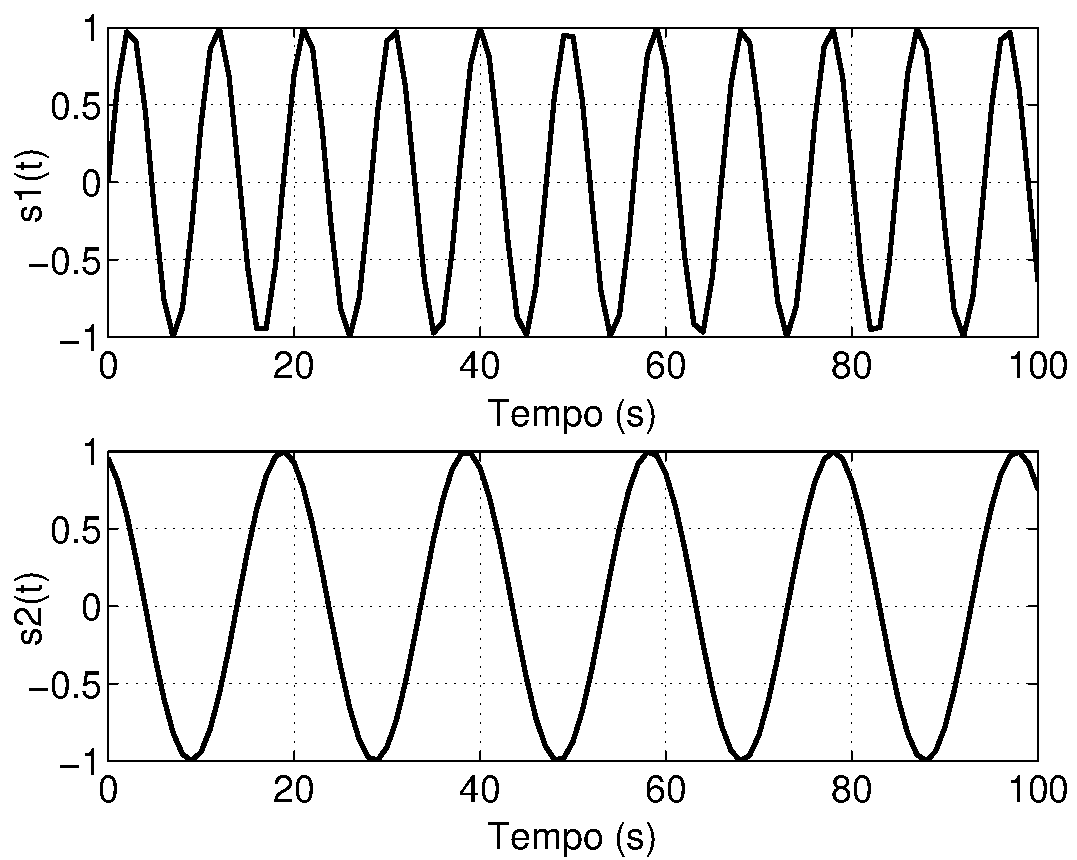
\epsfig{file=cap3_fontes,width=7.5cm}}
  \vspace{.3cm}
  \centerline{(a)}\medskip
\end{minipage}
\hfill
\begin{minipage}[b]{0.48\linewidth}
  \centering
 \centerline{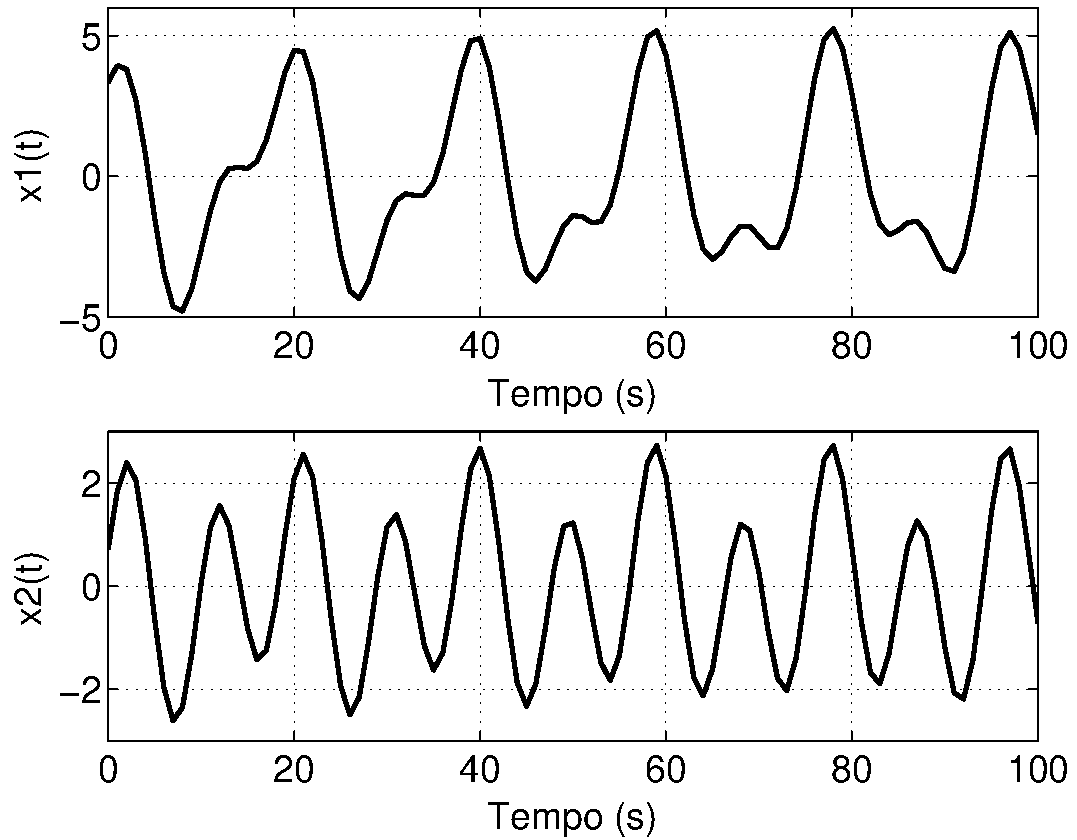
\epsfig{file=cap3_mix,width=7.5cm}}
  \vspace{.3cm}
  \centerline{(b)}\medskip
\end{minipage}
\hfill \linebreak
\begin{minipage}[b]{0.98\linewidth}
  \centering
 \centerline{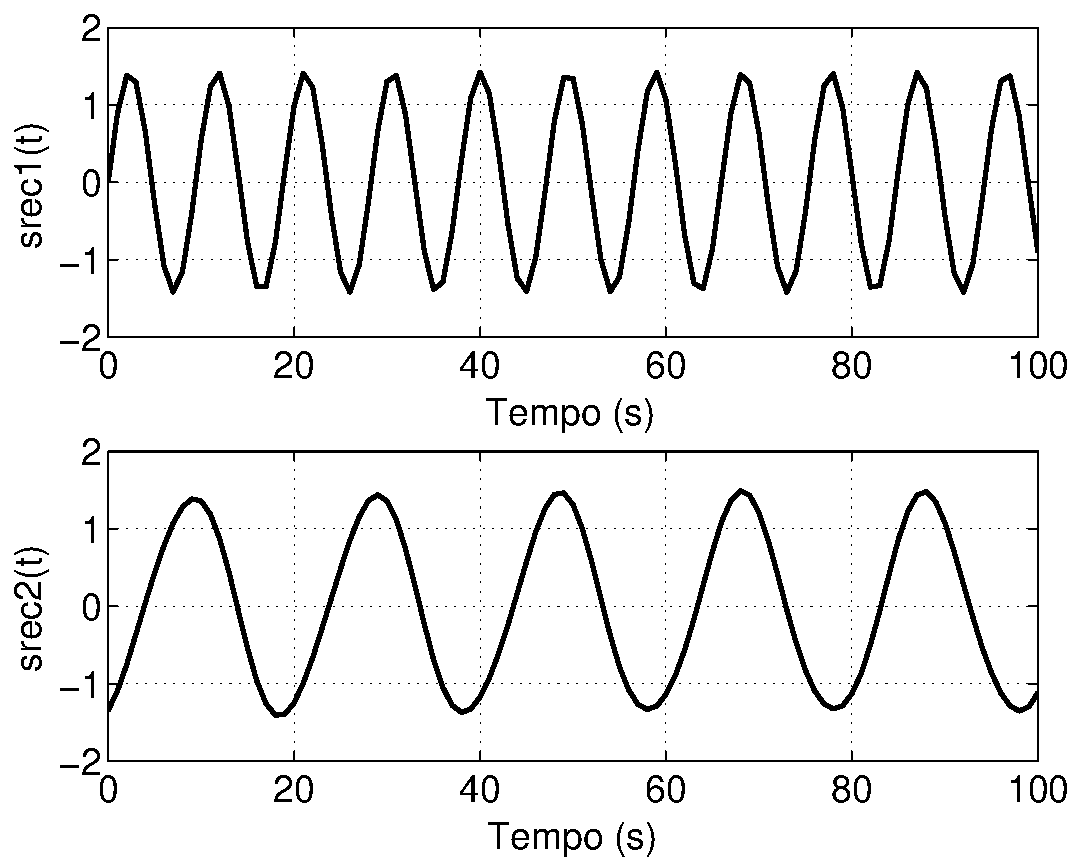
\epsfig{file=cap3_rec,width=7.5cm}}
  \vspace{.3cm}
  \centerline{(c)}\medskip
\end{minipage}
\caption{Sinais (a) fonte, (b) observados e (c) recuperados
atrav�s da ICA.} \label{sinais}
\end{figure}

%\begin{figure}[t!]
%\begin{center}
%\subfigure[]{\label{fontes}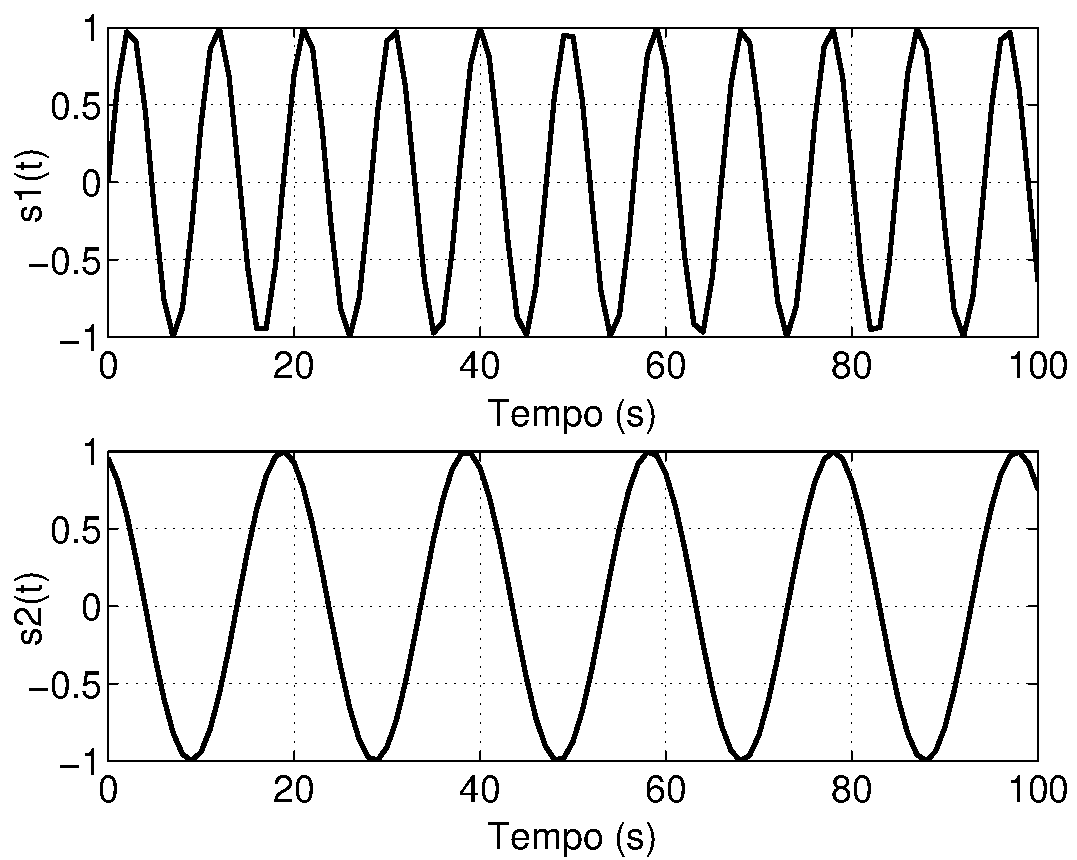
\epsfig{file=cap3_fontes,width=7.5cm,clip=}}
%\subfigure[]{\label{misturas}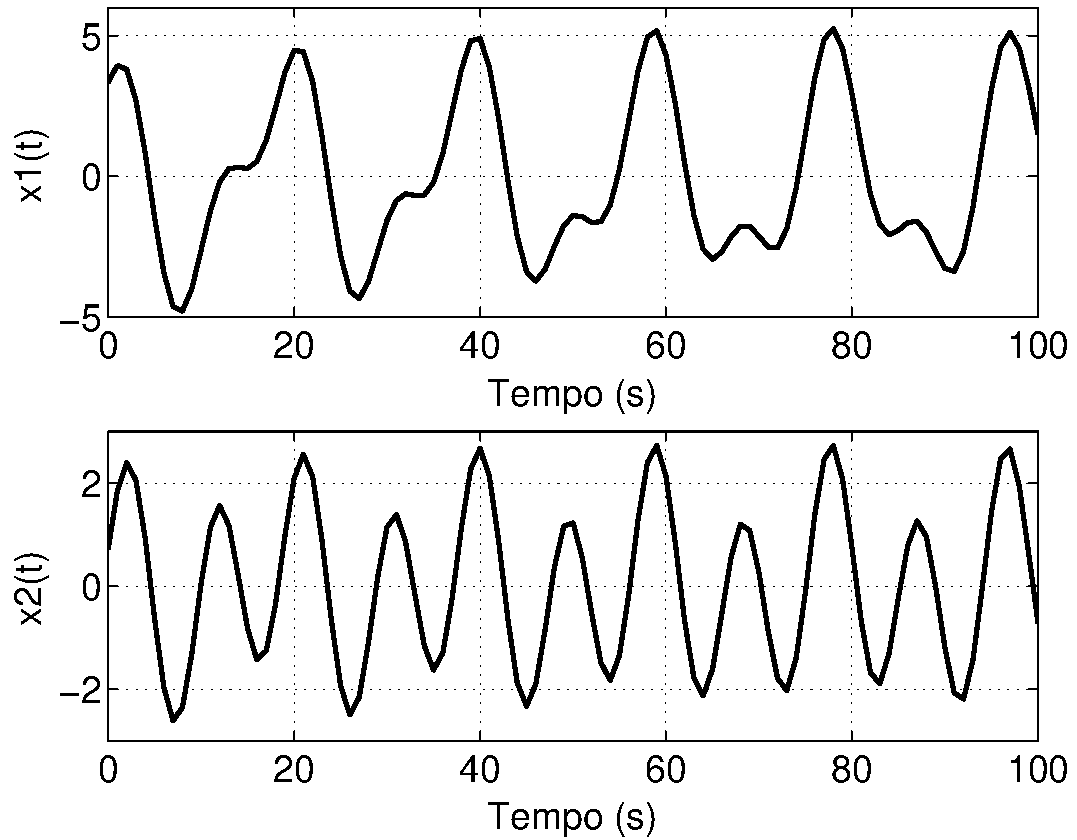
\epsfig{file=cap3_mix,width=7.5cm,clip=}}
%\subfigure[]{\label{recuperados}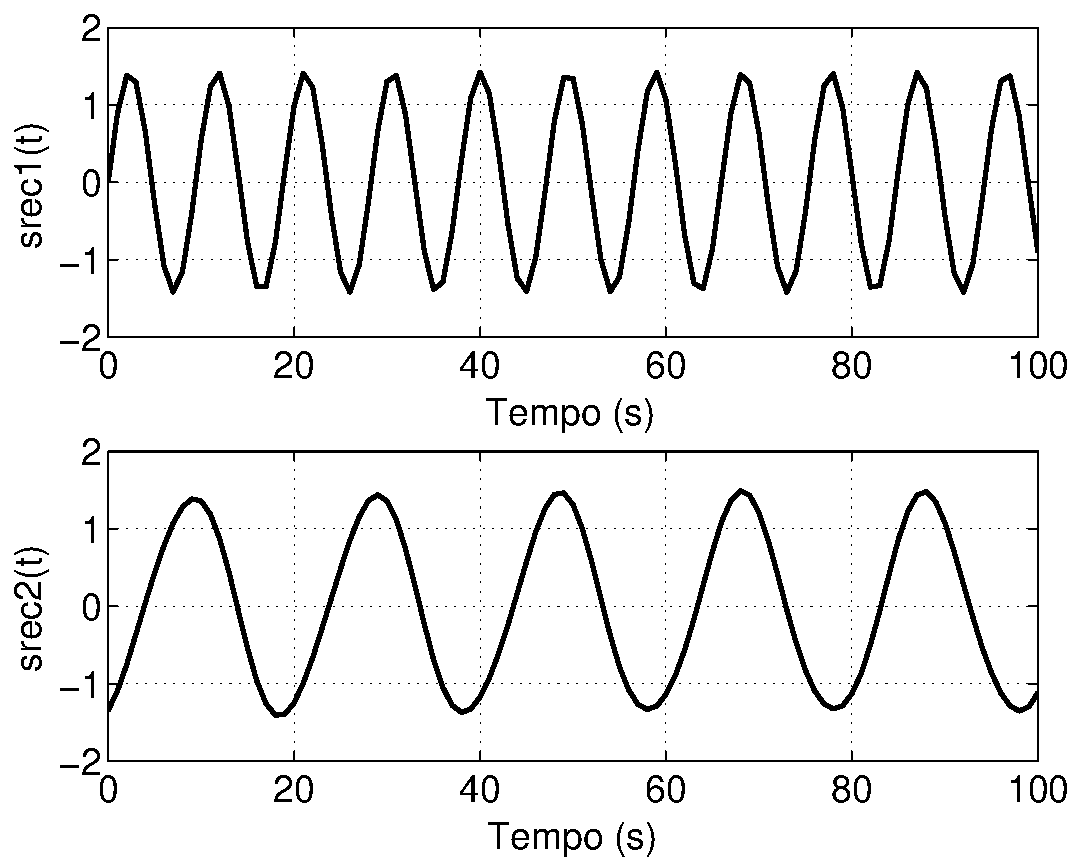
\epsfig{file=cap3_rec,width=7.4cm,clip=}}
%\end{center}
%\caption{Sinais (a) fonte, (b) observados e (c) recuperados atrav�s
%da ICA.}
%\end{figure}

As t�cnicas de ICA foram desenvolvidas inicialmente para
solucionar pro\-blemas de separa��o cega de sinais (BSS -
\textit{Blind Signal Separation}) semelhantes ao
\textit{cocktail-party problem}, por�m, mais recentemente,
surgiram outras aplica��es interessantes, como extra��o de
caracter�sticas, separa��o de fontes em telecomunica��es e redu��o
de ru�do em imagens \cite{book:oja:2001,article:hyvarinen:2000}.
Atualmente, ICA � aplicada com sucesso tanto para separa��o de
sinais como para extra��o de caracter�sticas.

\section{ICA N�o-Linear}

Em muitos problemas pr�ticos, o modelo b�sico da ICA, onde os
sinais observados s�o considerados combina��es lineares e
instant�neas das fontes, n�o representa corretamente o cen�rio
real.

A equa��o (\ref{nlica}) apresenta um modelo geral para as misturas
n�o-lineares:
\begin{equation}\label{nlica}
    \mathbf{x}=\mathbf{F}(\mathbf{s}),
\end{equation}
\\
onde $\mathbf{F}(.)$ � um mapeamento n�o-linear de $\mathbb{R}^N
\rightarrow \mathbb{R}^N$, $\mathbf{x}$ e $\mathbf{s}$ s�o
respectivamente os sinais observados e as fontes. A ICA n�o-linear
consiste em encontrar o mapeamento $\mathbf{G}(.)$: $\mathbb{R}^N
\rightarrow \mathbb{R}^N$ tal que os componentes de $\mathbf{y}$
sejam estatisticamente
independentes~\cite{article:simas:2007:lnlm}:
\begin{equation}\label{nlica2}
    \mathbf{y}=\mathbf{G}(\mathbf{x}).
\end{equation}

Uma caracter�stica da NLICA � que o problema apresenta m�ltiplas
solu��es~\cite{jutten:nlica:2003}. Se $\mathbf{y_1}$ e
$\mathbf{y_2}$ s�o vari�veis aleat�rias independentes, � f�cil
provar que $f(\mathbf{y_1})$ e $g(\mathbf{y_2})$ (onde $f(.)$ e
$g(.)$ s�o fun��es diferenci�veis) s�o tamb�m independentes
\cite{article:hyvarinen:1999}. Fica claro que, numa dada
aplica��o, sem o uso de restri��es adequadas, infinitos
mapeamentos inversos $\mathbf{G}$ satisfazem a condi��o de
independ�ncia entre os sinais estimados $y_i$, i=1,...,N. Se o
objetivo do problema for realizar a separa��o das fontes de modo
n�o-supervisionado ou cego (do ingl�s \textit{Blind Signal
Separation} - BSS), neste caso, deseja-se que os componentes $y_i$
sejam aproxima��es das fontes independentes ($\mathbf{s}$) que
produziram os sinais observados ($\mathbf{x}$). Ent�o, informa��es
a respeito do modelo de mistura ou das fontes devem ser conhecidas
a priori. A NLICA vem sendo aplicada com sucesso em problemas como
processamento de sinais de fala
\cite{article:rojas:ica:2003,article:miyabe:2009}, processamento
de imagens~\cite{article:allinson:2002,article:almeida:2008},
predi��o de s�ries de a��es em bolsas de
valores~\cite{article:chi:2009} e processamento de sinais de um
\textit{array} de
sensores~\cite{article:sensornlica:2007,app:nlica:qui}.

Em geral, o n�mero de par�metros a serem estimados num modelo de
ICA n�o-linear � maior do que no caso linear. Os algoritmos de
NLICA, se comparados aos de ICA, apresentam maior complexidade
computacional e converg�ncia mais lenta~\cite{jutten:nlica:2003}.
Considerando estas limita��es, nas aplica��es
de NLICA deve-se verificar se existem restri��es quanto ao aumento
do custo computacional no processo de estima��o dos componentes.
Em problemas de separa��o cega de fontes, o algoritmo a ser
utilizado deve ser esco\-lhi\-do utilizando informa��es a respeito
do modelo de mistura.

Entre os algoritmos de NLICA propostos na literatura, uma classe
de m�todos imp�e restri��es estruturais ao modelo de mistura.
Neste caso, pode-se garantir que os componentes estimados s�o
aproximadamente iguais �s fontes (a menos das indetermina��es de
fator multiplicativo e ordem de estima��o dos sinais, assim como
ocorre no modelo linear). Existem tamb�m alguns m�todos (ou
algoritmos) que n�o imp�em restri��es ao modelo de mistura, neste
caso, o mapeamento n�o-linear dos dados observados em componentes
independentes n�o garante a separa��o das fontes. Outro m�todo
diretamente relacionado com a NLICA, chamado de ICA Local, prop�e
uma etapa de agrupamento dos sinais em conjuntos de
caracter�sticas semelhantes, que deve ser realizada antes da ICA.
O agrupamento produz um mapeamento n�o-linear dos dados e a ICA
(linear) estima os componentes independentes. Mais informa��es a
respeito dos diversos algoritmos e modelos de NLICA ser�o
fornecidas nas pr�ximas se��es.

\subsection{Unicidade da Solu��o em NLICA} \label{seq_uni}

Conforme mencionado anteriormente, no caso n�o-linear, a independ�ncia estat�stica n�o � suficiente
para garantir a sepa\-ra��o das fontes. Se duas vari�veis
aleat�rias $y_1$ e $y_2$ s�o independentes, ent�o
$p_{y1,y2}(y_1,y_2)=p_{y1}(y_1)p_{y2}(y_2)$. Para fun��es
diferenci�veis $f$ e $g$, pode-se provar
que~\cite{article:jutten:1999}:
\begin{equation}\label{uniq}
    p_{f(y_1),g(y_2)}(y_1,y_2)=p_{f(y_1)}(y_1)p_{g(y_2)}(y_2),
\end{equation}
e ent�o as vari�veis $f(y_1)$ e $g(y_2)$ s�o tamb�m independentes.
Esta indetermina��o, diferente do fator de escala e da ordem de
estima��o dos componentes (que s�o inerentes a ICA linear), n�o
s�o aceit�veis em um problema de separa��o de fontes.

Estudos te�ricos indicaram que a unicidade da solu��o da NLICA
pode ser conseguida se o problema apresentar pelo menos uma das
caracter�sticas a seguir \cite{article:hyvarinen:1999}:

\begin{itemize}
    \item O n�mero de componentes � igual a dois. Deste modo, os sinais podem ser considerados como uma vari�vel complexa.
    \item As pdf dos componentes independentes s�o limitadas a valores conhecidos.
    \item O mapeamento $\mathbf{F}$ preserva o zero ($\mathbf{F}(0)=0$) e � un�voco.
    \item O modelo de mistura � conhecido a priori e utilizado como informa��o para o algoritmo de estima��o das componentes independentes.
\end{itemize}


\subsection{Modelos com Restri��es Estruturais}

Um caso especial da ICA n�o-linear s�o os m�todos de estima��o dos componentes independentes que
utilizam informa��es a respeito do modelo n�o-linear que gerou os dados
observados. Estas informa��es se configuram em restri��es
estruturais ao mapeamento inverso (que � estimado pelo algoritmo).
Entre os modelos com restri��es estruturais pode-se destacar o de misturas
\textbf{p�s n�o-lineares} (PNL), que ser� descrito a seguir.

\subsubsection{Misturas P�s N�o-Lineares}

O modelo de misturas p�s n�o-lineares~\cite{article:jutten:1999} �
um dos mais utilizados na lite\-ra\-tura, com aplica��es em
processamento de
fala~\cite{article:rojas:nlica:2004,ica:ap_pnl:2004}, separa��o de
sinais de �udio~\cite{ica:ap_pnl:2007,article:solazzi:pnl:2004} e
processamento de imagens \cite{article:pnlimage:2007}.

No modelo PNL, considera-se que inicialmente ocorre uma combina��o
linear das fontes (como no modelo b�sico de ICA), e as fun��es
n�o-lineares $f_i$ s�o aplicadas antes da observa��o dos sinais
$x_i$:
\begin{equation}\label{pnlin}
    x_i=f_i\Big(\sum_{j=1}^n a_{ij}s_j \Big).
\end{equation}
� importante notar que as n�o-linearidades s�o aplicadas
individualmente a cada componente da mistura linear (n�o s�o
permitidas n�o-linearidades cruzadas). A Figura~\ref{fig_pnl} ilustra
o modelo de misturas PNL.

\begin{figure}[th]
\centering
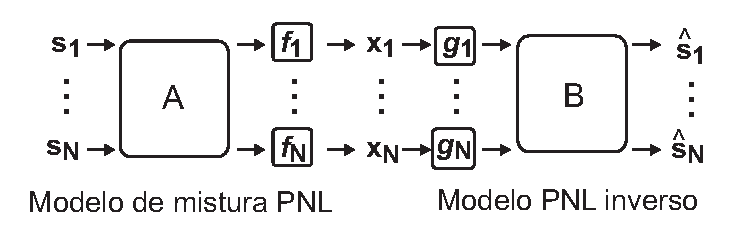
\includegraphics[width=10cm]{cap3_pnl}
\caption{Diagrama do modelo de mistura PNL.} \label{fig_pnl}
\end{figure}

A considera��o de que as misturas s�o p�s n�o-lineares permite uma
grande simplifica��o do problema, e as indetermina��es existentes
se tornam semelhantes �s do caso linear. A modelagem atrav�s da
equa��o (\ref{pnlin}) satisfaz grande parte dos fen�menos
n�o-lineares, como, por exemplo, a modelagem da distor��o de
sensores num meio de propaga��o linear.

Diversos algoritmos foram propostos na literatura para estima��o
do modelo PNL. Um dos primeiros
trabalhos~~\cite{article:jutten:1999}, utiliza redes neurais para
estimar cada fun��o n�o-linear $g_i$ e o ajuste dos pesos � feito
a partir da minimiza��o da informa��o m�tua usando o m�todo do
gradiente (mais detalhes a respeito deste algoritmo podem ser
encontrados no Ap�ndice \ref{apend_fex}). Na estima��o do modelo
PNL usando um algoritmo do tipo gradiente descendente (que realiza
uma busca local), o grande n�mero de par�metros e as
caracter�sticas n�o-lineares do problema contribuem para a
converg�ncia em m�nimos locais. Visando minimizar esta limita��o,
foram propostos algoritmos de estima��o do modelo PNL usando
m�todos de busca global como algoritmos
gen�ticos~\cite{article:kai:2006,article:nlica_ga:2001},
recozimento simulado (\textit{Simulated Annealing}) e aprendizado
competitivo (\textit{Competitive
Learning})~\cite{article:rojas:nlica:2004}.

\subsubsection{Outros Modelos de Misturas com Restri��es Estruturais}

Alguns modelos com restri��es estruturais diferentes do PNL foram
propostos na literatura. No trabalho
\cite{article:solazzi:pnl:2004}, o modelo de mistura � definido
por:
\begin{equation}\label{eq_pnll}
    \mathbf{x}=\mathbf{A_2}f(\mathbf{A_1}\mathbf{s}),
\end{equation}
sendo $\mathbf{A_1}$ e $\mathbf{A_2}$ matrizes quadradas e
$f=[f_1,f_2,...,f_N]^T$ um mapeamento com fun��es n�o-lineares aplicadas a cada
componente (assim como o modelo PNL, este tamb�m n�o permite
n�o-linearidades aplicadas a mais de um componente). O modelo
definido na Equa��o \ref{eq_pnll} e ilustrado tamb�m na Figura
\ref{fig_pnll} � chamado P�s N�o-linear Linear (PNL-L). O bloco
linear $\mathbf{A_2}$ � executado ap�s a aplica��o das fun��es
n�o-lineares, produzindo um modelo mais geral que o PNL. Nos
trabalhos \cite{article:woo:nl2005,article:gao:nl2005} s�o
propostos algoritmos baseados em redes neurais para a estima��o do
modelo PNL-L.

\begin{figure}[th]
\centering
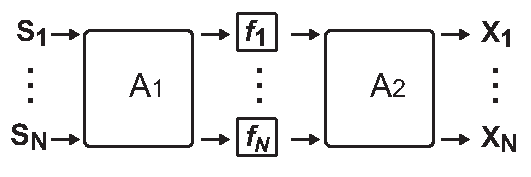
\includegraphics[width=7cm]{cap3_pnll}
\caption{Diagrama do modelo PNL-L.} \label{fig_pnll}
\end{figure}

Em \cite{article:gao:nl2005}, um modelo estrutural chamado mono
n�o-linearidade (ver Figura \ref{fig_mnlin}) foi proposto para o
problema da NLICA. Neste modelo os sinais observados s�o gerados a
partir de:
\begin{equation}\label{eq_mnlin}
    \mathbf{x}=f^{-1}(\mathbf{A}f(\mathbf{s})).
\end{equation}
Este modelo (chamado de mistura de mono
n�o-linearidade e ilustrado na Figura~\ref{fig_mnlin}) � dito mais geral que o PNL, pois as fun��es
n�o-lineares ($f_i$) podem ser aplicadas a mais de um componente. A an�lise deste
modelo, a partir da teoria da an�lise funcional (\textit{functional analysis})~\cite{book:function:1984}, mostra
que pode representar qualquer mistura com duas camadas de n�o-linearidades~\cite{article:gao:nl2005}.

\begin{figure}[th]
\centering
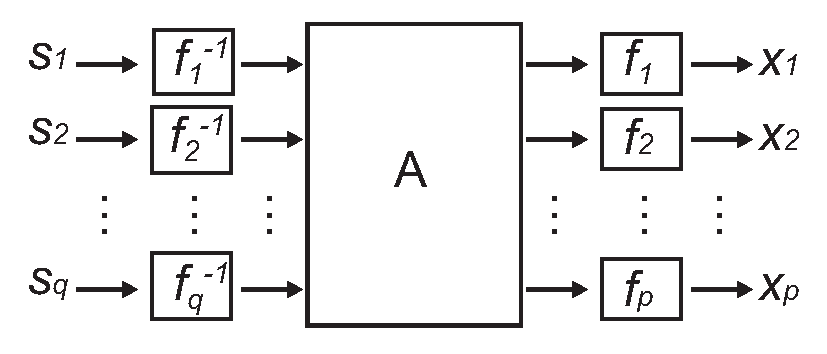
\includegraphics[width=8.5cm]{cap3_mononl}
\caption{Diagrama do modelo da Mono n�o-linearidade.}
\label{fig_mnlin}
\end{figure}

\subsection{Algoritmos sem Restri��es Estruturais}

Se nenhuma restri��o ao modelo de mistura � imposta, n�o h�
garantia que os componentes independentes estimados estejam
relacionados com as fontes (ver Se��o \ref{seq_uni}). Entre os
m�todos de NLICA sem restri��es estruturais, pode-se destacar o
uso de mapas auto-organiz�veis e os m�todos que utilizam
infer�ncia Bayesiana.

\subsubsection{NLICA a Partir de Mapas Auto-Organiz�veis}

Uma das primeiras tentativas bem-sucedidas de estimar o modelo da
NLICA foi realizada atrav�s de mapas auto-organiz�veis (SOM -
\textit{Self-Organizing Maps})~\cite{article:pajunen:1996}.
Pode-se provar que as coordenadas $y_1$ e $y_2$ do neur�nio
vencedor no mapa (ver Figura \ref{fig_som_nlica}) s�o
independentes e aproximadamente uniformemente distribu�das
\cite{article:pajunen:1996}. Para estimar a NLICA, o SOM �
treinado usando como entradas os sinais observados, e as
coordenadas do neur�nio vencedor correspondem a uma aproxima��o
discreta dos componentes independentes (o n�mero de n�veis
poss�veis sinal estimado � igual ao n�mero de neur�nios utilizados
para represent�-lo).

\begin{figure}[th]
\centering
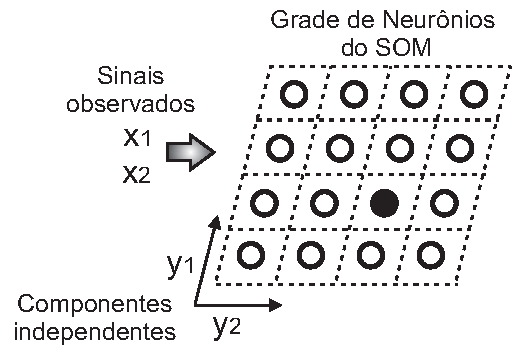
\includegraphics[width=8cm]{cap3_som_nlica}
\caption{NLICA a partir de SOM.} \label{fig_som_nlica}
\end{figure}

Entre as desvantagens do m�todo pode-se destacar
\cite{jutten:nlica:2003}:

\begin{itemize}
    \item O mapeamento � discreto (existe um n�mero limitado de neur�nios no mapa),
    ent�o, algum tipo de regulariza��o � necess�ria para produzir componentes cont�nuos.
    Esse problema pode ser minimizado aumentando-se o n�mero de neur�nios do mapa
(por�m, isto aumenta o custo computacional para estima��o do mapa).
    \item Os componentes a serem estimados devem ter pdf (fun��o densidade de probabilidade) sub-gaussiana
(quanto mais pr�xima da distribui��o uniforme, melhor).
    \item O custo computacional para treinamento dos mapas aumenta rapidamente com o n�mero de componentes independentes a serem estimados.
\end{itemize}

%Para avaliar o custo computacional, o n�mero de par�metros Np do
%SOM pode ser estimado pela express�o:
%\begin{equation}
%    Np=N \times (Q_L)^N
%\end{equation}
%onde $N$ � o n�mero de componentes a serem estimados (que �
%considerado igual ao n�mero de sinais observados) e $Q_L$ � o
%n�mero de n�veis de quantiza��o\cite{article:pnlimage:2007}
%desejado~\cite{article:simas:2007:lnlm}.

Diversas aplica��es do SOM para estima��o da NLICA podem ser
encontradas na literatura, entre elas pode-se citar os trabalhos
 e \cite{article:wang:somnlica:2007,article:allinson:2002,article:som:vizual:2003}, onde
o objetivos eram, respectivamente, separa��o de imagens
sobrepostas,remo��o de ru�do e visualiza��o de dados
multi-dimensionais.

Com uma formula��o alternativa aos SOM, o Mapeamento Topogr�fico
Generativo (GTM - \textit{Generative Topographic Mapping}) foi
introduzido em \cite{article:bishop:1998}, e apresenta princ�pios
estat�sticos mais fundamentados que o mapa SOM. O m�todo GTM
b�sico tem poucas vantagens pr�ticas em rela��o aos Mapas
Auto-Organiz�veis, pois aqui as componentes independentes tamb�m
s�o assumidas como processos uniformemente distribu�dos e o espa�o
de caracter�sticas � formado a partir de uma grade retangular
discreta m-dimensional. Por�m, devido a sua formula��o matem�tica,
o GTM pode ser estendido para vari�veis n�o
uniformes.

O trabalho \cite{article:pajunen:1997} prop�e uma
modifica��o � formula��o b�sica onde s�o introduzidos
coe\-fi\-cientes de pondera��o que permitem a estima��o de
componentes independentes com qualquer tipo de distribui��o. Os
componentes s�o modelados como misturas de sinais Gaussianos e os
par�metros s�o estimados usando o algoritmo \textit{Expectation
Maximization} \cite{article:hyvarinen:2000}. O treinamento do GTM
envolve dois passos, a avalia��o da probabilidade a
\textit{posteriori} e a adapta��o dos par�metros do modelo, neste sentido, o processo � semelhante ao
utilizado pela abordagem da infer�ncia Bayesiana, que ser� mostrada com mais detalhes a seguir.
N�o foram encontradas muitas aplica��es do GTM na estima��o da NLICA.

\subsubsection{NLICA a partir de Infer�ncia Bayesiana}

Nos m�todos baseados em infer�ncia Bayesiana, considera-se que os
sinais observados s�o gerados a partir
de~\cite{article:lappalainen:2000}:
\begin{equation}
    \mathbf{x}=f(\mathbf{s}) + \mathbf{n}
\end{equation}
onde $\mathbf{n}$ � definido como ru�do Gaussiano independente dos
componentes a serem estimados.

Neste contexto, os componentes independentes s�o modelados como misturas de sinais
de distribui��o Gaussiana.Pode-se provar que, dado um n�mero
suficiente de Gaussianas, qualquer distribui��o de
probabilidade pode ser aproximada~\cite{article:lappalainen:2000}. Uma varia��o deste
m�todo foi aplicada em \cite{article:lappalainen:bay1999} para o
mo\-de\-lo linear da ICA. Em grande parte dos algoritmos Bayesianos
para NLICA, redes neurais tipo MLP de duas camadas s�o treinadas
para aproximar o mapeamento n�o-linear, neste caso, t�m-se que~\cite{jutten:nlica:2003}:
\begin{equation}
    f(\mathbf{s})=\mathbf{B}\Phi(\mathbf{As}+\mathbf{a})+\mathbf{b}
\end{equation}

Em um m�todo de estima��o Bayesiano, probabilidades a
\textit{posteriori} s�o asso\-cia\-das a cada modelo n�o-linear que,
possivelmente, teria gerado os dados observados. Verificar uma
quantidade t�o grande de modelos n�o � poss�vel na pr�tica; ent�o,
os m�todos Bayesianos para NLICA utilizam uma t�cnica chamada de
``aprendizagem amostral" (EL - \textit{ensemble learning})
\cite{aricle:minskin:2000}. Na EL, somente o conjunto mais
prov�vel de modelos � testado utilizando uma aproxima��o
param�trica que � ajustada � probabilidade a \textit{posteriori}
\cite{article:valpola:2000ica}.

M�todos Bayesianos de NLICA foram propostos
em~\cite{article:honkela:2004ica} e \cite{article:honkela:2007}.
No trabalho~\cite{article:ilin:2004ie} foram realizados testes
experimentais para comparar o desempenho dos mode\-los Bayesiano e
p�s n�o-linear (PNL) na estima��o dos componentes independentes, as principais
conclus�es foram:
\begin{itemize}
    \item os algoritmos PNL apresentam desempenho superior quando as misturas
     seguem o modelo PNL cl�ssico (n�o-linearidades invers�veis e mesmo n�mero de componentes independentes e
     sinais observados);
    \item o desempenho de ambos os m�todos pode ser melhorada a partir da
    explora��o da informa��o de mais misturas que componentes independentes;
    \item a principal vantagem do m�todo Bayesiano � que mapeamentos mais
    gen�ricos podem ser produzidos (uma vez que n�o h� restri��es estruturais).
    Estes m�todos geralmente apresentam maior custo computacional e necessitam
    de v�rias inicializa��es para obter uma solu��o �tima (podem apresentar
    problemas com m�nimos locais da fun��o custo).
\end{itemize}

No trabalho \cite{app:nlica:qui} um algoritmo Bayesiano de NLICA
foi utilizado com sucesso para a separa��o de sinais medidos em um
conjunto de sensores qu�micos.

\subsubsection{O Algoritmo MISEP}

O algoritmo MISEP \cite{article:misep:2004} utiliza a minimiza��o
da Informa��o M�tua (ver Ap�ndice \ref{apend_fex}) como estrat�gia
para busca pelos componentes independentes. Esta rotina � considerada como
uma extens�o do m�todo INFOMAX \cite{book:oja:2001}, podendo ser
utilizado para estimar tanto o modelo linear quanto o n�o-linear
da ICA. Na Figura \ref{fig_misep} pode-se observar um diagrama do
MISEP (para duas entradas e duas sa�das), onde $x_i$ e $y_i$ s�o
respectivamente os sinais observados e os componentes
independentes estimados, o bloco $\mathbf{G(.)}$, no caso linear,
aproxima a matriz de separa��o $\mathbf{W}$, e para a NLICA, deve
fornecer uma aproxima��o do mapeamento n�o-linear inverso. As
fun��es n�o-lineares $\psi_i$ e as vari�veis de sa�da $z_i$ s�o
utilizadas apenas no processo de treinamento. Ap�s a converg�ncia
do algoritmo, as n�o-linearidades devem ser aproxima��es da fun��o
de probabilidade cumulativa (cdf - \textit{cumulative probability
function}) dos componentes independentes.

\begin{figure}[th]
\centering
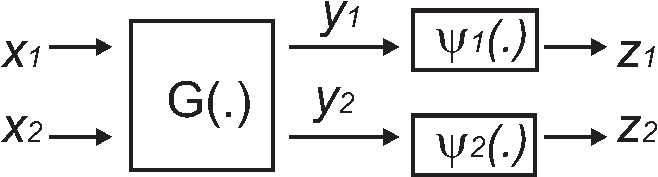
\includegraphics[width=7cm]{cap4_misep}
\caption{Diagrama do algoritmo MISEP.} \label{fig_misep}
\end{figure}

Para a aplica��o em NLICA, o bloco $\mathbf{G}(.)$ � estimado por
uma rede neural (que pode utilizar tanto a arquitetura
\textit{perceptron} de m�ltiplas camadas - MLP como rede de
fun��es de base radial - RBF). Como o objetivo � estimar a fun��o
de probabilidade cumulativa (cdf - \textit{cumulative distribution
function}), as sa�das $z_i$ s�o restritas ao intervalo [0,1] e as
$\psi_i$ s�o limitadas a fun��es estritamente crescentes. Para
estima��o iterativa de cada fun��o $\psi_i$, s�o utilizadas redes
neurais MLP com uma camada oculta (de neur�nios sigmoidais) e uma
camada de sa�da (linear). Estas redes tem uma entrada ($y_i$) e
uma sa�da ($z_i$). O treinamento do modelo MISEP � feito a partir
da maximiza��o da entropia das sa�das $z_i$, o que acaba
produzindo a minimiza��o da informa��o m�tua dos componentes
$y_i$, mais detalhes podem ser encontrados
em~\cite{article:misep:2004}

O MISEP foi aplicado em processamento de sinais de
�udio~\cite{article:misep:2004} e separa��o de imagens
\cite{article:Almeida05}. Foram propostas tamb�m, modifica��es ao
algoritmo MISEP visando otimizar a estima��o dos componentes
independentes quando as misturas seguem os modelos p�s n�o-linear
(PNL)~\cite{article:misep:pnl} e p�s n�o-linear-linear
(PNL-L)~\cite{article:misep:pnll}.


\subsection{ICA Local}

Considerando um problema onde o conjunto de sinais
multi-dimensionais apresenta grande varia��o em suas
caracter�sticas estat�sticas, o modelo linear da ICA pode n�o ser
capaz de representar adequadamente os dados. Neste contexto, pode
ser mais interessante tratar o conjunto de sinais de modo local,
ou seja, em subconjuntos onde os elementos tem caracter�sticas
semelhantes.

A ICA Local realiza a estima��o dos componentes independentes a partir de k subconjuntos dos dados
(ver Figura \ref{fig_local}). Conforme proposto em \cite{karhunen:local:1999}, um conjunto de
dados de alta dimens�o pode ser separado em sub-conjuntos (onde os elementos
apresentam caracter�sticas semelhantes), atrav�s
de algum algoritmo de agrupamento como o \textit{k-means}
\cite{book:duda:2000} ou SOM \cite{article:som:oja:1996}, e
modelos da ICA linear s�o ent�o estimados para cada
subconjunto. Caso n�o exista informa��o a priori a respeito do
n�mero de agrupamentos, metodologias foram propostas nos
trabalhos~\cite{article:cluster1:1999,article:cluster2:1998} para
sua estima��o.

\begin{figure}[bh]
\centering
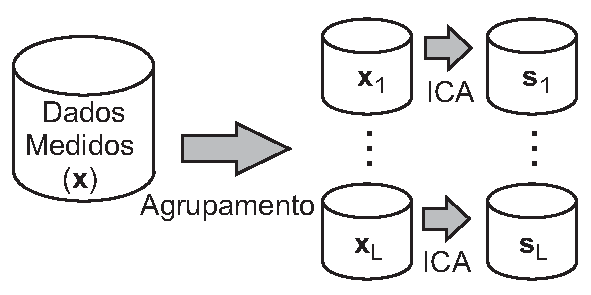
\includegraphics[width=8.5cm]{cap3_local}
\caption{Diagrama do modelo da ICA local.} \label{fig_local}
\end{figure}

Na ICA Local, o agrupamento � respons�vel por uma representa��o
n�o-linear dos dados, enquanto modelos de ICA linear aplicados a
cada sub-conjunto (\textit{cluster}) descrevem as caracter�sticas
locais. A ICA local pode ser considerada como um
compromisso entre os modelos linear e n�o-linear da ICA
\cite{jutten:nlica:2003}. O objetivo � obter uma melhor
representa��o dos dados (se comparado com o modelo linear da ICA),
evitando os problemas computacionais do modelo n�o-linear
\cite{karhunen:local:2000}. Em diferentes abordagens, os
agrupamentos podem ser montados com superposi��o, usando por
exemplo fronteiras \textit{fuzzy}
\cite{article:honda:2000,article:honda:2006}, ou sem superposi��o
\cite{karhunen:local:2000,aricle:palmieri:2000}.

Nos trabalhos \cite{article:lan:2005,article:lan:2006} a ICA Local
foi aplicada para a estima��o da informa��o m�tua. A informa��o
m�tua \cite{book:cover:1991} � uma importante ferramenta em
diversas aplica��es de processamento de sinais, especialmente na
sele��o de ca\-rac\-ter�sticas. O modelo da ICA Local foi
utilizado tamb�m em~\cite{article:icaloc:noise:2004} para a
remo��o de ru�do. O modelo proposto consiste em realizar k
agrupamentos de vers�es atrasadas no tempo dos sinais medidos e
estimar a ICA linear para cada um destes conuntos. Atrav�s da
abordagem proposta, foi alcan�ado um aumento da rela��o
sinal/ru�do da ordem de 10 dB.

\section{Aplica��es de ICA e NLICA para Extra��o de Caracter�sticas}
\label{aplic}

Nessa Se��o, ser�o resumidamente descritas algumas aplica��es
da an�lise de componentes independentes, nos seus modelos linear e
n�o-linear (respectivamente ICA e NLICA), em problemas de extra��o de
caracter�sticas.

No trabalho \cite{article:ica_clas:2004}, ICA foi utilizada como
pr�-processamento para problemas de classifica��o em nove bases de
dados diferentes (obtidas no reposit�rio de bases de dados para
aprendizado de m�quina da Universidade da Calif�rnia - Irvine, CA,
Estados Unidos \cite{rep:uci:1998}). Entre os problemas testados,
est�o a classifica��o de vinhos a partir de caracter�sticas
f�sicas e qu�micas, a identifica��o da exist�ncia de c�ncer em
amostras de tecido da mama, a identifica��o isolada de vogais
independente do locutor e previs�o de sobrevida de pacientes que
sofreram ataque card�aco a partir do resultado do
eletrocardiograma. A transforma��o da ICA foi estimada atrav�s do
algoritmo JADE~\cite{article:Cardoso:1993}. Utilizando-se
classificadores neurais (MLP), a efici�ncia foi comparada para
sinais sem pr�-processamento, sinais branqueados e sinais ap�s
ICA. Em alguns casos (como na identifica��o de vogais) o uso da
ICA produziu uma redu��o do erro de identifica��o (24,13$\%$ sem
pr�-processamento, 21,05$\%$ ap�s o branqueamento e 20,77$\%$ ap�s
a ICA). Em outros casos, por�m, a aplica��o da ICA tornou mais
dif�cil o problema de classifica��o (como no caso da identifica��o
do cancer de mama, onde, sem pr�-processamento, o erro foi de
2,55$\%$ e ap�s a ICA aumentou para 2,63$\%$). Analisando-se todos
os resultados conclui-se que, nem sempre a aplica��o da ICA
contribui para um aumento na efici�ncia, esse fato � intensificado
em problemas onde o modelo da mistura linear n�o se aplica (pois
possivelmente existem n�o-linearidades envolvidas). O uso da ICA
parece tornar mais suave a curva de erro de treinamento das redes
neurais, contribuindo para a diminui��o da quantidade de m�nimos
locais e, consequentemente, da probabilidade do treinamento ficar
estacionado num desses m�nimos.

Em \cite{article:icabreast:2005}, ICA foi novamente utilizada para
detec��o do cancer de mama a partir de imagens digitalizadas de
mamografias. Nesse trabalho, os componentes independentes foram
estimados atrav�s do algoritmo FastICA~\cite{article:fastica:1999}
e classificadores neurais (MLP) foram utilizados para produzir a
decis�o. As amostras dispon�veis pertenciam a tr�s classes
distintas (normais, com altera��es benignas e com altera��es
malignas). A ICA foi estimada a partir de pequenas janelas nas
mamografias onde as classes de interesse eram mais facilmente
identificadas. Foram obtidas efici�ncias de identifica��o da ordem
de 99,9$\%$ para as amostras normais, 86,8$\%$ e 91,1$\%$
res\-pec\-tiva\-mente para amostras com altera��es benignas e malignas.

Microarranjos de DNA foram pr�-processados por ICA em
\cite{article:icamicroa:2006} para a classifica��o atrav�s de
m�quinas de vetor de suporte (SVM - \textit{Support Vector
Machines})~\cite{haykin:nn:2008}. Os microarranjos de DNA s�o
fragmentos gen�micos que representam segmentos g�nicos em
particular. Nesse trabalho, o algoritmo FastICA foi utilizado para
extrair caracter�sticas dos microarranjos (de quatro bases de
dados distintas) com o objetivo de identificar a presen�a de
diferentes tipos de tumores (de colo de �tero, leucemia, de f�gado
e do sistema nervoso). As efici�ncias de identifica��o obtidas
para os quatro tipos foram, respectivamente, 90$\%$, 100$\%$,
74$\%$ e 76$\%$ com pr�-processamento por ICA, 86\%, 94\%, 74\% e 72\% com
pr�-processamento por PCA e 90\%, 94\%, 70\% e 69\% sem pr�-processamento.
Uma outra aplica��o de ICA no mesmo problema pode
ser encontrada em \cite{article:icamicroa:2009}.

Ainda na �rea biom�dica, no trabalho \cite{article:icaglauc:2005},
a ICA foi utilizada como pr�-processamento para um mapeamento
n�o-supervisionado de caracter�sticas oculares, com o objetivo de
identificar a presen�a de glaucoma. A partir de padr�es de um
exame conhecido como \textit{standard automated perimetry} (SAP),
aplicou-se a ICA e o agrupamento (n�o-supervisionado) foi
realizado sobre os componentes independentes estimados. Atrav�s
dessa abordagem, 98,4$\%$ das assinaturas de olhos com padr�o
�ptico normal foram corretamente classificadas e, considerando-se
os olhos com glaucoma, o acerto foi de 68,6$\%$.

A ICA foi utilizada em
\cite{article:icaeels:2005} para a an�lise de sinais de
espectometria eletr�nica de perda de energia (EELS -
\textit{Electron Energy Loss Spectroscopy}). A EELS
\cite{book:EELS:1996} pode ser empregada para medi��es precisas de
espessura (com resolu��o da ordem de 0.1~nm), press�o e an�lise de
composi��o qu�mica. A ICA, atrav�s do algoritmo SOBI
\cite{article:Cardoso:1997}, foi foi utilizada como ferramenta
complementar de an�lise dos espectros eletr�nicos produzidos. Com o
uso da ICA, foi poss�vel a an�lise simult�nea de dois espectros
misturados e eliminadas as escolhas subjetivas durante a an�lise (que
sem o uso da ICA precisam ser feitas pelo usu�rio).

O modelo n�o-linear da ICA tamb�m � utilizado em problemas de
extra��o de caracter�sticas, por exemplo, o trabalho
\cite{article:eegnlica:2009} ilustra a aplica��o da NLICA num
problema de classifica��o de sinais de eletroencefalograma (EEG).
O objetivo � a separa��o das diferentes atividades cerebrais
independentes, por�m como n�o h� garantia que o processo de
combina��o � linear, utilizou-se o modelo da NLICA numa tentativa
de modelar din�micas cerebrais n�o-lineares. O modelo p�s
n�o-linear (PNL) foi empregado para estimar os componentes
independentes. A informa��o m�tua foi utilizada como medida da
independ�ncia e um algoritmo gen�tico \cite{Book:Goldberg:1989}
buscou sua minimiza��o. M�ltiplos classificadores lineares (cada
um treinado com um dos componentes estimados) foram utilizados
para identificar os sinais provenientes do movimento da m�o. Uma
combina��o das sa�das dos m�ltiplos classificadores foi utilizada
para produzir a decis�o final. A efici�ncia de identifica��o a
partir dos sinais medidos (sem pr�-processamento) foi de
73,84$\%$, aumentando para 74,61$\%$ e 77,95$\%$ quando
utilizados, respectivamente, pr�-processamento por ICA e NLICA.

A NLICA foi utilizada no trabalho \cite{article:acoesnlica:2009}
visando � extra��o de caracter�sticas de s�ries temporais de a��es
para a previs�o do �ndice di�rio de uma bolsa de valores. Para
formar o vetor N-dimensional de entrada para a NLICA, foram
utilizados a s�rie com os valores de fechamento di�rio da bolsa e
N-1 vers�es atrasadas desta s�rie. O algoritmo MISEP
~\cite{article:misep:2004} foi utilizado para estimar os
componentes independentes. Um modelo de regress�o por vetor de
suporte (\textit{Support Vector Regression}) foi utilizado para
prever o comportamento da bolsa. Comparando a NLICA com pr�-processamento por ICA e PCA, as
efici�ncias obtidas foram, respectivamente, 80$\%$, 75$\%$ e
79$\%$. Tamb�m neste exemplo, o modelo da NLICA mostrou-se mais
eficiente para evidenciar as caracter�sticas discriminantes do
problema em quest�o.

Em F�sica de Altas Energias (HEP - \textit{High-Energy Physics})
tamb�m s�o encontradas algumas aplica��es de PCA e ICA para
extra��o de caracter�sticas. Alguns desses trabalhos ser�o
descritos brevemente na pr�xima se��o. Para a NLICA, talvez por
ser uma t�cnica ainda menos difundida (em compara��o com PCA e
ICA), n�o foram encontradas, at� este momento, aplica��es na �rea de HEP.

\section{Aplica��es em F�sica de Altas Energias e �reas Correlatas}

A partir do final da d�cada de 1990, os m�todos de aprendizado
estat�stico multi-vari�vel v�m sendo aplicados
com sucesso em problemas na �rea de f�sica de alta energia.

Um dos primeiros trabalhos neste t�pico \cite{article:lang:som},
foi publicado em 1998 e utiliza mapas auto-organiz�veis (SOM) para
a classifica��o de eventos de raios gama em astronomia de alta
energia. O SOM foi utilizado para otimizar a sensibilidade de um
telesc�pio IATC (\textit{Imaging Atmosferic Cherenkov Technique}
\footnote{M�todo atrav�s do qual raios gama de alta energia s�o
detectados por telesc�pios na superf�cie terrestre. Ao entrarem na
atmosfera, os raios gama interagem com a atmosfera e geram um
chuveiro de part�culas carregadas (conhecido como
\textit{Extensive Air Showers}). Devido a sua alta energia, as
part�culas carregadas produzem descargas luminosas (ou radia��o de
\textit{Cherenkov}) de curta dura��o que s�o captadas pelos
telesc�pios IACT.}). Com o uso do SOM, foi poss�vel aumentar a
sensibilidade da t�cnica em aproximadamente 14\%.

Em~\cite{article:som:had:1999}, mapas SOM foram aplicados para a
separa��o de b�sons W do ru�do de fundo composto por jatos
hadr�nicos no experimento DELPHI do acelerador LEP no CERN. As
entradas para o SOM foram, inicialmente, 90 vari�veis f�sicas que
descrevem cada evento (como momento, energia total, presen�a de
agrupamentos de energia, etc). Com o sistema proposto, foi obtida
uma probabilidade de detec��o de 77,8\% para um falso-alarme de
apenas 1,3\%. O trabalho contemplou tamb�m um estudo sobre a
relev�ncia das vari�veis de entrada e ao final, utilizando-se
apenas as 16 vari�veis mais relevantes obteve-se desempenho
semelhante.

No trabalho~\cite{article:lange:som}, o ru�do de fundo
gerado na acelera��o do feixe de part�culas do acelerador KEK-B foi rejeitado a partir
de mapas auto-organiz�veis modificados. O ru�do de fundo resulta das colis�es dos feixes de
el�trons com mol�culas de g�s residual presentes no tubo de v�cuo do acelerador. Se o v�cuo
fosse perfeito esse problema n�o aconteceria, mas em condi��es normais de opera��o o ru�do � fun��o linear
da concentra��o do g�s residual. Comparado com um classificador linear, o m�todo baseado no SOM rejeitou
75\% do ru�do de fundo e classificou
corretamente 97\% do sinal de interesse, enquanto que o classificador linear obteve respectivamente 68\% e 96\%.

Redes SOM tamb�m foram utilizadas com sucesso para an�lise, classifica��o e monitoramento
de sinais do telesc�pio OGLE (no Chile)~\cite{article:lucas:som}. Nesta aplica��o foi realizado o mapeamento
de medi��es fotom�tricas de anomalias como supernovas\footnote{Corpos celestes originados ap�s a explos�o de
estrelas} e microlentes gravitacionais (\textit{gratitational
microlens})\footnote{Fen�meno relacionado com a curvatura da trajet�ria da luz ao passar perto de objetos massivos.}.
Os mapas foram treinados a partir de 8000 espectros e os valores aproximados de par�metros como temperatura e
gravidade na superf�cie s�o obtidos diretamente do mapa a partir do neur�nio vencedor.

Num outro trabalho, mapas auto-organiz�veis foram utilizados para
a identifica��o de prov�veis assinaturas de b�sons de Higgs MSSM
(\textit{Minimal Supersymmetric Standard Model}) neutros e
pesados~\cite{article:aatos:som}. Os mapas foram treinados a
partir das mesmas vari�veis dos algoritmos tradicionalmente
utilizados para o problema, com uma base de dados composta de
80.000 eventos (igualmente divididos para treino e teste). Ao
final, foi obtida efici�ncia de 73\%, contra apenas 35\% dos
algoritmos tradicionais.

A an�lise de componentes principais (PCA) � um t�cnica de
descorrela��o e compacta��o bastante utilizada em diversas �reas
do conhecimento. Em f�sica de altas energias, PCA foi aplicada para
a sele��o de vari�veis de entrada de um discriminador neural no
trabalho~\cite{article:proriol:pca}. Foram utilizados eventos de altas energias do acelerador
LEP (e$^{+}$e$^{-} \rightarrow$quark+antiquark$\rightarrow$hadrons). O objetivo � determinar o sabor dos
quarks (b, c ou leve). Das 150 vari�veis iniciais, ap�s a transforma��o por PCA foram retidas as 20
mais energ�ticas e utilizadas para alimentar um classificador neural supervisionado. A mesma metodologia foi
aplicada para outros m�todos de sele��o de var�veis como o teste F~\cite{book:stats:2003} e m�todos de
poda de rede neural~\cite{haykin:nn:2008}. A PCA apresentou uma das melhores efici�ncias entre os
m�todos lineares, classificando corretamente 73\% das assinaturas.

Em~\cite{article:wolter:multi}, s�o apresentadas diversas aplica��es
em HEP onde a PCA � utilizada para extra��o de caracter�sticas e
compacta��o. No trabalho~\cite{article:akras:pca}, sinais �pticos
de nebulosas planet�rias s�o processados por PCA com o objetivo de
extrair informa��es a respeito de suas caracter�sticas
morfol�gicas. Numa outra aplica��o em astrof�sica, PCA �
utilizada, em conjunto com ICA, para a remo��o do ru�do de fundo e
de outras fontes de interfer�ncia, permitindo melhor visualiza��o
de dados de ventos e tempestades solares
\cite{article:cadavid:pcaica}.

O trabalho
\cite{article:herman:2006} utiliza a PCA, de forma segmentada,
para compacta��o de sinais de calorimetria do ATLAS, em seguida
classificadores neurais realizam a decis�o el�tron/jato,
conseguindo efici�ncia de classifica��o superior ao algoritmo tradicional utilizado
para o problema.

A an�lise de componentes independentes (ICA) tem aplica��o mais
recente em HEP, sendo que um dos primeiros trabalhos foi publicado
em 2005 e descreve a redu\-��o de ru�do na an�lise de sinais
do feixe de part�culas do experimento BOOSTER do Fermilab
\cite{article:booster:ica}. Neste trabalho tamb�m � realizada uma
compara��o com um sistema semelhante baseado em PCA, e a ICA
apresenta resultados melhores. No trabalho
\cite{article:fernandez:2005}, ICA � utilizada para an�lise de
dados multi-variados em experimentos de f�sica at�mica e nuclear.
A aplica��o de ICA proporcionou redu��o do ru�do de fundo,
permitindo melhor visualiza��o do sinal de interesse.

ICA tamb�m foi aplicado com sucesso para separa��o de sinais em astrof�sica
de alta energia conforme detalhado a seguir. Em
\cite{article:costagli:ica}, ICA foi aplicada para a separa��o de
imagens de fontes sobrepostas adquiridas pelo sat�lite Planck da
Ag�ncia Espacial Europ�ia. O objetivo � analisar as informa��es (mapas de radia��o) gerados pelo sat�lite, que s�o compostas da
superposi��o de diversas fontes astrof�sicas independentes. Neste trabalho foi desenvolvido um algoritmo
eficiente para a estima��o dos componentes independentes em ambientes n�o-estacion�rios e ruidosos.
A partir deste m�todo, foi obtida uma rela��o sinal/ru�do da ordem de 20~dB, enquanto que aplicando diretamente
um algoritmo de ICA (FastICA), rela��o foi aproximadamente 2~dB.

No trabalho \cite{article:igual:ica},
utiliza-se a an�lise de componentes independentes, em substitui��o
aos filtros casados, para a decomposi��o de sinais astrof�sicos
simulados compostos pela combina��o de mol�culas elementares em
estado congelado (\textit{astrophysical ice mixtures}). Com a t�cnica proposta
foi poss�vel separar os espectros infra-vermelhos provenientes de mol�culas de
�gua, g�s carb�nico e mon�xido de carbono.

Ainda na �rea de astrof�sica, nos trabalhos
\cite{article:cardoso:2005,article:vio:ica} ICA foi aplicado para
a caracteriza��o da radia��o c�smica de fundo em microondas (CMB -
\textit{Cosmic Microwave Background}). A CMB � uma forma de
energia eletromagn�tica que preenche todo o universo e foi
inicialmente observada em 1965. A CMB � visualizada apenas por
r�dio-telesc�pios. A ICA mostrou-se bastante eficiente para redu��o da contamina��o do
sinal de interesse pelo ru�do de fundo, com desempenho semelhante � t�cnica tradicionalmente
utilizada para o problema.

No contexto da filtragem online do detector ATLAS (tema de estudo
desta tese), um trabalho anterior~\cite{tese:torres:2010},
desenvolvido dentro do mesmo grupo de pesquisa, foi dedicado a
estudar os efeitos do pr�-processamento por PCA e ICA aplicados
aos sinais dos calor�metros com o objetivo de otimizar o sistema
neural de detec��o de el�trons. Os resultados obtidos indicam que
um pr�-processamento adequado pode contribuir para aumentar a
efici�ncia do discriminador.

A partir destes exemplos, percebe-se que, apesar da aplica��o mais
recente em f�sica de altas energias e �reas correlatas, diversos
problemas de extra��o de ca\-rac\-te\-r�sticas, remo��o de ru�do,
agrupamento n�o-supervisionado (\textit{clustering}) e
visualiza��o v�m sendo resolvidos com a aplica��o das t�cnicas
estat�sticas de processamento n�o-supervisionado de sinais.


\section{Utilizando Informa��o das Classes na Estima��o dos Componentes Independentes}
\label{sec_icasup}

Embora o modelo da ICA n�o tenha sido originalmente desenvolvido para extra��o
(o prop�sito inicial da ICA era realizar a separa��o de fontes),
conforme visto anteriormente em diversas aplica��es, a ICA � uma alternativa
interessante para esta tarefa, pois � capaz de transformar os
sinais em um conjunto de componentes estatisticamente
independentes, eliminando a redund�ncia entre eles.

Quando a ICA � utilizada como pr�-processamento para um problema
de classifica��o, o objetivo � obter uma nova representa��o dos
dados, de modo que as caracter�sticas discriminantes estejam mais
evidentes. Conforme comentado anteriormente, n�o h� garantia que a
transforma��o por ICA/NLICA seja �til nesta tarefa. Considerando
esta limita��o, foram propostos na literatura m�todos de estima��o
da ICA adaptados para considerar informa��o a respeito das classes
(transformando a ICA num m�todo supervisionado, ou
semi-supervisionado).

No contexto da ICA, quando h� necessidade de redu��o de dimens�o
(compacta��o), o m�todo mais utilizado � a An�lise de Componentes
Principais (PCA - \textit{Principal Component Analysis}, para mais
detalhes a respeito ver o Ap�ndice~\ref{apend_fex}). A PCA � um
m�todo n�o-supervisionado que tem como objetivo projetar o
conjunto de dados em componentes ordenados por energia
(vari�ncia), n�o sendo adequado a problemas de classifica��o. Um
modo alternativo � PCA para realizar a compacta��o, incluindo a
informa��o das classes, � atrav�s do m�todo conhecido como
Componentes Principais de Discrimina��o (PCD - \textit{Principal
Components for Discrimination})~\cite{seixas:pcd:1995}. Essa
abordagem ser� descrita mais detalhadamente na
Se��o~\ref{sec_pcd}.

A informa��o das classes tamb�m pode ser utilizada no contexto da
ICA de dife\-ren\-tes modos. Um procedimento simples, proposto
em~\cite{article:icaClasp:2003}, � a inclus�o dos r�tulos de
classe como atributos de entrada para os algoritmos de estima��o
dos componentes independentes (ver Se��o~\ref{sec_icafex1}). 
Alternativamente, um m�todo para estima��o de componentes
independentes e discriminantes foi desenvolvido no contexto desta
tese e ser� mostrado na Se��o~\ref{sec_icafex2}.


\subsection{Componentes Principais de Discrimina��o}\label{sec_pcd}

Considerando um problema de classifica��o de padr�es, o uso da PCA
para compacta��o pode ser prejudicial, pois, os componentes menos
energ�ticos (que s�o eliminados ap�s a PCA) podem carregar
informa��es discriminantes. Neste caso, pode-se utilizar t�cnicas
de compacta��o mais adequadas. As componentes principais de
discrimina��o (PCD - \textit{Principal Discriminating
Components})~\cite{seixas:pcd:1995,seixas:pcd:1999} s�o obtidas a
partir da proje��o dos sinais de entrada em um conjunto compacto
que carrega informa��o importante para discrimina��o entre
as classes.

Conforme proposto em \cite{seixas:pcd:1995}, para um problema de
classifica��o, o objetivo da PCD � obter uma proje��o linear dos
sinais de entrada $\mathbf{x}=[x_1,...,x_N]^T$ nos componentes
$\mathbf{z}=[z_1,...,z_K]^T$ (com $K<N$) que maximizam a
discrimina��o entre as classes (ou seja, $z_i$ s�o os componentes
principais de discrimina��o).

Considerando um problema de discrimina��o onde existem apenas duas
classes poss�veis, os PCD podem ser estimados a partir de uma rede
neural (de arquitetura MLP - \textit{Multi-Layer
Perceptron})~\cite{haykin:nn:2008} com uma camada oculta e um
neur�nio de sa�da, treinada para obter m�xima discrimina��o entre
as classes (sa�das alvo: +1 para a classe 1 e -1 para a classe 2).
Conforme indicado na Figura~\ref{fig_pcd}-a, uma rede
neural com um neur�nio na camada oculta � capaz de estimar o
primeiro PCD, que � obtido a partir da proje��o das entradas na
dire��o dos pesos sin�pticos do neur�nio oculto:
\begin{equation}
 z_1=[x_1,...,x_N]^T \times [d_{1,1},d_{1,2},...,d_{1,N}] + b_{1},
\end{equation}
onde $b_{1}$ � o \textit{bias} do neur�nio. Adicionando-se mais
neur�nios ocultos consegue-se estimar os demais PCD (conforme
ilustrado na Figura~\ref{fig_pcd}-b). O treinamento da rede neural
pode ser feito com o congelamento dos pesos da camada de entrada
correspondentes aos componentes j� estimados, ou seja, na
estima��o do $l$-�simo componente, os pesos $d_{i,j}$, com $i<l$ e
$j=1,...,N$ n�o s�o ajustados. Os demais pesos da rede s�o
ajustados a cada novo componente estimado. A adi��o de neur�nios
continua at� a estabiliza��o (num valor m�ximo) da efici�ncia de discrimina��o.

\begin{figure}[t!]
\centering
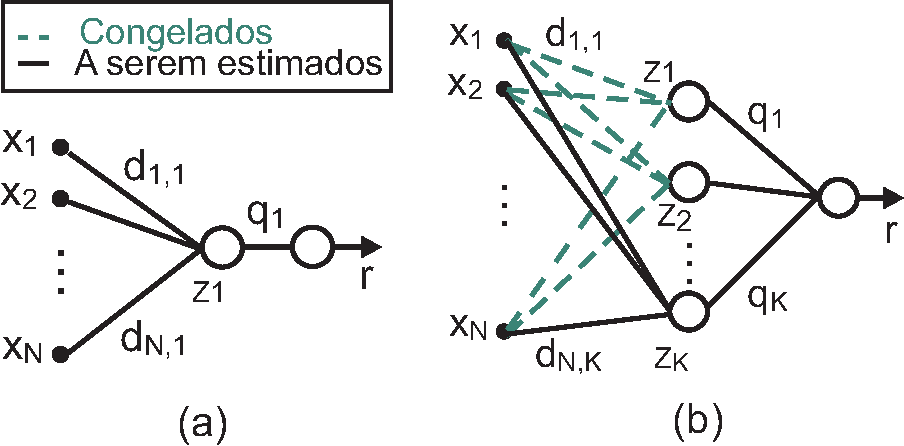
\includegraphics[width=9.5cm]{cap4_pcd}
\caption{Modelos neurais para estimar (a) a primeira e (b) a
k-�sima PCD.} \label{fig_pcd}
\end{figure}

No processo de estima��o, estat�stica de ordem elevada � acessada a partir da utiliza��o de
fun��es de ativa��o n�o-lineares. Considerando que K componentes principais foram estimados, t�m-se:
\begin{equation}\label{ica_eq}
\left[\begin{array}{c}
z_1\\
\vdots \\
z_K
\end{array}\right]=
\underbrace{\left[\begin{array}{c c c}
d_{11} & \dots & d_{1N}\\
\vdots & \ddots & \vdots\\
d_{K1} & \dots & d_{KN}
\end{array}\right]}_{\mathbf{D}} \times
\left[\begin{array}{c}
x_1\\
\vdots \\
x_N
\end{array}\right]
+
\underbrace{\left[\begin{array}{c}
b_{1}\\
\vdots \\
b_K
\end{array}\right]}_{\mathbf{b}},
\end{equation}
\\
ou, na forma matricial: $\mathbf{z}=\mathbf{D}\mathbf{x}+\mathbf{b}$.

Outros modelos que, de modo semelhante a PCD, utilizam redes
neurais para extrair caracter�sticas discriminantes de um conjunto
de sinais foram propostos nos trabalhos~\cite{article:nnfex1:1996,article:nnfex2:1996,article:nnfex:1999}.


\subsection{Utilizando os R�tulos de Classe como Sinais de Entrada para os Algoritmos de ICA}\label{sec_icafex1}

No trabalho \cite{article:icaClasp:2003} foi proposta a utiliza��o
dos r�tulos de classes como entrada para os algoritmos de
estima��o dos componentes independentes. Conforme mostrado na
Figura \ref{fig_icaFex1}, num problema de classifica��o bin�ria
(com apenas duas classes), para cada exemplo de entrada �
associado um novo atributo $c$ com valor igual a 1 (para a classe
1) e -1 (para a classe 2). O bloco G pode ser utilizado para
estimar os modelos linear ou n�o-linear da ICA, a depender do
algoritmo de treinamento utilizado.

\begin{figure}[h]
\centering
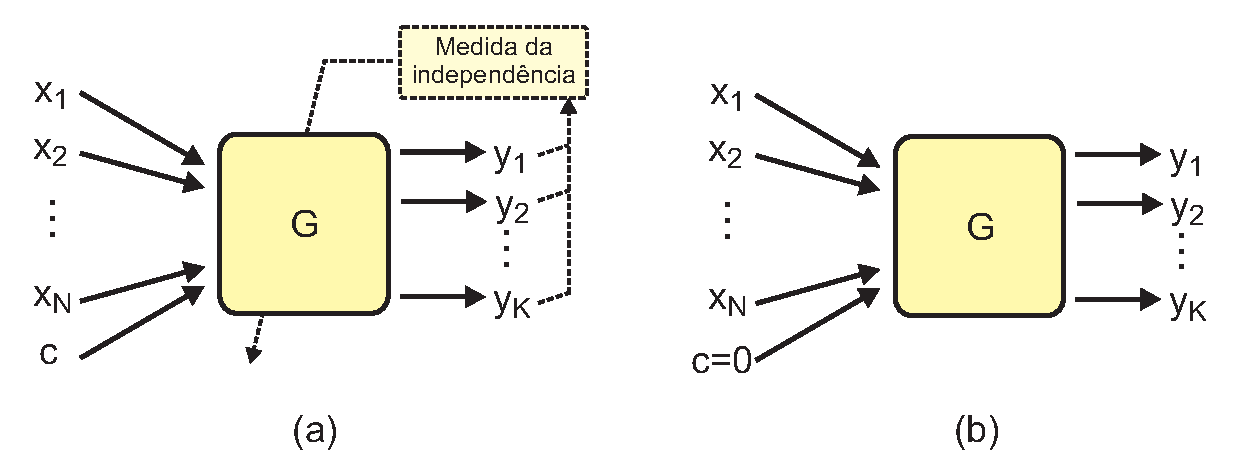
\includegraphics[width=15cm]{ICA_Fex}
\caption{Diagramas de (a) treinamento e (b) opera��o dos
algoritmos de ICA/NLICA utilizando informa��o das classes na
entrada.}\label{fig_icaFex1}
\end{figure}

O par�metro $c$ � adicionado ao vetor de atributos original
$\mathbf{x}=[x_1,x_2,...,x_N]$, gerando
$\mathbf{x}_C=[x_1,x_2,...,x_N,c]$. Para treinamento dos
algoritmos de ICA utiliza-se como entrada o vetor $\mathbf{x}_C$.

Como, num cen�rio pr�tico de opera��o do sistema classificador, os
r�tulos de classe n�o estar�o dispon�veis, a informa��o das
classes deve ser removida dos componentes estimados. Isso pode ser
feito removendo-se as conex�es da entrada $c$ ao modelo, ou
substituindo $c$ por um vetor de zeros.

Em um trabalho semelhante \cite{article:icafexI:2001}, o mesmo
procedimento de treinamento foi adotado, por�m o modelo da ICA
utilizado � linear e quadrado (mesmo n�mero de entradas e sa�das,
n�o havendo portanto redu��o de dimens�o). Ap�s a estima��o dos
componentes, aqueles que tem pesos de baixa amplitude s�o
eliminados, produzindo um conjunto mais compacto de
caracter�sticas discriminantes.

%Um outro modo de utilizar a informa��o das classes no processo de
%estima��o dos componentes independentes foi proposto em
%\cite{article:icafexII:2002}. Neste caso, conforme ilustrado na
%Figura \ref{fig_icaFex2}, os componentes estimados na sa�da devem
%ser independentes e apresentar m�xima informa��o m�tua com os
%r�tulos de classe $c$. A fun��o custo a ser maximizada (este
%trabalho restringe-se ao modelo linear da ICA) � definida como:
%\begin{equation}
% L(\mathbf{W})= - \log|\det \mathbf{W}| + \sum_{i=1}^d H(z_i) - \sum_{i=1}^d I(z_i,c)
%\end{equation}
%onde $\mathbf{W}$ � a matriz da ICA, $z_i$ s�o os componentes
%independentes estimados e $c$ o vetor de r�tulos de classe.
%
%\begin{figure}[h]
%\centering
%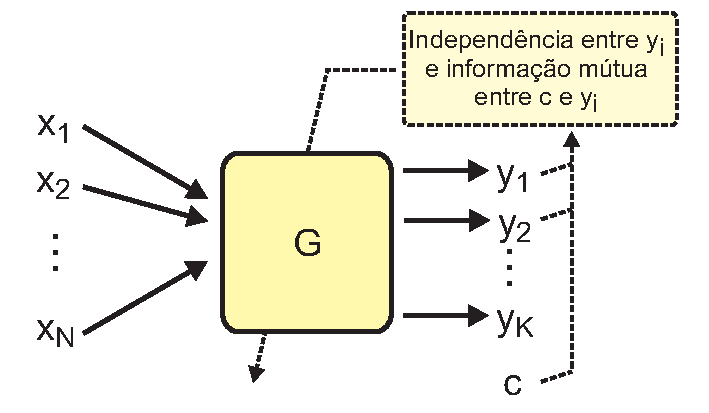
\includegraphics[width=10cm]{ICA_Fex2}
%\caption{Modelo da ICA que utiliza a informa��o das classes em
%conjunto com os componentes estimados na fun��o custo.}
%\label{fig_icaFex2}
%\end{figure}

%\subsection{Componentes Independentes para Cada Classe}\label{sec_icafex12}
%
%Um outro modo de utilizar informa��o supervisionada no contexto da ICA foi
%proposto em~\cite{article:icafexIII:2005} e, no caso de um problema de classifica��o
%em M classes, consiste em realizar a estima��o de M modelos da ICA utilizando, para cada um, apenas amostras da
%classe $m$ (ver Figura \ref{fig_icaFex3}). Pode-se observar que as sa�das de cada bloco
%$G_m$ s�o utilizadas como entradas para um classificador
%especialista na identifica��o da classe $m$. Ao final do
%processamento, um combinador utiliza as informa��es dos $m$
%classificadores para atribuir o r�tulo de classe (produzindo a
%decis�o final).

%\begin{figure}[h]
%\centering
%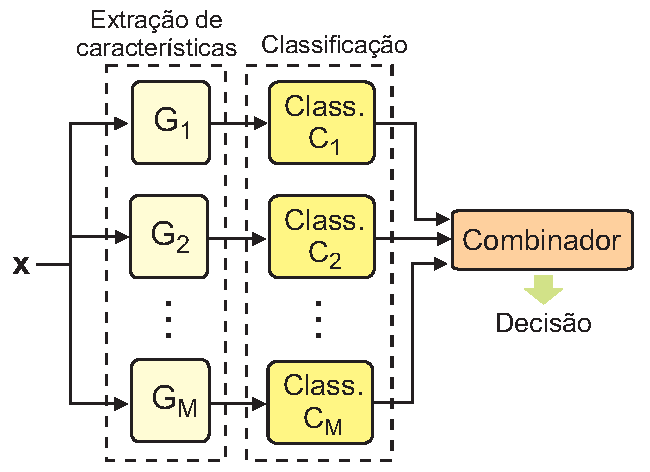
\includegraphics[width=10cm]{ICA_Fex3}
%\caption{Sistema de classifica��o baseado em modelos da ICA
%estimados para cada classe.}\label{fig_icaFex3}
%\end{figure}

%No trabalho \cite{article:icafexIII:2005}, este modelo foi capaz
%de produzir alta efici�ncia no diagn�stico ac�stico de
%equipamentos industriais. A grande vantagem desta abordagem � que
%pode-se utilizar algoritmos tradicionais de ICA/NLICA, sem a
%necessidade de modi\-fica\-��es (o que n�o ocorre para os m�todos
%descritos na se��o~\ref{sec_icafex1}). No trabalho descrito acima
%foi utilizado o algoritmo FastICA para estima��o dos componentes
%independentes.

\subsection{Proposta de Algoritmo para Estima��o de Componentes Independentes e Discriminantes}\label{sec_icafex2}

No desenvolvimento desta tese, foi proposto um m�todo alternativo
para estima��o de componentes independentes e discriminantes. No
trabalho~\cite{article:simas:neucom2010}, foi apresentado um
algoritmo de treinamento para um modelo p�s n�o-linear (PNL)
modificado. Este m�todo ser� descrito a seguir.

Conforme ilustrado na Figura \ref{fig_model_mpnl}, um bloco de
compacta��o foi adicionado ao modelo PNL, com o objetivo de
transformar o conjunto de N atributos em K componentes (com
N$<$K). Assim, a arquitetura proposta � adequada para o caso
sobre-determinado (quando existem mais sinais observados do que
fontes).

\begin{figure}[h]
\centering
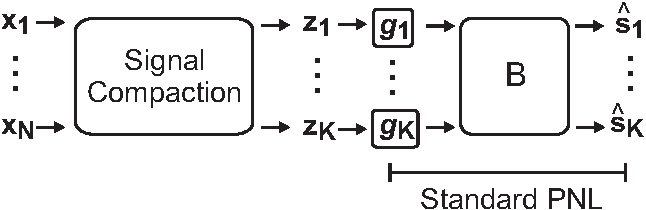
\includegraphics[width=9cm]{mod_pnl}
\caption{Modelo P�s N�o-linear modificado.} \label{fig_model_mpnl}
\end{figure}

O modelo PNL modificado pode ser estimado a partir de dois
procedimentos distintos. Uma abordagem poss�vel � executar a
estima��o do bloco de compacta��o de modo independente do modelo
PNL. Neste caso, a compacta��o se configura numa etapa de
pr�-processamento para a NLICA e pode ser executada, por exemplo
atrav�s da transforma��o PCD.

De modo alternativo, o modelo PNL modificado pode ser estimado
atrav�s do procedimento mostrado na Figura~ \ref{fig_tr_mpnl}, que
combina informa��o de duas fun��es custo diferentes
$c_1(\mathbf{\hat{s}})$, que mede a independ�ncia estat�stica
entre os componentes estimados $\mathbf{\hat{s}}$, e
$c_2(\mathbf{y})$, que avalia a efici�ncia de discrimina��o
produzida a partir de um discriminante linear
(DL)~\cite{book:duda:2000}, onde $\mathbf{y}$ � a sa�da do
classificador.

Considerando um bloco de compacta��o linear, os componentes
independentes estimados s�o descritos por:
\begin{equation}\label{hole_model}
\hat{s}_i=\sum_{j=1}^K b_{ij} g_j(z_j) \hspace{35pt} i=1,...,K
\end{equation}
onde  $\mathbf{z}=\mathbf{D}\mathbf{x}$, $\mathbf{D}$ � uma matriz
retangular (K$\times$N) de compacta��o e os $b_{ij}$ s�o elementos
da matriz quadrada $\mathbf{B}$ (K$\times$K) .

\begin{figure}
\centering
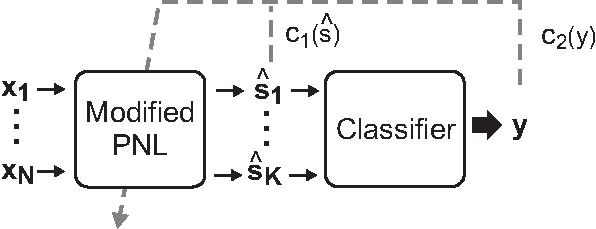
\includegraphics[width=9cm]{treina_mpnl}
\caption{Procedimento de treinamento para o modelo p�s n�o-linear
modificado.} \label{fig_tr_mpnl}
\end{figure}

A estima��o das n�o-linearidades $g_i(.)$ � feita de modo
semelhante ao proposto no trabalho~\cite{article:jutten:1999}, assim, cada fun��o � aproximada por:
\begin{equation}\label{gi}
    g_i (z_i)=  \sum _{h=1}^{N_H} \beta_{hi} \tanh (\omega_{hi} z_i -
    \eta_{hi}) \hspace{35pt} i=1,...,K
\end{equation}
onde $\beta_{hi}$, $\omega_{hi}$ e $\eta_{hi}$ s�o par�metros a
serem determinados.

O objetivo do m�todo proposto � estimar o conjunto de par�metros $\mathbf{D}$,
$\mathbf{B}$, $\beta_{hi}$, $\omega_{hi}$ e $\eta_{hi}$ que
maximiza a fun��o custo definida por:
\begin{equation}\label{eqcf}
    c(\mathbf{\hat{s}},\mathbf{y}) = \frac{\alpha_1}{c_1(\mathbf{\hat{s}})+\alpha_3}+ \alpha_2 \, c_2(\mathbf{y})
\end{equation}
sendo $\alpha_1$, $\alpha_2$ e $\alpha_3$ constantes a serem
previamente escolhidas. � importante observar que o prop�sito de
$\alpha_3$ � limitar o primeiro termo da Equa��o~\ref{eqcf}, quando
$c_1(\mathbf{\hat{s}})\rightarrow 0$. Valores adequados para as
tr�s constantes ser�o indicados a seguir. O n�mero de componentes
independentes a serem estimados (K) precisa ser escolhido a
priori. Na pr�tica, se K for desconhecido, pode-se utilizar um
procedimento semelhante ao descrito na Se��o~\ref{sec_pcd} para a
escolha do n�mero de componentes principais de discrimina��o (PCD).

A fun��o custo que avalia a independ�ncia estat�stica
($c_1(\mathbf{\hat{s}})$) utiliza uma medida do cumulante de
quarta ordem, semelhante � proposta no algoritmo JADE para a
ICA~\cite{article:Cardoso:1993}:
\begin{equation}\label{c1-1}
    c_1(\mathbf{\hat{s}})= \sum_{\substack{i,j=1\\ i<j}}^K \,\,\, \sum_{l,m=1}^K
    \mathbf{cum}\{s_i, s_j, s_l, s_m \}^2
\end{equation}
sendo $\mathbf{cum}\{s_i, s_j, s_l, s_m \}$ o cumulante de quarta
ordem~\cite{book:oja:2001}:
\begin{align}\label{cum}
      \mathbf{cum}\{s_i, s_j, s_l, s_m \}=&E\{s_i, s_j, s_l, s_m \}-E\{s_i, s_j\} E\{s_l, s_m
    \} \nonumber \\
     &- E\{s_i, s_l\} E\{s_j, s_m \} - E\{s_i, s_m \} E\{s_j, s_l \}
\end{align}

Um modo para calcular a medida da independ�ncia baseada no
cumulante de quarta ordem foi proposto
em~\cite{article:cross:2006}, e utilizado neste trabalho para
estimar $c_1(\mathbf{\hat{s}})$. � interessante notar que
$c_1(\mathbf{\hat{s}})$ � uma sempre n�o-negativa e zero para
sinais independentes, ent�o, maximizar a independ�ncia entre os
componentes $\mathbf{\hat{s}}$ implica em minimizar
$c_1(\mathbf{\hat{s}})$.

A fun��o custo que avalia a efici�ncia de discrimina��o � o �ndice
soma-produto (SP) normalizado, que para um problema de
classifica��o em M classes � definido por:
\begin{equation}\label{eq_sp}
    c_2 (\mathbf{y})=\sqrt{\displaystyle{\frac{\sum_{i=1}^M Ef_i}{M}}\times
    \sqrt[M]{\prod_{i=1}^M
    Ef_i}}
\end{equation}
onde $Ef_i$ � a efici�ncia de discrimina��o obtida para a classe
$i$. A fun��o definida na Equa��o~\ref{eq_sp} varia no intervalo
[0,1] e alcan�a o m�ximo quando $Ef_i=1$ para $i=1,...,M$
(efici�ncia total). Uma caracter�stica de $c_2(\mathbf{y})$ � sua
sensibilidade a degrada��o da efici�ncia para qualquer classe.

Considerando que $c_1(\mathbf{\hat{s}}) \geq 0$ e $0\leq
c_2(\mathbf{y})\leq 1$, as constantes $\alpha_i$, na
Equa��o~\ref{eqcf} s�o escolhidas para produzir $0 \leq
c(\mathbf{\hat{s}},\mathbf{y}) \leq 1$. Usando por exemplo,
$\alpha_1=\alpha_3 /2$, $\alpha_2=0.5$ e $\alpha_3=0.001$, o mesmo
fator de pondera��o � dado para os termos de ambos, $c_1$ e $c_2$.

Para a otimiza��o de
$c(\mathbf{\hat{s}},\mathbf{y})$ foi utilizado um algoritmo gen�tico (AG) simples,
conforme mostrado em~\cite{Book:Goldberg:1989,book:haupt:2004}, ao qual foram
adicionados, elitismo, \textit{crossover} uniforme e genoc�dio
peri�dico. Os algoritmo gen�ticos s�o m�todos de busca global capazes de apresentar desempenho
satisfat�rio mesmo em problemas onde a superf�cie de erro � n�o-linear e apresenta �timos locais. Uma outra
caracter�stica do AG � que n�o h� a necessidade do c�lculo do gradiente da fun��o de erro, pois opera
diretamente com o resultado da fun��o custo. Mais detalhes a respeito do AG utilizado s�o mostrados no
Ap�ndice~\ref{apend_GA}.

%  \chapter{Resultados e Discussões}
%  \chapter{Conclusões}

  \backmatter
  %\nocite{*}
  \bibliographystyle{coppe-unsrt}
  \bibliography{edsimas}

  \appendix
 %\chapter{Aspectos Te�ricos das T�cnicas de Extra��o de Caracter�sticas}
\label{apend_fex}

Neste ap�ndice ser�o fornecidos os detalhes da teoria envolvida nos
diversos m�todos de extra��o de caracter�sticas utilizados neste
trabalho.

\section{Mapas Auto-Organiz�veis}

O mapa auto-organiz�vel (SOM - \textit{Self Organizing Map}) � uma
rede neural com treinamento n�o-supervisionado, baseado na
aprendizagem competitiva, que � capaz de realizar uma organiza��o
topol�gica das entradas. O SOM foi proposto por Teuvo Kohonen em
1982 \cite{book:kohonen:2001}, sendo capaz de realizar um
mapeamento n�o-linear dos sinais de um espa�o de entrada cont�nuo de
dimens�o $k$ para um espa�o de caracter�sticas discreto que, em
geral, � bidimensional. Cada neur�nio da grade est� diretamente
conectado a todos os n�s de entrada. Na Figura \ref{soms} pode-se
visualizar o diagrama de um mapa auto-organiz�vel bi-dimensional.

\begin{figure}[h!]
\centering
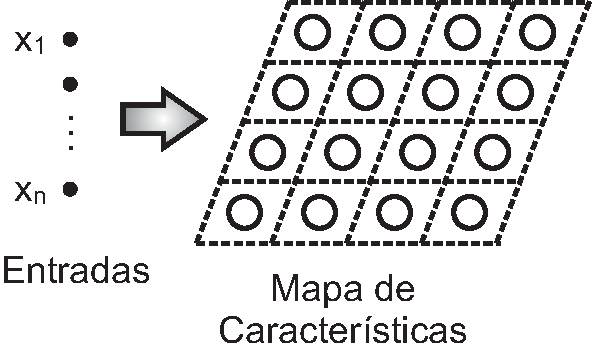
\includegraphics[width=6cm]{cap3_som}
\caption{Diagrama de um mapa auto-organiz�vel} \label{soms}
\end{figure}

O mapa auto-organiz�vel compacta a informa��o e preserva rela��es
topol�gicas ou m�tricas do conjunto de sinais. Os SOM est�o ligados
� ICA por conseguirem extrair informa��es ocultas dos sinais de
forma n�o supervisionada \cite{article:foo:2006}. Uma apro\-xi\-ma��o
das componentes independentes n�o-lineares pode ser obtida
utilizando mapas auto-organiz�veis \cite{book:oja:2001}.

Tr�s processos est�o envolvidos na forma��o do mapa auto-organiz�vel:
a \textbf{competi��o}, onde, para cada vetor de entrada, h� apenas um
neur�nio vencedor; a \textbf{coopera��o}, quando o neur�nio vencedor
determina uma vizinhan�a topol�gica de neur�nios excitados; e a
\textbf{adapta��o}, que procede ao ajuste dos pesos sin�pticos para
refor�ar a resposta do neur�nio vencedor, e de seus vizinhos, ao
padr�o de entrada.

Considerando vetores de entrada $\mathbf{x}=[x_1,x_2,...,x_k]^T$, como os 
neur�nios s�o totalmente conectados �s entradas, o vetor de pesos sin�pticos 
do neur�nio j pode ser definido por: $\mathbf{w}j=[w_{1j},w_{2j},...,w_{kj}]^T$. 
A atualiza��o do vetor de pesos � feita atrav�s da equa��o:
\begin{equation}\label{pesos_som}
    \mathbf{w_j(n+1)}=\mathbf{w}_j(n)+\eta (n) h_{ij}(n)(\mathbf{x}(n)-\mathbf{w}_j(n)),
\end{equation}
\\
sendo $\eta (n)$ a taxa de aprendizagem, um tipo de fun��o de
vizinhan�a $h_{ij}(n)$ usualmente utilizada � definida por:
\begin{equation}\label{neigbor}
h_{ij}(n)=\exp(-d_{ij}^2/2\sigma^2(n))
\end{equation}
\\
onde $d_{ij}$ � a dist�ncia do neur�nio j para o neur�nio vencedor i
e $\sigma(n)$ � a largura da fun��o vizinhan�a na n-�sima itera��o.

%... falar de outras fun��es de vizinhan�a utilizadas ...

O mapa de caracter�sticas possui algumas propriedades, listadas a
seguir \cite{haykin:nn:2008}:

\begin{enumerate}
  \item � formado pelo conjunto de
vetores de pesos sin�pticos $\mathbf{w}_i$ no espa�o de sa�da discreto e
fornece uma boa aproxima��o para o espa�o de entrada;

  \item � ordenado de modo
topol�gico. Padr�es de entrada semelhantes s�o mapeados para regi�es
adjacentes no mapa de caracter�sticas;

  \item regi�es do espa�o de entrada que possuem alta
probabilidade de ocorr�ncia s�o mapeadas para dom�nios maiores do
espa�o de sa�da;

  \item a matriz de pesos sin�pticos pode ser defnida por:
\begin{equation}
  \mathbf{W}=[\mathbf{w}_1,\mathbf{w}_2,...,\mathbf{w}_P],
\end{equation}
onde P � o n�mero de neur�nios do mapa.

\end{enumerate}

No mapa de caracter�sticas, o neur�nio que apresentar maior sa�da �
consi\-derado o vencedor, ou seja a sa�da do SOM � do tipo ``vencedor
leva tudo" (WTA - \textit{winner takes all}). O neur�nio ativado �
escolhido a partir de sua semelhan�a com a entrada $\mathbf{x}_A$ apresentada. �
comum a utiliza��o da dist�ncia euclidiana como m�trica da
proxi\-midade entre dois vetores; nesse caso, o neur�nio vencedor �
aquele que minimiza $i(\mathbf{x})=\| \mathbf{x}_A-\mathbf{w_j}
\|$.

Uma outra forma de operar um mapa auto-organiz�vel � utilizar as proje��es dos sinais de entrada no mapa de
caracter�sticas, ou seja as sa�das $u_j$ de cada neur�nio j que podem ser calculadas por:
\begin{equation}\label{som_out}
 u_j=\mathbf{x}^T\mathbf{w_j}
\end{equation}
O vetor $\mathbf{u}=[u_1,...,u_K]^T$ pode ser considerado como a proje��o de $\mathbf{x}$ no mapa de caracter�sticas.

Os mapas auto-organiz�veis pertencem � classe de algoritmos de
codifica��o vetorial, sendo capazes de encontrar, de forma
otimizada, um n�mero fixo de vetores ou palavras de c�digo que
melhor representem o conjunto de sinais.

\subsection{Quantiza��o Vetorial por Aprendizado}

A quantiza��o vetorial (VQ - \textit{Vector Quantization}) � uma
t�cnica de codifica��o onde um espa�o de entrada � mapeado em um
grupo finito de vetores repre\-sentativos (\textit{codebook})
\cite{article:gersho:1982}. A codifica��o � definida como um
particionamento do espa�o de entrada em um n�mero finito de regi�es.
O quantizador realiza um mapeamento do espa�o $\mathbb{R}^k$, em um
subconjunto finito $Y$ de $\mathbb{R}^k$:

\begin{equation}\label{lv1}
\begin{array}{cc}
  Q: & \mathbb{R}^k \rightarrow \mathbf{Y}
\end{array}
\end{equation}
\\
sendo $ \mathbf{Y}=\{y_1,y_2,...,y_k\}$ o livro de c�digo (\textit{codebook}). Para cada
palavra de c�digo $y_i$ existe uma parti��o $R_i$ do espa�o de
entrada que satisfaz:
\begin{equation}\label{lv2}
R_i=Q^{-1}(\mathbf{y_i})=\{ \mathbf{x} \in  \mathbb{R}^k :
Q(\mathbf{x})=\mathbf{y}_i \}
\end{equation}
\begin{equation}\label{lv3}
    \begin{array}{ccc}
  \bigcup_{i=1}^{N} R_i= \mathbb{R}^k, &  R_i \bigcap R_j=0,&i\neq j
\end{array}
\end{equation}
\\
Quando um quantizador vetorial possui m�nima distor��o � denominado
\textbf{quantizador de Voronoi}. Neste caso, diz-se que o espa�o de
entrada est� particionado de acordo com a regra do vizinho mais
pr�ximo, e as parti��es criadas s�o chamadas de c�lulas de Voronoi
\cite{article:gray:1984}. Usando-se a dist�ncia euclidiana como
par�metro de distor��o, o quantizador $Q^*$ � dito �timo se, para
qualquer outro quantizador $Q$, com o mesmo n�mero de pontos, a
condi��o abaixo � satisfeita:

\begin{equation}\label{llv}
    E|| \mathbf{x} - Q^*(\mathbf{x}) ||^2 \leq E|| \mathbf{x} - Q^(\mathbf{x}) ||^2
\end{equation}
\\
As palavras de c�digo ou os vetores de Voronoi podem ser calculados
de modo aproximado pelo algoritmo SOM. O \textit{codebook} � formado a partir
dos pesos sin�pticos dos neur�nios do mapa. As c�lulas de Voronoi
s�o compostas pelos pontos do espa�o de entrada que est�o mais
pr�ximos do vetor de c�digo correspondente.

Em um problema de classifica��o, pode-se empregar a quantiza��o vetorial por aprendizado (\textit{Learning Vector
Quantization}) \cite{article:kohonenLVQ:1990}, que utiliza informa��es sobre as classes para mover
ligeiramente os vetores de Voronoi, visando a uma melhora no desempenho de decis�o do classificador.

Na sua forma b�sica, o algoritmo LVQ escolhe aleatoriamente um vetor
de entrada $\mathbf{x}$; quando seu r�tulo de classe
$\mathcal{C}_{\mathbf{x_i}}$ e o de um vetor de Voronoi
$\mathbf{w_c}$ concordam, ent�o, $\mathbf{w_c}$ � movido na dire��o
de $\mathbf{x}$:

\begin{equation}\label{lvq1}
  \mathcal{C}_{\mathbf{w_c}}=\mathcal{C}_{\mathbf{x_i}} \rightarrow \mathbf{w_c}(n+1)=\mathbf{w_c}(n)+
    \alpha[\mathbf{x}-\mathbf{w_c}(n)]
\end{equation}
\\
onde $\alpha$ � a taxa de aprendizagem ($0< \alpha <1$). Em caso
contr�rio, $\mathbf{w}$ � afastado de $\mathbf{x}$:

\begin{equation}\label{lvq2}
  \mathcal{C}_{\mathbf{w_c}}\neq \mathcal{C}_{\mathbf{x_i}} \rightarrow
  \mathbf{w_c}(n+1)=\mathbf{w_c}(n)-
    \alpha[\mathbf{x}-\mathbf{w_c}(n)]
\end{equation}
\\
Conforme proposto em \cite{article:kohonenLVQ:1990}, podem ser
implementadas algumas modifica��es na forma b�sica do algoritmo de
LVQ, visando a melhorar o desempenho do m�todo. Chega-se, ent�o, aos
algoritmos LVQ-2 e LVQ-2.1, que ajustam dois vetores de c�digo
simultaneamente.

Alguns exemplos da aplica��o da quantiza��o vetorial por aprendizado
para compress�o de sinais e classifica��o podem ser encontrados em
\cite{article:kohonenLVQ:1990} e \cite{article:dey:1999}.

\subsection{Classifica��o a Partir do Mapa de
Caracter�sticas}\label{mlp_somm}

Considerando um problema de classifica��o, o mapeamento
auto-organiz�vel consegue transformar o conjunto de sinais,
revelando caracter�sticas ocultas. A nova organiza��o do conjunto de
entrada pode ser utilizada para guiar o processo de discrimina��o.
Em \cite{book:freeman:1991} � proposta uma estrat�gia de
classifica��o a partir do mapa de caracter�sticas onde uma rede
neural MLP � conectada �s sa�das do SOM (ver Figura
\ref{som_class}). A MLP � treinada com supervis�o usando informa��es
a respeito das classes de sinais.

\begin{figure}[tbph]
\centering
\includegraphics[width=10cm]{cap3_somclass}
\caption{Diagrama da classifica��o a partir do mapa de
caracter�sticas} \label{som_class}
\end{figure}


\section{An�lise de Componentes Principais}

\section{T�cnicas de Pr�-Processamento - Compacta��o}

No processamento de sinais multi-dimensionais, � comum a utiliza��o de t�cnicas de processamento de sinais
que visam a redu��o da dimensionalidade do problema. O objetivo � projetar os sinais N-dimensionais observados em

\subsection{An�lise de Componentes Principais}

A an�lise de componentes principais (PCA - \textit{Principal
Component Analysis}) � uma t�cnica estat�stica de processamento de
sinais diretamente ligada � transforma��o de \textit{Karhunen-Lo�ve}
\cite{book:pca:2002}. O objetivo da PCA � encontrar uma
transforma��o linear onde os sinais projetados sejam
n�o-correlacionados e grande parcela da energia (vari�ncia) esteja
concentrada num pequeno n�mero de componentes. Para isso, s�o
exploradas informa��es da estat�stica de segunda ordem.

A an�lise de
componentes principais � bastante usada para compacta��o de
informa��o. Como a PCA projeta os sinais em componentes ordenados por energia, uma m�trica geralmente
utilizada para reduzir a dimens�o dos dados consiste na sele��o apenas dos componentes de maior energia,
de modo que o sinal recuperado a
partir da informa��o compactada tenha pequeno erro m�dio quadr�tico
se comparado ao original. A seguir ser�o desenvolvidos, de forma
resumida, os fundamentos matem�ticos da PCA.

Considerando-se um vetor $\mathbf{x}=[x_1,...,x_N]^T$ aleat�rio com $N$ elementos,
assume-se que ele tenha m�dia zero:

\begin{equation}\label{Xm}
    \mathcal{E}\{\mathbf{x}\}=0
\end{equation}
\\
onde $\mathcal{E}\{.\}$ � o operador esperan�a. Se $\mathbf{x}$ tem
m�dia n�o nula faz-se $\mathbf{x}\leftarrow
\mathbf{x}-\mathcal{E}\{\mathbf{x}\}$.

A proje��o $z_i$ de $\mathbf{x}$ na dire��o de $\mathbf{v}_i$ pode
ser expressa por:

\begin{equation}\label{proj1}
    z_i=\mathbf{v}_i^T\mathbf{x}=\sum_{k=1}^N v_{ki}x_k
\end{equation}
\\
Na transforma��o por PCA, os componentes $z_i$ ($i=1,...,N$) devem
ser ortogonais e ordenados (de modo decrescente) pela vari�ncia das
proje��es, sendo, ent�o, $z_1$ a proje��o de m�xima vari�ncia. Para
tornar a vari�ncia independente da norma de $\mathbf{v}_i$, faz-se:

\begin{equation}\label{normaw}
    \mathbf{v}_i \leftarrow \frac{\mathbf{v}_i}{\| \mathbf{v}_i \|}
\end{equation}
\\
Fazendo-se com que $||\mathbf{v}_i||=1$, torna-se a vari�ncia fun��o apenas da dire��o
das proje��es.
%A ortogonalidade garante a n�o-correla��o entre as
%componentes.

Como $\mathcal{E}\{\mathbf{x}\}=0$, ent�o $\mathcal{E}\{z_i\}=0$,
logo a vari�ncia da proje��o $z_i$ � calculada por
$\mathcal{E}\{z_i^2\}$. Seguindo a defini��o da PCA, $z_1$ tem
m�xima vari�ncia; logo, $\mathbf{v}_1$ pode ser encontrado pela maximiza��o
de \cite{book:oja:2001}:

\begin{equation}\label{w1pca}
    J_1^{PCA}(\mathbf{v}_1)=\mathcal{E}\{z_i^2\}=\mathcal{E}\{(\mathbf{v}_1^T\mathbf{x})^2\}
    =\mathbf{v}_1^T\mathcal{E}\{\mathbf{x}\mathbf{x}^T\}\mathbf{v}_1=
    \mathbf{v}_1^T \mathbf{C}_x\mathbf{v}_1,
\end{equation}
\\
onde $\mathbf{C}_x$ � a matriz de covari�ncia de $\mathbf{x}$.

A solu��o para o problema de maximiza��o da equa��o (\ref{w1pca}) pode
ser encontrada na �lgebra linear, em fun��o dos autovetores
$\mathbf{e}_1,\mathbf{e}_2,...,\mathbf{e}_N$ da matriz
$\mathbf{C}_x$. A ordem dos autovetores � tal que os autovalores
associados satisfazem $d_1>d_2>...>d_N$. Desta forma, tem-se:

\begin{equation}\label{pca1}
    \begin{array}{ccc}
      \mathbf{v}_i= \mathbf{e}_i,& & 1\leq i \leq N
    \end{array}
\end{equation}

Percebe-se que a PCA de $\mathbf{x}$ e a decomposi��o por
autovalores da matriz $\mathbf{C}_x$ (de dimens�o $N\times N$) s�o
equivalentes. Limita��es computacionais na extra��o das componentes
principais utilizando as equa��es (\ref{proj1}) e (\ref{pca1})
aparecem quando a dimens�o $N$ do vetor $\mathbf{x}$ aumenta, pois o
processo de obten��o dos autovetores se torna proibitivamente lento.
Nesse caso, uma solu��o � utilizar m�todos iterativos de extra��o
das componentes principais, atrav�s de redes neurais
\cite{article:oja:pca,tese:joao:2007}.


\subsection{Redu��o de Dimens�o}

\begin{figure}[tbph]
\centering
\includegraphics[width=5.5cm]{cap3_pca}
\caption{Compress�o e recupera��o do sinal $\mathbf{x}$ utilizando a
transforma��o por PCA.} \label{pca}
\end{figure}

A principal aplica��o da PCA � a compacta��o da informa��o. A
redu��o de dimens�o � obtida utilizando-se para a reconstru��o do
sinal original $\mathbf{x}$ um n�mero $K$ de componentes principais
sendo $K<N$. Na Figura \ref{pca} � ilustrado o processo de redu��o
de dimens�o utilizando an�lise de componentes principais. Em geral,
o n�mero de componentes � escolhido visando a preservar uma parcela
$V_e$ da energia total, de modo que $\mathbf{\widehat{x}} \approx
\mathbf{x}$. A vari�ncia explicada $V_e$ de um conjunto de
componentes pode ser calculada usando-se:
\begin{equation}\label{vexp}
    V_e(K)=\frac{\displaystyle\sum_{i=1}^K d_i}{\displaystyle\sum_{i=1}^N d_i},
\end{equation}
\\
sendo $d_i$ o autovalor da matriz $\mathbf{C}_x$ de covari�ncia do
processo correspondente � componente $i$.

A transforma��o por PCA � �tima no sentido de representa��o do sinal
nas primeiras componentes, mas n�o h� garantia de que a compacta��o
facilite o processo de classifica��o. Quando as dire��es de maior
vari�ncia coincidem com as de melhor discrimina��o das classes,
ent�o a PCA � tamb�m �til para o reconhecimento de padr�es, em caso
contr�rio, a redu��o de dimens�o pode dificultar a separa��o.
Entretanto, em problemas de classifica��o onde a dimens�o da entrada
� excessivamente grande o pr�-processamento por PCA reduz o custo
computacional e conseq�entemente o tempo de processamento.


\section{An�lise de Componentes Independentes}

\subsection{Princ�pios de Estima��o dos Componentes Independentes}

No modelo b�sico da ICA (ver equa��o (\ref{icamatrix}))assume-se que
a matriz $\mathbf{A}$ � quadrada e n�o s�o considerados os atrasos
temporais nem a exist�ncia de ru�do aditivo. O princ�pio b�sico para
a extra��o das componentes independentes � obtido do teorema do
limite central. Como a soma de duas vari�veis aleat�rias
independentes � sempre mais pr�xima de uma distribui��o normal do
que as vari�veis originais, os sinais misturados $x_i$, que s�o
gerados a partir do somat�rio ponderado das fontes $s_i$, t�m
distribui��es de probabilidade mais semelhantes � Gaussiana quando
comparadas aos sinais originais. As fontes podem ser obtidas ent�o
pela maximiza��o da n�o-Gaussianidade.
%A curtose e a negentropia s�o usualmente
%utilizadas para medi��o da n�o-gaussianidade em ICA.

\subsubsection{Maximiza��o da n�o-Gaussianidade}

A \textbf{curtose} � o cumulante de quarta ordem, e para uma
vari�vel $y$ de m�dia zero e vari�ncia unit�ria � definida por
\cite{book:peebles:2001}:
\begin{equation}\label{curtose}
    kurt(y)=\mathcal{E}\{y^4\}-3(\mathcal{E}\{y^2\})^2.
\end{equation}

Variando no intervalo $[-2,\infty)$, a curtose � igual a zero para
uma vari�vel Gaussiana, os valores negativos indicam
sub-Gaussianidade e os positivos super-Gaussianidade.
%Nas Figuras
%\ref{subgauss} e \ref{supergauss} pode-se visualizar exemplos dos 3
%tipo de distribui��es, gaussiana ou normal, sub-gaussiana (mais
%achatada) ou super-gaussiana (mais concentrada em torno da m�dia). O
%menor valor da curtose ocorre para vari�veis uniformemente
%distribu�das.
%
%\begin{figure}[tbph]
%\begin{center}
%\subfigure[]{\label{subgauss}\epsfig{file=cap3_subgauss,width=11cm,clip=}}
%\subfigure[]{\label{supergauss}\epsfig{file=cap3_supergauss,width=11cm,clip=}}
%\end{center}
%\caption{Distribui��es de probabilidade (a) sub-gaussiana e (b)
%super-gaussiana.}
%\end{figure}

A curtose � um par�metro estat�stico facilmente calculado a partir
das rea\-liza��es da vari�vel aleat�ria, por�m seu valor pode ser
bastante influenciado por um pequeno conjunto de pontos na cauda da
distribui��o \cite{book:spiegel:stat}, sendo, nesse caso, pouco
robusta para a estimativa da n�o-Gaussianidade. Conhecidos como
intrusos (ou \textit{outliers}) esses pontos podem realmente
pertencer � vari�vel aleat�ria, ou ter sido artificialmente
introduzidos por algum fen�meno desconhecido, como erro de medida ou
de digita��o.

Uma estima��o alternativa da n�o-Gaussianidade pode ser obtida a
partir da \textbf{negentropia}, que � calculada por
\cite{book:cover:1991}:
\begin{equation}\label{negen}
    J(y)=H(y_{gauss})-H(y),
\end{equation}
\\
onde $H(.)$ � a entropia, e $y_{gauss}$ � uma vari�vel aleat�ria
Gaussiana com a mesma m�dia e vari�ncia de $y$. A entropia � um dos
conceitos b�sicos da teoria da informa��o e pode ser interpretada
como o grau de informa��o contido em uma vari�vel. Para uma vari�vel
aleat�ria discreta a entropia � definida como
\cite{article:shannon:1948}:
\begin{equation}\label{entro1}
    H(Y)=-\sum_i P(Y=a_i)log P(Y=a_i),
\end{equation}
\\
onde os $a_i$ s�o os poss�veis valores da vari�vel $Y$, e $P(Y=a_i)$
� a probabilidade de $Y$ ser igual a $a_i$.

Um resultado importante obtido a partir da teoria da informa��o �
que uma vari�vel Gaussiana tem a m�xima entropia entre todas as
vari�veis de mesma vari�ncia. Considerando a equa��o (\ref{negen}),
a negentropia � sempre n�o negativa e zero quando a vari�vel �
Gaussiana, servindo como uma medi��o da n�o-Gaussianidade. O grande
problema no c�lculo de $J(.)$ � a necessidade de se estimar as
probabilidades da equa��o (\ref{entro1}). Para evitar esse c�lculo,
utilizam-se aproxima��es da negentropia. Conforme descrito em
\cite{book:oja:2001}, existem duas aproxima��es mais utilizadas para
a negentropia, uma faz uso de cumulantes de ordem superior:
\begin{equation}\label{eq_neg1}
    J(Y)\approx \frac{1}{12}E\{Y^3\}^2+\frac{1}{48}kurt(Y)^2,
\end{equation}
e outra utiliza fun��es n�o-polinomiais
\cite{article:hyvarinen:1998}:
\begin{equation}\label{eq_neg2}
    J(Y)\approx [k_1 (E\{G_1(Y)\})^2 +
    k_2(E\{G_2(Y)\}-E\{G_2(\nu)\})^2],
\end{equation}
onde $\nu$ � uma vari�vel aleat�ria Gaussiana de m�dia zero e
vari�ncia unit�ria. As fun��es n�o-lineares recomendadas em
\cite{article:hyvarinen:1998} s�o $G_1(y)=y\exp(-y^2/2)$ e
$G_2(y)=|y|$ ou $G_2(y)=\exp(-y^2/2)$.

O uso de cumulantes traz de volta o problema da pouca robustez a
\textit{outliers}. � mostrado em \cite{article:hyvarinen:1998} que o
uso das fun��es n�o-polinomiais leva ao m�todo da m�xima entropia
\cite{book:oja:2001}.

\subsubsection{Minimiza��o da Informa��o M�tua}

Um outro m�todo de estima��o de ICA, tamb�m derivado da teoria da
informa��o, � obtido pela minimiza��o da informa��o m�tua. A
informa��o m�tua $I(.)$ entre $m$ vari�veis aleat�rias escalares
$y_i$ � definida como \cite{article:hyvarinen:2000}:
\begin{equation}\label{mutinf}
    I(y_1,y_2,...,y_m)=\sum_{i=1}^m H(y_i) - H(\mathbf{y})
\end{equation}

A entropia $H(y_i)$ pode ser interpretada como o comprimento de
c�digo (ou a quantidade de informa��o) neces\-s�rio para representar a vari�vel $y_i$. Conforme a
equa��o (\ref{mutinf}), a informa��o m�tua � a diferen�a entre o
somat�rio das entropias de cada uma das $m$ vari�veis $y_i$ e a
entropia do vetor aleat�rio $\mathbf{y}=[y_1,y_2,...y_m]$. Pode-se
provar que a codifica��o mais eficiente � obtida quando se utiliza o
conjunto de vari�veis $\mathbf{y}$. Utilizar as vari�veis
isoladamente sempre gera um maior c�digo, menos quando as $y_i$ s�o
independentes, pois desta forma uma vari�vel n�o carrega informa��o
sobre as demais, sendo a informa��o m�tua igual a zero. Desta
forma, $I(y_1,y_2,...,y_m)$ pode ser utilizada como uma medida da
depend�ncia entre as vari�veis. A matriz $\mathbf{W}$ de
transforma��o inversa da ICA, conforme equa��o \ref{icamatrix2}, pode
ser estimada atrav�s da minimiza��o da informa��o m�tua dos sinais
$s_i$ recuperados.

\subsubsection{ICA atrav�s da Descorrela��o N�o-Linear}

A igualdade da equa��o:
\begin{equation}\label{indep22}
    \mathcal{E}\{g(x)h(y)\}=\mathcal{E}\{g(x)\}\mathcal{E}\{h(y)\}
\end{equation}
\\
repetida aqui para comodidade
do leitor, garante que as vari�veis $x$ e $y$ s�o independentes quando todas
fun��es $g(.)$ e $h(.)$,integr�veis em $x$ e $y$ s�o
descorrelacionadas. Portanto, a extra��o das ICs pode ser obtida
testando-se a correla��o entre todas as fun��es n�o-lineares $g(.)$ e
$h(.)$.

Existem alguns algoritmos propostos na literatura para o problema da
decorrela��o n�o-linear, como o \textit{H�rault-Jutten}
\cite{book:oja:2001} e o \textit{Chichocki-Unbehauen}
\cite{article:Cichocki:1996}, mas como n�o � poss�vel testar a
descorrela��o entre todas as fun��es n�o-lineares, escolhem-se $f(.)$
e $g(.)$ visando-se a obter boas aproxima��es das componentes
independentes. O algoritmo \textit{H�rault-Jutten}, por exemplo,
aconselha o uso de $f(y)=y^3$ e $g(y)=arctg(y)$, j� o
\textit{Chichocki-Unbehauen} sugere uma fun��o polinomial e a
tangente hiperb�lica.

A PCA n�o-linear (NLPCA - \textit{Non-linear Principal Component
Analysis}) pode ser vista como uma extens�o n�o linear da PCA, e �
capaz de encontrar proje��es descorrelacionadas n�o-linearmente.
Enquanto o objetivo da PCA � minimizar o erro m�dio quadr�tico de
reconstru��o do sinal projetando as componentes numa base
ortonormal, a NLPCA pode ser definida de modo simples atrav�s da
fun��o-objetivo a ser minimizada:
\begin{equation}\label{nlpca}
    J(\mathbf{w}_1,\mathbf{w}_2,...,\mathbf{w}_n)=\mathcal{E}\{||\mathbf{x}-\sum_{i=1}^n g_i(\mathbf{w}_i^Tx)\mathbf{w}_i||^2\},
\end{equation}
\\
onde $g_1(.), g_2(.), ..., g_n(.)$ � um conjunto de fun��es
escalares e n�o-lineares, e os vetores $\mathbf{w}_i$ formam a base
do sub-espa�o onde ser�o projetadas as entradas $\mathbf{x}$. Quando
o m�nimo de $J(\mathbf{w}_1,\mathbf{w}_2,...,\mathbf{w}_n)$ for
encontrado, o produto $\mathbf{w}_i^Tx$ dar� as componentes
principais n�o-lineares. Se $g_i(y)=y$ para todo $i$, ent�o equa��o
(\ref{nlpca}) se reduz � fun��o objetivo da PCA. Quando os sinais
satisfazem ao modelo da ICA, mostrado na equa��o (\ref{icamatrix}), a
NLPCA obt�m uma aproxima��o das componentes independentes.


\subsection{Pr�-Processamento dos Sinais para ICA}

Em geral, os algoritmos de extra��o das componentes independentes
t�m seu trabalho simplificado quando os sinais s�o centralizados, ou
seja, t�m sua m�dia removida fazendo-se:
\begin{equation}\label{remedia}
    \mathbf{x}\leftarrow \mathbf{x}-\mathcal{E}\{\mathbf{x}\}
\end{equation}

Outra transforma��o importante � o branqueamento. Um vetor
$\mathbf{z}=(z_1,z_2,...,z_n)^T$ � dito branco quando os elementos
$z_i$ s�o descorrelacionados e t�m vari�ncia unit�ria. O
branqueamento pode ser realizado por uma transforma��o linear:
\begin{equation}\label{branq}
    \mathbf{z}=\mathbf{V}\mathbf{x}
\end{equation}

O branqueamento, que � apenas a descorrela��o seguida de uma
norma\-liza��o, pode ser realizado por uma transforma��o atrav�s de
PCA. Com as vari�veis branqueadas a extra��o da ICA � facilitada,
pois os sinais j� est�o descorrelacionados.

Em problemas com vetores de entrada de alta dimens�o, � importante
a compacta��o da informa��o atrav�s de PCA ou An�lise de Relev�ncia
para facilitar o processo de extra��o das componentes independentes.

\subsection{Principais Algoritmos para ICA}

Diversos algoritmos v�m sendo propostos para a extra��o das
componentes independentes. Essas rotinas diferem basicamente no
princ�pio te�rico no qual fundamentam a obten��o das componentes
independentes (n�o-Gaussianidade, informa��o m�tua, descorrela��o
n�o-linear, etc) e na forma fazem a otimiza��o da fun��o objetivo
escolhida. Os principais par�metros para avalia��o de desempenho s�o
o tempo de processamento (complexidade computacional) e a precis�o
na extra��o das componentes.

Um estudo comparativo entre diversos m�todos de estima��o das
componentes independentes foi realizado em \cite{book:oja:2001}. O
algoritmo \textbf{FastICA}, descrito com detalhes em
\cite{book:oja:2001} e \cite{article:hyvarinen:2000}, � o que
apresenta menor custo computacional. Algoritmos que realizam
descorrela��o n�o linear e NLPCA t�m desempenho semelhante ao
FastICA em termos da precis�o na obten��o da matriz $\mathbf{W}$,
por�m exigem maior esfor�o de computa��o. O algoritmo \textbf{JADE}
(\textit{Joint Approximate Diagonalization of Eigen-matrices})
proposto em \cite{article:Cardoso:1993} tamb�m � muito utilizado em
ICA, mostrando bons resultados.

\subsubsection{Algoritmo FastICA}

Considerando as aproxima��es da negentropia mostradas nas Equa��es
(\ref{eq_neg1}) e (\ref{eq_neg2}), e o fato de que a minimiza��o da
negentropia leva � independ�ncia estat�stica, no trabalho
\cite{article:fastica:1999} foram propostos algoritmos de ponto fixo
para ICA (chamados FastICA), que utilizam itera��es semelhantes �s
de Newton \cite{Book:Luenberger:1984}. Entre as vantagens deste
algoritmo pode-se citar simplicidade computacional, baixa utiliza��o
de mem�ria e boas caracter�sticas de converg�ncia
\cite{article:hyvarinen:2000}.

A partir de algumas manipula��es da equa��o (\ref{eq_neg2}), o
algoritmo FastICA para estima��o de uma componente independente �
formulado a seguir para sinais pr�-branqueados:
\begin{enumerate}
  \item Escolha um vetor de pesos inicial $\mathbf{w}$ de modo aleat�rio;
  \item Fa�a $\mathbf{w}^{+}=E\{\mathbf{x}
  g(\mathbf{w}^T\mathbf{x})\}-E\{g'(\mathbf{w}^T\mathbf{x})\}\mathbf{w}$;
  \item $\mathbf{w}=\mathbf{w}^{+}/\parallel \mathbf{w}^{+}
  \parallel$;
  \item Se o algoritmo n�o tiver convergido voltar para o passo 2.
\end{enumerate}

Os autores sugerem o uso de uma das fun��es g(.) a seguir:
\begin{eqnarray}
% \nonumber to remove numbering (before each equation)
  g_1(x) = \text{tgh}(a_1 x), \\
  g_2(x) = x \exp(-a_2 u^2/2), \\
  g_3(x) = x^3,
\end{eqnarray}
onde $1\leq a_1 \leq 2$ e $a_2 \approx 1$. A escolha da fun��o
n�o-linear pode ser guiada pelas caracter�sticas a seguir
\cite{article:fastica:1999}: a fun��o $g_1(.)$ � indicada quando n�o
h� informa��o a respeito da estat�stica das componentes
independentes, pois o algoritmo apresenta resultados satisfat�rios
para qualquer tipo de distribui��o; o uso de $g_2(.)$ � indicado
quando as componentes independentes s�o super-Gaussianas e o
$g_3(.)$ deve ser utilizada para estimar componentes sub-Gaussianas.

Para estimar mais de uma componente independente pode-se utilizar
m�todos de ortogonaliza��o deflacion�ria como o de Gram-Schimidt
\cite{book:oja:2001}.

\subsubsection{Algoritmo JADE}

No algoritmo JADE (\textit{Joint Approximate Diagonalization of
Eigenmatrices}), as informa��es estat�sticas de segunda e quarta
ordem s�o utilizadas a partir de uma abordagem tensorial. Tensores
\cite{book:tensor:2008} s�o generaliza��es de alta-dimens�o das
matrizes. O tensor cumulante de quarta ordem $\mathbf{T_4}$ � uma
``matriz" de quatro dimens�es onde cada elemento � definido por
$q_{ijkl}=\text{cum}(x_i,x_j,x_k,x_l)$, os �ndices i,j,k e l variam
de 1 at� N (onde N � o n�mero de sinais) e
$\text{cum}(x_i,x_j,x_k,x_l)$ � o cumulante de quarta ordem:
\begin{equation}\label{cum4}
\begin{split}
cum(x_i,x_j,x_k,x_l)=E\{x_i,x_j,x_k,x_l\}
  -E\{x_i,x_j\}E\{x_k,x_l\} \\ -E\{x_i,x_k\}E\{x_j,x_l\}
  -E\{x_k,x_j\}E\{x_i,x_l\}
\end{split}
\end{equation}

Sabe-se que a diagona\-li\-za��o da matriz de correla��o
($\mathbf{C_y}$) produz a descorrela��o entre os componentes de
$\mathbf{y}$ \cite{book:oja:2001}. Para sinais independentes, apenas
quando i=k=j=l os cumulantes de quarta-ordem s�o diferentes de zero.
Considerando isso, os m�todos Tensoriais de ICA prop�e a
diagonaliza��o de $\mathbf{T_4}$ para alcan�ar a independ�ncia
estat�stica \cite{article:Cardoso:1993}.

Embora teoricamente simples, a utiliza��o de m�todos tensoriais de
ICA exigem uma grande quantidade de recursos computacionais para a
decomposi��o em auto-valores de matrizes de quarta-ordem. O
algoritmo JADE prop�e um m�todo aproximado para a diagonaliza��o de
$\mathbf{T_4}$, se tornando mais leve computacionalmente.

Considerando que os dados satisfazem o modelo da ICA para dados pr�-branqueados, pode-se escrever:
\begin{equation}\label{eq_jade0}
    \mathbf{z}=\mathbf{VAs}=\mathbf{W}^T\mathbf{s}
\end{equation}
onde $\mathbf{x=As}$ s�o os sinais observados, $\mathbf{V}$ � a
matriz de branqueamento e $\mathbf{W}^T=VA$ � a matriz de misturas
branqueada. Neste caso, pode-se provar (ver \cite{book:oja:2001} que
o tensor cumulante de $\mathbf{z}$ tem uma estrutura especial e suas
auto-matrizes s�o descritas por:
\begin{equation}\label{eq_jade01}
    \mathbf{M}=\mathbf{w_m w_m}^T
\end{equation}
onde m=1,...,N e $w_n$ s�o as colunas da matriz $\mathbf{W}^T$

O algoritmo JADE utiliza a transforma��o linear $F_{ij}$ da matriz $\mathbf{M}$ definida por:
\begin{equation}\label{jade1}
    F_{i,j}(\mathbf{M})=\sum m_{kl} \text{cum}(x_i,x_j,x_k,x_l)
\end{equation}
onde $m_{kl}$ � um elemento da matriz $\mathbf{M}$.

A decomposi��o em autovalores � vista como um processo de
diagonaliza��o, ent�o busca-se a matriz $\mathbf{W}$ que diagonaliza
$F(\mathbf{M})$ para qualquer $\mathbf{M}$ (ou seja, \linebreak
$Q=\mathbf{W}F(\mathbf{M_i})\mathbf{W}^T$ � uma matriz diagonal).

A fun��o custo do m�todo JADE busca a diagonaliza��o de $\mathbf{Q}$
pela maximiza��o da soma dos elementos de sua diagonal. As matrizes
$\mathbf{M_i}$ utilizadas s�o as automatrizes do tensor cumulante
dos dados, pois assim tem-se um conjunto de N matrizes que cont�m
toda a informa��o relevante a respeito dos cumulantes.

Os m�todos tensoriais \cite{article:fobi:1989,article:Cardoso:1993}
foram, provavelmente, a primeira classe de algoritmos capazes de
executar a ICA de modo realmente eficiente \cite{book:oja:2001}.
Atualmente, estes m�todos s�o mais utilizados para sinais de baixa
dimens�o, pois o custo computacional aumenta rapidamente com o
n�mero de componentes a serem estimados.



\subsubsection{Algoritmo Multiplicativo com Itera��o de Newton}

Um algoritmo multiplicativo para ICA foi proposto por Akuzawa e
Murata em \cite{article:akuzawa:2001}. Usando a curtose como fun��o
para avaliar a independ�ncia, esse algoritmo utiliza estrat�gia de
otimiza��o de segunda ordem, atrav�s do m�todo de Newton
\cite{Book:Luenberger:1984}, para estimar as componentes
independentes.

O algoritmo proposto por Akuzawa n�o requer pr�-branqueamento,
operando diretamente sobre os dados medidos. Resultados
experimentais obtidos em
\cite{article:extakuzawa:2000,article:cuenca:2003} indicam que o
algoritmo de Akuzawa apresenta melhor desempenho que FastICA e JADE
quando os sinais est�o contaminados por ru�do Gaussiano.

Considerando a transforma��o linear $\mathbf{Y}=\mathbf{CX}$, o
objetivo do algoritmo de Akuzawa � encontrar a matriz $\mathbf{C}$
que maximiza a independ�ncia entre as componentes de $\mathbf{y}$.
Os passos a seguir s�o executados durante as itera��es:

\begin{enumerate}
\item Escolher $C_0$ (a matriz de separa��o inicial) e a matriz $\Delta_0$ (N $\times$ N);
\item Calcular a itera��o $C_t=\exp (\Delta_t -1)C_{t-1}$;
\item Avalie a fun��o custo em $C_t$ usando uma expans�o de segunda ordem em torno de $C_{t-1}$;
\item $\Delta_t$ � escolhido como o ponto de sela da fun��o custo;
\item Retorne para o passo 2 at� convergir.
\end{enumerate}

Mais detalhes a respeito da execu��o do passo 4 podem ser
encontradas em \cite{article:akuzawa:2001}. Modifica��es no m�todo
de Akuzawa foram propostos em \cite{article:extakuzawa:2000} com o
objetivo de reduzir o custo computacional pela substitui��o das
itera��es de Newton pelo m�todo quasi-Newton
\cite{Book:Luenberger:1984}.

Comparado com FastICA e JADE, o algoritmo multiplicativo de Akuzawa
� mais lento (mesmo em sua vers�o modificada que utiliza o m�todo de
otimiza��o quasi-Newton), suas vantagens aparecem quando o n�vel de
ru�do aumenta, neste caso o m�todo de Akuzawa apresenta melhores
resultados.

\section{ICA N�o-Linear}

Conforme mostrado no Cap�tulo \ref{cap_ica}, o modelo da ICA
n�o-linear (NLICA) apresenta uma formula��o mais geral que o linear.
A seguir ser� mostrado o desenvolvimento te�rico de um algoritmo
para a estima��o das componentes independentes no modelo p�s
n�o-linear.

\subsection{Algoritmo Taleb-Jutten para o Modelo PNL}

Um dos primeiros algoritmos para o modelo p�s n�o-linear da ICA foi
proposto por Taleb e Jutten no trabalho \cite{article:jutten:1999}.
Este algoritmo � robusto a varia��es na distribui��o de
probabilidade das fontes, pois executa estima��o iterativa da
estat�stica das componentes independentes estimadas atrav�s do
c�lculo da fun��o escore:
\begin{equation}\label{juttenpnl1}
    \psi = p'_{Yi}(u) / p_{Yi}(u),
\end{equation}
conforme Figura \ref{fig_pnljutten}.

Cada fun��o n�o-linear $g_k$ (k=1,...,N) � modelado por redes MLP
com um neur�nio linear na sa�da:
\begin{equation}\label{juttenpnl2}
    g_k (u)=\sum_{h=1}^{N_H} \xi^{h} \sigma (\omega^h u - \eta^h),
\end{equation}
onde $N_H$ � o n�mero de neur�nios ocultos. A diverg�ncia de
Kullback-Lieber � utilizada para encontrar as regras de aprendizado
para a estima��o das fun��es n�o-lineares
\cite{article:jutten:1999}.

\begin{figure}[h!]
\centering
\includegraphics[width=6.5cm]{cap3_pnljutten}
\caption{Diagrama do algoritmo de Taleb-Jutten para o modelo PNL.}
\label{fig_pnljutten}
\end{figure}

Como existem v�rios par�metros a serem ajustados no modelo inverso
proposto e a otimiza��o envolve fun��es n�o-lineares, o algoritmo
pode apresentar problemas de converg�ncia para m�nimos locais
\cite{jutten:nlica:2003}. Diferentes procedimentos foram propostos
na literatura para melhorar a efici�ncia de estima��o em modelos
PNL. Em \cite{article:nlica_ga:2001,article:kai:2006} um algoritmo
gen�tico \cite{Book:Goldberg:1989} foi utilizado para executar uma
busca global, evitando o problema dos m�nimos locais. O problema com
esta abordagem � o aumento do custo computacional.

Redes neurais com arquiteturas alternativas tamb�m foram aplicadas
com sucesso na separa��o de misturas PNL. Por exemplo, em
\cite{article:tan:20000} fun��es de base radial (RBF -
\textit{Radial Basis Function}). Em um outro trabalho
\cite{article:solazzi:pnl:2004}, a separa��o foi realizada por redes
neurais com fun��es de ativa��o do tipo \textit{spline}.

 % \chapter{Conceitos Fundamentais em Classifica��o de Sinais}
\label{apend_clas}

A seguir ser�o mostrados os fundamentos te�ricos de algumas t�cnicas
de classifica��o de padr�es, iniciando-se com uma vis�o geral do
problema de decis�o bin�ria. Ser�o apresentadas t�cnicas lineares,
como Filtros Casados e An�lise de Discriminantes, e n�o-lineares,
como Redes Neurais.

\section{Teste de Hip�teses}

Considerando-se inicialmente a discrimina��o entre duas hip�teses
$H_1$ e $H_0$, o problema de classifica��o pode ser resumido pelo
esquema da Figura \ref{class}. A fonte gera as sa�das, que, ap�s
passarem por um meio probabil�stico, precisam ser detectadas a
partir das observa��es do processo. As regras de decis�o, que formam
o sistema classificador, s�o projetadas para maximizar a
probabilidade de detec��o correta.

\begin{figure} \centering
\includegraphics[width=12cm]{cap3_transicao}
\caption{Esquem�tico do problema de classifica��o bin�rio.}
\label{class}
\end{figure}

No caso da decis�o bin�ria, cada vez que uma observa��o � efetuada 4
situa��es podem ocorrer:
\\decidir pela hip�tese $H_1$, sendo $H_0$ verdadeira;
\\decidir pela hip�tese $H_0$, sendo $H_1$ verdadeira;
\\decidir pela hip�tese $H_1$, sendo $H_1$ verdadeira; \\decidir pela hip�tese $H_0$, sendo $H_0$ verdadeira.

%\begin{itemize}
%  \item decidir por $H_1$, sendo $H_0$;
%  \item decidir por $H_0$, sendo $H_1$;
%  \item decidir por $H_1$, sendo $H_1$;
%  \item decidir por $H_0$, sendo $H_0$.
%\end{itemize}
As duas primeiras s�o erros de decis�o, e as duas �ltimas
classifica��es corretas. Cada uma das hip�teses � associada a uma
sa�da da fonte, que � mapeada em uma regi�o do espa�o de observa��o.
Considerando um espa�o de observa��o de dimens�o $N$ finita, um
ponto neste espa�o pode ser representado por um vetor:

\begin{equation}\label{r}
    \mathbf{r}=[r_1,r_2,...,r_N].
\end{equation}
\\
O mecanismo de transi��o probabil�stica gera pontos de acordo com as
densidades de probabilidade condicionais
$P_{\mathbf{r}/H_0}(\mathbf{R}/H_0)$ e
$P_{\mathbf{r}/H_1}(\mathbf{R}/H_1)$. Quando essas probabilidades
s�o conhecidas ou podem ser estimadas de alguma forma, o projeto do
sistema classificador pode ser simplificado. Os crit�rios de
\textit{Bayes} e \textit{Neyman-Pearson} s�o procedimentos cl�ssicos
utilizados para a escolha da regra de decis�o.

\section{Crit�rio de Bayes}

O crit�rio de \textit{Bayes} necessita do conhecimento das
probabilidades a priori $P_1$ e $P_0$ de a fonte produzir $H_1$ ou
$H_0$, das probabilidades condicionais
$P_{\mathbf{r}/H_0}(\mathbf{R}/H_0)$ e
$P_{\mathbf{r}/H_1}(\mathbf{R}/H_1)$ e dos custos $C_{ij}$
associados � escolha da hip�tese $i$ sendo $j$ a verdadeira. O risco
�, ent�o, definido como \cite{book:vantrees1:2001}:
\begin{equation}\label{riscobayes}
    \begin{array}{c}
       \mathfrak{R}=C_{00}P_0\int_{Z_0}P_{\mathbf{r}/H_0}(\mathbf{R}/H_0)d\mathbf{R}
    \\+C_{10}P_0\int_{Z_1}P_{\mathbf{r}/H_0}(\mathbf{R}/H_0)d\mathbf{R}\\
        +C_{11}P_1\int_{Z_1}P_{\mathbf{r}/H_1}(\mathbf{R}/H_1)d\mathbf{R}\\
    +C_{01}P_1\int_{Z_0}P_{\mathbf{r}/H_1}(\mathbf{R}/H_1)d\mathbf{R},
    \end{array}
\end{equation}
\\
onde os elementos do espa�o de observa��o que pertencem �s parti��es
$Z_0$ e $Z_1$ s�o associados, respectivamente, a $H_0$ e $H_1$. As
vari�veis $C_{ij}$ representam o custo da escolha da hip�tese $i$
quando a hip�tese verdadeira � a $j$. Em geral assume-se que o custo
de uma decis�o errada ($C_{ij}$ sendo $i\neq j$) � maior do que o de
um acerto ($C_{ij}$ sendo $i=j$).

Minimizando o risco $\mathfrak{R}$ da equa��o (\ref{riscobayes})
chega-se a \cite{book:vantrees1:2001}:

\begin{equation}\label{seme1}
    \frac{P_{\mathbf{r}/H_1}(\mathbf{R}/H_1)}{P_{\mathbf{r}/H_0}(\mathbf{R}/H_0)}\gtrless_{H_0}^{H_1}\frac{P_0(C_{10}-C_{00})}{P_1(C_{01}-C_{11})};
\end{equation}
\\
a express�o � esquerda � chamada raz�o de verosimilhan�a
($\Lambda(\mathbf{R})$) e a fra��o � direita � o valor limiar
(patamar) do teste ($\kappa$). Com isso, a equa��o (\ref{seme1}) se
reduz a:
\begin{equation}\label{seme2}
  \Lambda(\mathbf{R})  \gtrless_{H_0}^{H_1} \kappa;
\end{equation}
\\
ent�o, se a raz�o de verosimilhan�a � maior que o patamar, decide-se por
$H_1$, em caso contr�rio, escolhe-se $H_0$.

Quando os custos n�o s�o conhecidos, pode-se adotar o crit�rio
\textit{minimax}, que minimiza o risco m�ximo; ap�s algumas
considera��es, chega-se a:
\begin{equation}\label{minimax}
    \begin{array}{c}
      C_{00}=C_{11}=0 \\
      C_{01}P_M = C_{10}P_F,
    \end{array}
\end{equation}
\\
onde $P_F=\int_{Z_1}P_{\mathbf{r}/H_0}(\mathbf{R}/H_0)d\mathbf{R}$ �
a probabilidade de falso alarme (terminologia usada em sistemas de
radar, indicando que decidiu-se pela presen�a do alvo $H_1$ estando
o mesmo ausente) e
$P_M=\int_{Z_0}P_{\mathbf{r}/H_1}(\mathbf{R}/H_1)d\mathbf{R}$ � a
probabilidade de perda do alvo.

O teste de \textit{Neyman-Pearson} \cite{book:shanmugan:1988} �
utilizado quando n�o se tem informa��es sobre os custos ou as
probabilidades \textit{a priori}. Escolhe-se um valor limite para a
probabilidade de falso alarme e procura-se minimizar a probabilidade
de perda do alvo para o valor escolhido. Como o crit�rio utiliza
$P_F$ e $P_M$ � preciso conhecer as probabilidades condicionais
$P_{\mathbf{r}/H_0}(\mathbf{R}/H_0)$ e
$P_{\mathbf{r}/H_1}(\mathbf{R}/H_1)$.

\section{Discriminante Linear de Fisher}

A an�lise de discriminantes busca a dire��o $\mathbf{w}$ na qual as
proje��es $\mathbf{y}$ dos sinais de entrada $\mathbf{x}$ sejam
maximamente separ�veis. A an�lise por discriminante de Fisher (FDA-\textit{Fisher Discriminant Analysis}) 
busca a dire��o �tima de
discrimina��o utilizando 2 par�metros: a dist�ncia interclasses, e
a dist�ncia intraclasses \cite{article:fisher:1936}.

Numa formula��o matricial, o objetivo � encontrar a dire��o
$\mathbf{w}_0$ que maximiza a express�o:
\begin{equation}\label{fisher1}
    J(\mathbf{w})=\frac{\mathbf{w}^T \mathbf{S_B} \mathbf{w}}{\mathbf{w}^T \mathbf{S_{w}} \mathbf{w}},
\end{equation}
\\
onde $\mathbf{m}_i$ � a m�dia da classe $i$,
$\mathbf{S_B}=(\mathbf{m}_1-\mathbf{m}_2)(\mathbf{m}_1-\mathbf{m}_2)^T$
� a matriz de separa��o interclasses e $\mathbf{S_{w}}=\mathbf{S}_1
+ \mathbf{S}_2$ � a matriz de separa��o intraclasses, sendo:
\begin{equation}\label{fisher2}
\mathbf{S}_i=\sum_{\mathbf{x} \in
\mathcal{D_i}}(\mathbf{x}-\mathbf{m}_i)(\mathbf{x}-\mathbf{m}_i)^T.
\end{equation}

Pode-se provar que a dire��o �tima que maximiza (\ref{fisher1}) �
dada por \cite{book:duda:2000}:
\begin{equation}\label{fisher3}
\mathbf{w}=\mathbf{S_{w}}^{-1}(\mathbf{m}_1-\mathbf{m}_2).
\end{equation}

O discriminante de Fisher � capaz de encontrar a transforma��o
linear �tima dos sinais de entrada de modo que os sinais projetados
$\mathbf{y}=\mathbf{w}^T \mathbf{x}$ tenham m�xima separa��o.
Pode-se realizar a an�lise por discriminante de Fisher de modo
anal�tico usando-se as equa��es (\ref{fisher1}), (\ref{fisher2}) e
(\ref{fisher3}), ou de modo iterativo a partir de uma rede neural de
uma camada e neur�nio linear.
%
%\subsection{Par�metros de desempenho de classificadores}
%
%Existem in�meras formas para avaliar o desempenho dos
%classificadores entre as quais pode-se mencionar a curva ROC
%(\textit{Receiver Operating Characteristic}) e o �ndice SP.
%
%A curva ROC � obtida calculando-se probabilidade de detec��o (PD) e
%a probabilidade de falso alarme (PF) variando-se o patamar de
%decis�o \cite{book:vantrees1:2001}. Na Figura \ref{roc} podem ser
%vistas duas curvas ROC, sendo o classificador de melhor desempenho
%geral aquele que tem maior �rea sob a curva (curva 2 - tracejada).
%Por�m, se o objetivo � operar o sistema com um falso alarme de no
%m�ximo 10\%, a curva 1 apresenta maior probabilidade de detec��o e
%conseq�entemente um melhor desempenho nesta regi�o da curva ROC.
%
%\begin{figure} \centering
%\includegraphics[width=5cm]{cap3_roc.eps}
%\caption{Exemplos de curvas ROC, curva 1 em linha cont�nua e curva 2
%tracejada.} \label{roc}
%\end{figure}
%
%O �ndice SP  � definido na equa��o \ref{sp}
%\cite{article:seixas:2005}:
%
%\begin{equation}\label{sp}
%    SP=(Ef_1+Ef_2)(Ef_1\times Ef_2)
%\end{equation}
%\\
%onde $Ef_1$ e $Ef_2$ s�o respectivamente a efici�ncia de detec��o
%para as classes $C_1$ e $C_2$. A efici�ncia de detec��o de uma
%classe � definida como o n�mero elementos classificados corretamente
%dividido pelo total de amostras da classe. Quando $Ef_1=Ef_2=1$ o
%valor m�ximo $SP=2$ � atingido. Como a curva ROC e o �ndice SP s�o
%calculados variando o patamar de decis�o, podem ser usados para a
%escolha do patamar �timo para opera��o do classificador.

\section{Classificadores Neurais}

%As Redes Neurais Artificiais (RNAs) s�o, assim como os algoritmos
%gen�ticos e o recozimento simulado (\textit{simulated annealing}),
%t�cnicas computacionais que t�m inspira��o em fen�menos naturais. Os
%algoritmos gen�ticos \cite{Book:Goldberg:1989} tentam sintetizar os
%fen�menos de reprodu��o e sele��o natural dos indiv�duos para a
%busca de otimiza��o global. A t�cnica \textit{simulated annealing}
%utiliza algoritmos que simulam o fen�meno do recozimento de metais,
%onde ap�s grande agita��o das mol�culas a energia � perdida de forma
%lenta e gradual \cite{Article:Finnerty:1994}.

As redes neurais artificiais (RNA) \cite{haykin:nn:2008} s�o modelos
matem�ticos que emulam algumas caracter�sticas do c�rebro humano,
sendo capazes de adquirir conhecimento (aprender) e generalizar
(responder corretamente a est�mulos novos). Devido ao poder
computacional, obtido de sua estrutura paralelamente distribu�da, e
�s habilidades de aprender e generalizar, as RNAs v�m sendo
utilizadas em diversas aplica��es como reconhecimento de padr�es e
classifica��o \cite{Article:Simasimtc:2005}, processamento de sinais
\cite{Article:Simas:2006}, aproxima��o de fun��es
\cite{Article:Zoppoli:1996}, controle e identifica��o de sistemas
\cite{Article:ichikawa:1992}. A seguir ser�o descritos os
fundamentos matem�ticos das redes neurais e sua aplica��o como
classificadores. Os livros \cite{haykin:nn:2008} e
\cite{book:wasserman:1989} fornecem textos mais abrangentes sobre
assunto.

Uma diferen�a fundamental entre os classificadores neurais e os
m�todos cl�ssicos � que nestes �ltimos �
necess�rio formular um modelo matem�tico a partir dos sinais. Na
abordagem neural, o classificador trabalha diretamente no conjunto
de dados, ficando o modelo matem�tico impl�cito nos valores dos
pesos sin�pticos obtidos ap�s o treinamento.

As redes de m�ltiplas camadas alimentadas adiante
(\textit{feed-forward}) s�o compostas a partir da conex�o sequencial
de duas ou mais camadas de neur�nios. Essas redes s�o usualmente
chamadas de perceptrons de m�ltiplas camadas (MLP-\textit{Multi-layer Perceptrons}) 
por serem uma generaliza��o do
perc�ptron de camada �nica. Pode-se verificar na Figura \ref{mlp2}
que a sa�da de uma camada � utilizada como entrada da pr�xima. A
rede mostrada tem tr�s camadas: a camada de entrada, formada pelos
n�s sensoriais, a camada oculta, e a camada de sa�da. As conex�es
com o ambiente externo s�o feitas pelas camadas de entrada e sa�da.
Por n�o possu�rem la�os de realimenta��o, as redes
\textit{feed-forward} s�o estruturalmente est�veis. A camada oculta
� respons�vel, em um processo de reconhecimento de padr�es, por
extrair caracter�sticas estat�sticas de ordem elevada, transformando
os dados de entrada.

\begin{figure}[tbph]
\centering
\includegraphics[width=6cm]{cap3_class}
\caption{Exemplo de uma rede neural utilizada para separa��o dos
sinais de entrada em 3 classes.} \label{mlp2}
\end{figure}

As redes MLP utilizam, em geral, neur�nios com fun��o de ativa��o
tipo sigmoidal (tangente hiperb�lica ou log�stica). Em alguns casos
podem-se utilizar neur�nios lineares.

Na etapa de propaga��o do sinal para a frente, o vetor de entradas � apresentado �
  rede, o sinal percorre todas as camadas e a sa�da da rede � calculada. A
  sa�da do neur�nio $j$ da camada $l$ � obtida de:
    \begin{equation}\label{ne}
        y_j^{(l)}(n)=\varphi_j\bigg(\sum_{i=0}^{m}\omega_{ji}^{(l)}(n)y_{i}^{(l-1)}(n)\bigg),
    \end{equation}
    \\
    onde $\varphi_j(.)$ � a fun��o de ativa��o e $\omega_{ji}^{(l)}$ � o conjunto de pesos do neur�nio
    $j$. A sa�da da camada anterior $y_{i}^{(l-1)}(n)$ � a entrada
    da camada $l$. Para os neur�nios da primeira camada, as entradas
    s�o os elementos do vetor $\mathbf{x}(n)$.

Para o projeto do classificador neural, em geral, dividem-se os pares entrada
sa�da dispon�veis nos conjuntos de treino, teste e valida��o. A
divis�o � importante para garantir que a rede treinada consiga
generalizar bem o conhecimento adquirido. Apenas o conjunto de
treino � considerado para o ajuste dos pesos sin�pticos. O conjunto
de valida��o � utilizado na parada do treinamento em caso de
sobreaprendizado. O sobreaprendizado acontece quando a rede se
ajusta demais ao conjunto de treino, perdendo capacidade de
generaliza��o. O resultado esperado do classificador � avaliado
atrav�s do conjunto de teste, que n�o foi usado no ajuste dos pesos
nem na parada do algoritmo.

Para decis�o entre duas classes, pode-se usar na camada de sa�da um
neur�nio tipo tangente hiperb�lica, associando-se $y=+1$ para uma
classe e $y=-1$ para a outra.

Para decis�o entre $N$ classes
($N\geq3$), pode-se fazer com que a camada de sa�da tenha $N$
neur�nios. Associa-se um neur�nio a cada classe. Quando a classe
$k$ estiver presente, a sa�da desejada no neur�nio $k$ associado
deve ser $+1$ e nos demais, $-1$. Na fase de opera��o, decide-se pela
classe do neur�nio com a maior sa�da. A rede da Figura \ref{mlp2} �
um exemplo de arquitetura que pode ser usada para a separa��o entre
tr�s classes a partir de um espa�o de entrada de dimens�o $m$.

Antes da utiliza��o, os exemplos de treinamento da rede devem ser pr�-processados para
facilitar o processo de extra��o de caracter�sticas atrav�s de procedimentos
como a remo��o da m�dia e a normaliza��o. Em alguns casos, quando
a faixa din�mica de uma vari�vel � muito grande, pode-se aplicar a fun��o
logar�tmica para diminuir a excurs�o total.


%
%A aten��o para alguns procedimentos b�sicos pode simplificar o
%projeto e at� otimizar o desempenho dos classificadores neurais
%\cite{Book:Haykin:2001}:
%
%\begin{itemize}
%  \item entradas de classes semelhantes devem produzir
%  representa��es semelhantes;
%
%  \item representa��es diferentes devem ser associadas a elementos
%  de classes distintas;
%
%  \item caracter�sticas importantes devem ser mapeadas por um maior
%  n�mero de neur�nios;
%
%  \item informa��es a priori sobre o problema devem ser
%incorporadas
%  no projeto da rede.
%\end{itemize}
%
%\begin{figure}[tbph]
%\begin{center}
%\subfigure[]{\label{classes31}\epsfig{file=cap3_classes31.eps,width=6cm,clip=}}
%\subfigure[]{\label{classes32}\epsfig{file=cap3_classes32.eps,width=6cm,clip=}}
%\end{center}
%\caption{(a) Classes no espa�o de entrada e (b) no espa�o oculto.}
%\end{figure}

%Considerando uma rede de duas camadas (ver Figura \ref{mlp2}), a
%camada oculta � respons�vel por um mapeamento n�o-linear das
%entradas. Este mapeamento busca a m�xima separa��o das classes
%diferentes, facilitando o processo de classifica��o realizado pela
%camada de sa�da.
%Para ilustrar esse processo, utilizou-se uma rede
%com duas entradas ($m=2$) e dois neur�nios na camada oculta ($k=2$),
%com o objetivo de escolher entre 3 classes.
%Conforme mostrado nas Figuras \ref{classes31} e \ref{classes32} as
%classes s�o mapeadas pela rede neural para as extremidades do espa�o
%oculto, simplificando a separa��o a ser realizada pelos neur�nios da
%camada de sa�da.
%
%Outro passo importante � o pr�-processamento dos pares entrada-sa�da
%dispon�veis. Alguma simplifica��o do problema, com a diminui��o da
%dimens�o das entradas, pode ser obtido calculando as correla��es
%cruzadas das entradas e as correla��es destas com as sa�das.
%Entradas com pouca correla��o com as sa�das podem ser desprezadas
%pois n�o contribuem significativamente para o processo de
%classifica��o, e podem at� prejudicar o processo de aprendizagem.
%Caso ocorram duas entradas muito correlacionadas, � importante
%realizar a descorrela��o antes de iniciar o treinamento.
%Procedimentos como normaliza��o, remo��o da m�dia e limita��o da
%faixa din�mica de excurs�o das vari�veis tamb�m s�o fundamentais
%para o bom desempenho do classificador.
%
%T�cnicas como An�lise de Componentes Principais (PCA -
%\textit{Principal Component Analysis}) e An�lise de Componentes
%Independentes (ICA - \textit{Independent Component Analysis}) podem
%ser utilizadas como pr�-processamento para os classificadores
%neurais. A PCA obt�m uma transforma��o linear onde as componentes na
%nova base s�o ortogonais entre si e ordenadas por energia, podendo
%ser utilizada para compacta��o da informa��o a partir do uso apenas
%das componentes mais energ�ticas. A ICA, diferente da PCA, busca
%componentes estatisticamente independentes, ou seja, n�o-linearmente
%descorrelacionadas. Enquanto a PCA extrai componentes de m�xima
%representa��o para reconstru��o do sinal, a ICA tenta encontrar, sem
%supervis�o externa, informa��es importantes escondidas no conjunto
%apresentado, de modo que a estrutura essencial dos sinais esteja
%mais acess�vel \cite{book:oja:2001}.

\end{document}
%%
%%
%% End of file `example.tex'.
